% Academic revision prepared from songlines_unified(2).tex.
% Revision goals: conventional problem-method-results-scope structure;
% cautious claim language; terminology consistency; preservation of all
% equations, tables, labels, references, and reported numerical results.
\documentclass{article}

\usepackage[preprint]{neurips_2026}

\usepackage[utf8]{inputenc}
\usepackage[T1]{fontenc}
\usepackage{hyperref}
\hypersetup{hidelinks}
\usepackage{url}
\usepackage{booktabs}
\usepackage{amsfonts}
\usepackage{amssymb}
\usepackage{amsmath}
\usepackage{nicefrac}
\usepackage{microtype}
\usepackage{xcolor}
\usepackage{graphicx}
\usepackage{array}
\usepackage{enumitem}
\usepackage{placeins}
\usepackage{tikz}
\usetikzlibrary{arrows.meta,positioning}

\newcommand{\method}[1]{\texttt{#1}}
\newcommand{\wstar}{W^{\star}}
\newcommand{\rwstar}{RW^{\star}}
\newcommand{\mstar}{M^{\star}}
\newcommand{\cstar}{C^{\star}}
\newcommand{\phiroute}{\varphi_{\mathrm{route}}}

\setcounter{tocdepth}{2}

\title{Songlines: Measurement, Transfer, and Formation of
Collective Semantic Memory for Multi-Agent Navigation\\
\large A Unified Research Series (Parts I--V)}

\begin{document}
\maketitle
\begin{abstract}
Long-horizon multi-agent systems require more than access to large
context windows or shared event logs. They must determine which
observations should become persistent memory, how records produced by
different agents refer to the same entities, when foreign evidence is
sufficiently current and reliable to guide action, and how shared
knowledge affects collective behavior. This volume presents the five
parts of the Songlines research program as a unified study of these
problems. Part I introduces Q/R/M/C, a stage-decomposed evaluation
protocol that separates query formation, retrieval, target
materialization, and post-retrieval completion. Across symbolic,
learned, and language-agent systems, the protocol identifies failure
modes that are not visible in end-to-end success; in the single-agent
benchmark, the principal retrieval limitation is candidate generation
($91\%$ empty retrievals) rather than candidate ranking ($96.9\%$
precision when candidates exist). Part II extends this measurement
contract with evidence provenance. It defines semantic warp as a
commitment supported by foreign evidence, derives a closed-form
trust--staleness horizon, and shows that foreign memory is often more
valuable as transport than as a directly completed target. A
reservation-and-rollback protocol converts fast sharing from a
contention-prone regime into the strongest tested communication
setting. Part III identifies the transferable representation as a
relational route rather than an isolated coordinate. Semantic
landmarks establish cross-agent place correspondence, route edges
provide transport, and edge-level provenance determines the valid
prefix of the transferred route. Part IV specifies collective memory
through explicit merge, trust, and staleness rules and provides
order-theoretic, categorical, and coalgebraic interpretations of the
resulting distributed process. Part V addresses memory formation. It
models retention as a choice among merge, exception, new schema,
repeat, and drop, governed by counterfactual marginal utility and the
cost of structural analogy. The resulting controller is learned and
its grammar parameters are optimized within a fixed family; the full
runtime further incorporates receiver-side admission, utility
estimation without oracle replay, equal-budget evaluation,
adversarial provenance, and fail-closed safety tests on discrete,
continuous, and VMAS substrates. The combined evidence supports a
specific conclusion: effective collective memory depends on
structured consolidation, provenance, temporal validity, and
coordination authority, rather than on unrestricted accumulation or
exchange. The results establish an end-to-end research prototype, not
a universal solution; open-ended perceptual concept formation,
large-scale social LLM evaluation, and real-robot validation remain
outside the present scope.
\end{abstract}

\section*{Scope and organization of the volume}

\paragraph{Research question.}
The series studies how semantic navigation memory is measured,
transferred, coordinated, and formed in populations of agents. The
five parts are related, but each isolates a distinct methodological
question. Part I develops the evaluation protocol. Part II measures
the causal role and temporal validity of foreign evidence. Part III
defines the structural unit that can be transferred across private
frames. Part IV specifies the mechanics of distributed collective
memory. Part V studies how observations are selected, consolidated,
and admitted into long-term memory.

\paragraph{Unified claim.}
We claim that executable collective memory requires five jointly
preserved properties: structured consolidation, evidence provenance,
relational transport, temporal validity, and coordination authority.
Unrestricted accumulation, long context windows, or unregulated
information exchange do not provide these properties by themselves.

\paragraph{Relationship among the parts.}
Parts I and IV originate from an earlier joint manuscript on Q/R/M/C
and minimal collective semantic memory. Parts II and III extend the
measurement framework with provenance, route structure, and
frame-independent place correspondence. Part V uses the mechanisms of
Parts I--IV as the fixed substrate for a learnable memory-formation
runtime. Cross-references in this unified version therefore refer to
other parts of the same volume, although each part retains the
structure of a stand-alone submission.

\paragraph{Evidence and reporting protocol.}
The experiments use fixed seeds, explicit event definitions,
pre-specified predictions where applicable, and retained records of
failed registrations and subsequent revisions. Exact-match results
are reported only for settings in which the corresponding law or
matching criterion is deterministic: the warp-distance hold-out
($6/6$), the route-rupture study ($110/110$), discrete frame recovery
($80/80$), and the vocabulary safety ablation ($0$ fail-open cases in
$252$ cells). Other results are reported through effect sizes,
confidence intervals, paired comparisons, and explicit scope
statements.

\paragraph{Code and artifacts.}
The experiments are implemented in a unified repository under
\texttt{experiments/} and \texttt{songline\_drive/}. Each part includes
a reproducibility appendix with commands, configurations, and the
location of run artifacts. The unified source preserves the original
part-specific labels so that the individual submissions and the
series report can be maintained from the same experimental record.

\clearpage
\tableofcontents
\clearpage
\part{The Q/R/M/C Measurement Framework}
\noindent\textit{Stage-decomposed evaluation of memory-based navigation: one logging contract, five system classes, and the candidate-generation diagnosis.}

\paragraph{Part abstract.}
End-to-end success rates do not identify which component of a
memory-based navigation pipeline is responsible for failure. We
introduce Q/R/M/C, an operational evaluation protocol that separates
query formation, retrieval satisfaction, target materialization, and
completion after retrieval. The four stage events are defined at the
log level and their conditional rates factorize semantic-path
completion for systems that expose an explicit query and target-lock
interface. The contribution is therefore methodological rather than a
new probabilistic theorem: the factorization follows the chain rule,
whereas the value of the framework lies in making intermediate
failure locations observable and comparable. We evaluate the protocol
on symbolic single-agent tasks, four multi-agent memory
architectures, learned communication policies, local LLM agents, and
three third-party agent stacks. In the single-agent benchmark, oracle
interventions distinguish retrieval-limited hazard recovery from
downstream-limited goal-region rejoin. Log analysis further shows that
the apparent retrieval failure is primarily a memory-accumulation
problem: eligible candidates are absent at $91\%$ of decision points,
while ranking precision is $96.9\%$ when candidates are present. In
the multi-agent benchmark, communication cadence changes the location
of the bottleneck. Faster exchange improves materialization but
reduces completion under scarce targets because agents commit to the
same resources; the corresponding stage-rate slopes are moderate and
cluster-robust, and mean time to success has a shallow interior
minimum at $K=8$ when conditioned on successful episodes. The same
logging contract localizes engineered failures in LLM and third-party
agent stacks, while also revealing when Q/R/M/C is not separately
observable in opaque learned policies. Q/R/M/C should therefore be
interpreted as a diagnostic layer for systems with an explicit memory
interface, not as a replacement for end-to-end evaluation, policy
probing, or causal mediation analysis. The primary evidence is based
on controlled grid-world experiments, with directional checks on
BabyAI, VMAS, TextNav, and external agent frameworks.

\FloatBarrier
\section{Introduction}

\begin{figure}[t]
  \centering
  
\includegraphics[width=\linewidth]{figures/fig_hero_qrmc.pdf}
  \caption{Q/R/M/C decomposes one semantic-navigation episode into four
  observable stages. \textbf{Top:} the four stages and their event-level
  definitions. \textbf{(a)} A successful water-search episode anchors at
  one event per stage, producing logged starred events
  $Q^\star, R^\star, M^\star, C^\star$. \textbf{(b)} The same scalar
  ``end-to-end success'' summary masks qualitatively different failures
  on the four single-agent task families: water and rest are strong;
  goal-region rejoin (FourRooms) is downstream-limited; hazard recovery
  (LavaGapS7) is retrieval-limited (oracle interventions, \S\ref{p1:sec:oracle}).}
  \label{p1:fig:hero}
\end{figure}

Memory-based navigation is commonly evaluated through a final success
indicator or an aggregate return. These measures are necessary, but
they do not distinguish failures caused by an absent query, an empty
or incorrect retrieval, an inability to convert retrieved evidence
into an actionable target, or a failure of the controller after a
valid target has been selected. This distinction is particularly
important when the target is specified semantically rather than by a
fixed coordinate. In such tasks, the agent must first represent the
intent, retrieve a place that satisfies it, commit to a concrete
referent, and execute a trajectory to that referent.

We propose Q/R/M/C as a stage-decomposed evaluation protocol for this
setting. The protocol records four events: query formation ($Q$),
retrieval satisfaction ($R$), target materialization ($M$), and
completion after materialization ($C$). The nested episode-level
events factorize semantic-path completion, whereas the operational
per-query and per-tick rates provide a practical diagnostic view of
the same pipeline. The factorization is intentionally elementary. Its
purpose is to specify a logging contract under which intermediate
failure locations can be estimated consistently from trajectory
records.

The empirical analysis addresses three questions. First, does the
stage decomposition distinguish task families that have similar final
success but fail for different reasons? Second, how does the location
of the bottleneck change when memory becomes a shared resource among
multiple agents? Third, does the same event contract remain useful on
learned and language-agent systems whose internal representations
differ from the symbolic reference implementation?

The single-agent experiments show that stage localization changes the
interpretation of the benchmark. Hazard recovery is retrieval-limited:
replacing retrieval or materialization with an oracle produces a
substantial success increase, whereas replacing the controller does
not. Goal-region rejoin is instead limited downstream of retrieval.
Within the retrieval-limited task, the detailed logs further identify
candidate generation as the principal failure: the memory returns no
eligible record at most decision points, despite near-perfect ranking
when a record exists. The multi-agent analysis shows a different
phenomenon. As broadcast cadence increases, fresher peer memory
improves materialization, but the same information synchronizes
commitments and reduces completion under target scarcity. The result
is a measurable migration of the bottleneck between the $M$ and $C$
stages.

The contributions of this part are as follows:
\begin{enumerate}[leftmargin=20pt,itemsep=2pt,topsep=2pt]
\item We define log-level operational and nested Q/R/M/C events for
single- and multi-agent memory-based navigation and state the
conditions under which their conditional rates are estimable.
\item We validate the protocol through stage-specific oracle
interventions and identify a memory-accumulation limitation that is
not visible in end-to-end success or candidate-ranking precision.
\item We characterize a cadence-dependent materialization--completion
trade-off in a large multi-agent sweep and relate it to foreign
evidence and target occupancy.
\item We evaluate the same event contract on learned communication
policies, local LLM agents, and three third-party agent frameworks,
thereby separating structural task failures from model- and
framework-specific behavior.
\end{enumerate}

The framework has a clear boundary. Separate Q/R/M/C rates require an
observable query and commitment interface. For opaque policies, the
protocol can identify the absence of stage observability but cannot
recover latent stages that the architecture does not expose. In
addition, the four-rate product describes completion through the
semantic retrieval path rather than all possible routes to task
success. These restrictions are treated as part of the measurement
contract rather than hidden assumptions.

The remainder of Part I defines the event semantics and estimators,
reports the single- and multi-agent studies, evaluates portability to
language-agent and third-party stacks, and discusses limitations and
reproducibility.

\section{The Q/R/M/C decomposition}
\label{p1:sec:framework}

\subsection{Problem formulation and notation}
\label{p1:sec:notation}

The agent operates in a partially observable navigation environment.
At each step it receives an observation $o_t$, maintains a memory
state $\mathcal{M}_t$, and forms a query $q_t$ encoding the current
task intent. A retrieval step returns a candidate set of places
matching $q_t$ from $\mathcal{M}_t$; a chosen candidate is
materialized into an actionable target; a local controller executes
actions until either the target is reached or the episode times out.
The target is not a coordinate but a semantic pattern, so success is a
function of the chosen candidate's semantic profile, not of any
pre-supplied coordinate.

Habitat, AI2-THOR, and ProcTHOR made visually rich navigation
evaluation standard
\citep{savva2019habitat,kolve2017ai2thor,deitke2022procthor}. We
deliberately focus on MiniGrid-class environments to obtain clean and
reproducible stage measurements, and use BabyAI only as a portability
check. We do not claim to solve LLM-agent memory here; rather, we
argue that the same Q/R/M/C decomposition is a useful template for
evaluating memory-grounded agent decisions beyond navigation.

The central empirical question is therefore not just whether the agent
succeeds, but \emph{which stage fails first} when it does not. Two
related measurement layers are used. \textbf{Operational rates} count,
per query attempt, whether the query yielded a non-empty candidate
set, whether the chosen candidate satisfied the semantic predicate,
and whether it was materialized into an actionable target;
\emph{completion after retrieval} is an episode-level indicator.
\textbf{Nested episode-level events}
$Q^\star \Rightarrow R^\star \Rightarrow M^\star \Rightarrow C^\star$
are used in the factorization below and audited in
\S\ref{p1:sec:validation}. Full operational definitions are given in
Appendix~\ref{p1:app:estimators}.

\textbf{Notation.} The four stages are $Q$, $R$, $M$, $C$ with episode-level starred events $Q^\star,R^\star,M^\star,C^\star\!\in\!\{0,1\}$, nested by construction. $P(\cdot)$ denotes the population probability; $\hat{P}(\cdot)$ its empirical-frequency estimator. \textbf{The letter $M$ always refers to the Materialization stage; the number of targets in the multi-agent environment is written $T$ (not $M$, constraint $T{\le}N$, ``scarcity'' = $N{>}T$).} Other symbols: $\mathcal{C}_K$ peer-broadcast protocol with cadence $K$, $\mathcal{M}_{-i}^{(K)}$ peer memory snapshots, $\mathcal{O}_{-i}$ peer occupancy, $\nu(\cdot)$ freshness functional, $\Phi(K){=}P(M^\star|R^\star;K)\!\cdot\!P(C^\star|M^\star;K)$, $t_{\mathrm{succ}}$ mean time-to-success. Full symbol table in Appendix~\ref{p1:app:notation}.

\subsection{Single-agent factorization}
\label{p1:sec:single-theory}

Let $Y$ denote overall episode success, and let
$Q^\star, R^\star, M^\star, C^\star$ denote the nested episode-level
semantic-path events. The framework factorizes \emph{semantic-path
completion} rather than raw task success:
\[
Q^\star \rightarrow R^\star \rightarrow M^\star \rightarrow C^\star.
\]
For any query $q$ and memory state $\mathcal{M}$,
\begin{align*}
P(C^\star = 1 \mid q, \mathcal{M})
&=
P(Q^\star = 1 \mid q, \mathcal{M})\;
P(R^\star = 1 \mid Q^\star = 1, q, \mathcal{M}) \\
&\quad \cdot
P(M^\star = 1 \mid R^\star = 1, q, \mathcal{M})\;
P(C^\star = 1 \mid M^\star = 1, q, \mathcal{M}).
\end{align*}
Overall task success $Y$ can exceed $C^\star$ because some episodes
succeed without traversing the full semantic retrieval path.

\paragraph{Assumption 1 (conditional stage-Markov property).}
Conditioned on the current stage being successful, the probability of
the next stage depends only on the current successful stage, the
current query, and the current memory state. Formally,
\[
P(R^\star \mid Q^\star, q, \mathcal{M}, \text{history}) = P(R^\star \mid Q^\star, q, \mathcal{M}),
\]
and analogously for $M^\star$ and $C^\star$.

\paragraph{Assumption 2 (positivity).}
Each conditioning event used above has non-zero probability on the
support of the benchmark.

\paragraph{Definition 1 (single-agent stage estimability).}
Under Assumptions 1--2, the four conditional rates in the factorization above are well-defined population quantities and the empirical-frequency estimators are consistent estimators of them; their product converges to semantic-path completion. The argument is elementary --- the chain-rule factorization plus consistency of frequency estimators on Bernoulli events --- and the value of stating it is operational, not mathematical: it pins down the \emph{logging discipline} (which events, conditioned on what) under which the decomposition is readable from standard trajectory logs, and it is the contract that every experiment in this paper audits against (\S\ref{p1:sec:validation}). Full statement and elementary argument in Appendix~\ref{p1:app:proofs}.

\paragraph{When Assumption~1 may fail.}
Assumption~1 holds tightly here because $q$ and $\mathcal{M}$ are
explicitly logged at every stage event. Two practically relevant
violations remain: adaptive in-episode query rewrites not surfaced to
the logger, and hidden between-stage memory updates. In those cases
the factorization should be read as a projection onto observable
traces rather than as a full structural identification claim.
Appendix~\ref{p1:app:assumption1-stress} quantifies the estimator bias
under a controlled violation of this kind: it is negligible for mild
unlogged couplings and one-signed (an upward bias on
$P(C^\star|M^\star)$), which bounds the framework's exposure when it is
applied to learned or LLM agents.

\paragraph{Mechanism-level reading.}
The same decomposition admits a stage-structured mechanism
interpretation. Figure~\ref{p1:fig:causal} treats stage outcomes as a
directed acyclic graph. Under this interpretation, assist on/off
ablations are mechanism-targeted perturbations of materialization and
post-retrieval execution rather than undifferentiated sensitivity
analyses; in the multi-agent setting the same graph is replicated per
agent and connected through the cadence protocol $\mathcal{C}_K$,
which acts on $\mathcal{M}_{-i}^{(K)}$ at the R$\to$M edge and on
$\mathcal{O}_{-i}$ at the M$\to$C edge --- exactly the two edges where
Empirical Claim~1 will predict the slope shift.

\begin{figure}[t]
  \centering
  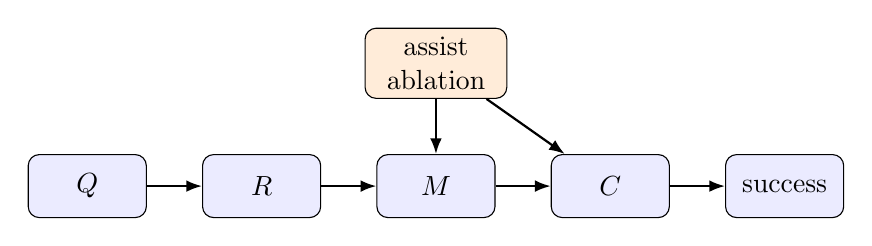
\begin{tikzpicture}[
    node distance=7mm and 7mm,
    box/.style={draw, rounded corners, align=center, minimum height=8mm, minimum width=15mm, fill=blue!8},
    arrow/.style={-{Latex[length=2.0mm]}, thick},
    assist/.style={draw, rounded corners, align=center, minimum height=7mm, minimum width=18mm, fill=orange!15}
  ]
    \node[box] (q) {$Q$};
    \node[box, right=of q] (r) {$R$};
    \node[box, right=of r] (m) {$M$};
    \node[box, right=of m] (c) {$C$};
    \node[box, right=of c] (s) {success};
    \node[assist, above=of m] (a) {assist\\ablation};
    \draw[arrow] (q) -- (r);
    \draw[arrow] (r) -- (m);
    \draw[arrow] (m) -- (c);
    \draw[arrow] (c) -- (s);
    \draw[arrow] (a) -- (m);
    \draw[arrow] (a) -- (c);
  \end{tikzpicture}
  \caption{Stage-structured interpretation of the Q/R/M/C framework. Assist on/off ablations target intermediate mechanisms; in the multi-agent extension the cadence protocol $\mathcal{C}_K$ acts on the R$\to$M and M$\to$C edges.}
  \label{p1:fig:causal}
\end{figure}

\paragraph{Relation to prior work.} Closest are (i) cognitive-map and semantic-map frameworks \citep{tolman1948cognitive,okeefe1978hippocampus,kuipers2000spatial,gupta2017cognitive,savinov2018semi}, (ii) goal-conditioned and successor-representation RL \citep{andrychowicz2017hindsight,ghosh2021learning,dayan1993improving,stachenfeld2017hippocampus,momennejad2017successor}, (iii) multi-agent communication \citep{lowe2017maddpg,foerster2018ctde,sukhbaatar2016commnet,foerster2016learning} and gossip/consensus \citep{boyd2006gossip,xiao2007distributed}, and (iv) LLM-agent memory layers evaluated end-to-end \citep{wang2023voyager,shinn2023reflexion,packer2023memgpt}. Our framework is orthogonal to all four: it \emph{diagnoses} where in the Q/R/M/C chain a given architecture succeeds or fails and lifts the cadence axis from network protocols to a cognitive-architecture parameter (full discussion in Appendix~\ref{p1:app:related-work-extended}).

\subsection{Event semantics, bounded rationality, and an order-theoretic reading}
\label{p1:sec:event-semantics}

The four starred events anchor at concrete logged triggers. We state the triggers once, because every empirical claim in the paper is a claim about them (per-regime formal definitions in Appendix~\ref{p1:app:estimators}), and we give each stage its reading in terms of the resource it bounds.

\begin{description}[leftmargin=10pt,topsep=2pt,itemsep=2pt]
\item[$Q^\star$ (intent issued).] The planner emits a semantic intent $q=(q^{\mathrm{req}},q^{\mathrm{pref}},q^{\mathrm{pen}})$: small sets of required, preferred, and penalty tags. The episode-level event fires on emission, so it is saturated whenever the task is semantic ($\hat P(Q^\star){=}1.00$ in Table~\ref{p1:tab:consistency}); the multi-agent per-tick logger additionally requires a non-empty candidate set (Appendix~\ref{p1:app:multi-agent-defs}), a bookkeeping difference we record rather than hide. Resource bound: attention --- the intent is a few tags, not the full state.
\item[$R^\star$ (memory answers).] Retrieval evaluates $q$ against the memory and returns a candidate set; the event fires when the set contains a candidate satisfying the task predicate (within $\epsilon$ of a true target in the multi-agent logger). The 91\% empty-candidate-set failures of \S\ref{p1:sec:refined-attribution} are $R$-side events: no stored place clears the required-tag threshold. Resource bound: memory --- retrieval can only surface what consolidation has stored.
\item[$M^\star$ (target lock).] The planner materializes one candidate into a concrete actionable cell. Candidacy itself is threshold-gated (a place enters the candidate set only if its score clears the planner's gate, Appendix~\ref{p1:app:schemas}), and the lock commits to a single candidate once per query rather than re-optimizing against the full memory at every tick. The event fires on lock acquisition (within $\epsilon$ of a true target in the multi-agent logger). Resource bound: deliberation.
\item[$C^\star$ (closed-loop completion).] The local controller executes until the locked cell is reached or the episode times out; the event fires on arrival. $C$ is the only stage whose failure modes are extra-semantic: controller competence and, in the multi-agent regime, occupancy $\mathcal{O}_{-i}$. Resource bound: control, and in a collective, shared targets.
\end{description}

\paragraph{Observable-interaction reading.} The four events admit a
uniform reading as semantically distinct acts in the externally
observable interaction, with no reference to internal computational
state: $Q^\star$ is an informational commitment (a query stating what
evidence is needed); $R^\star$ is the memory's answer to that
commitment; $M^\star$ is a public commitment to act on specific
evidence, existing exactly from the moment the lock is written ---
and, in a collective, visible to peers and occupying a target;
$C^\star$ is the environment's confirmation that the commitment was
realized. This grounds Materialization independently of any cognitive
interpretation (the appearance of a public commitment is an objective
log event), and such commitments are the source of the
occupancy contention of \S\ref{p1:sec:multi-agent-results}. The stance
mirrors runtime verification and distributed-system observability,
where specifications constrain externally visible events rather than
internal state \citep{leucker2009runtime}.

\paragraph{Interpretive readings (all deferred).} The stages admit
three readings, none of which is a contribution and all of which now
live in the appendices: the pipeline as a \emph{satisficing, boundedly
rational} agent whose four resource bounds (attention, memory,
deliberation, control) are exactly the four failure loci
(Appendix~\ref{p1:app:hmdp}); an \emph{order-theoretic} account of empty
retrieval --- the $91\%$ regime --- via the query--extent Galois
connection (Appendix~\ref{p1:app:galois}); and an \emph{options/semi-MDP}
account of why optima appear on time-bearing metrics rather than on
the duration-blind chain probability $\Phi$
(Appendix~\ref{p1:app:hmdp}).

\section{Single agent: stage diagnostics localize failure}
\label{p1:sec:single}

\begin{table*}[t]
  \caption{System classes on which the Q/R/M/C contract is evaluated, and where each is reported. The single symbolic agent is the first row; the communicating collective, the learned-communication policies, and the local LLM agents are rows two to four (all instrumented within \S\ref{p1:sec:multi}); the three third-party agent stacks are the last row. ``Stage observability'' records whether the four conditional rates separate: full where an explicit query/lock interface exists, collapsed where a learned channel removes it, and marginal (non-nested event frequencies $f(\cdot)$) where only a tool trace is available.}
  \label{p1:tab:portability}
  \centering
  \small
  \begin{tabular}{p{3.5cm} p{4.6cm} p{3.5cm} c}
    \toprule
    System class & Representative instances & Stage observability & Section \\
    \midrule
    Single symbolic agent & node / concept / state-conditioned stack, four task families & full Q/R/M/C, oracle-testable & \S\ref{p1:sec:single} \\
    Multi-agent symbolic memory & independent / shared bus / central aggregator / peer($K$) & full Q/R/M/C per agent & \S\ref{p1:sec:multi} \\
    Learned communication & CommNet (REINFORCE/PPO), MAPPO & $Q$ saturates, R/M collapse & \S\ref{p1:sec:multi-agent-results} \\
    Local LLM agents & qwen3:4b, llama3.1, Qwen2.5-3B/7B (TextNav) & full; budget$\to$C, capability$\to$R & \S\ref{p1:sec:multi-agent-results} \\
    Third-party agent stacks & OpenAI SDK, LangGraph, AutoGen & marginal frequencies $f(\cdot)$, not nested & \S\ref{p1:sec:external} \\
    \bottomrule
  \end{tabular}
\end{table*}

This section instantiates the first row of
Table~\ref{p1:tab:portability}: a single symbolic agent, the simplest
system class, where the question is whether stage attribution adds
information that end-to-end success does not.

\subsection{System, tasks, and protocol}
\label{p1:sec:single-setup}

\paragraph{Memory stack.}
The system uses a graph substrate with a semantic retrieval interface on top: observations $o_t$ are tokenized into symbolic scene tokens and semantic tags that update a memory of place records, transitions, episodic traces, and concept/relation records. Planner queries return candidates by a weighted log-score over required, preferred, and penalty tags. The retrieval machinery is reused across all tasks and architectures; full memory schema, update rules, and scoring formula are in Appendix~\ref{p1:app:schemas}.

\paragraph{Tasks, baselines, protocol.}
Four single-agent task families are evaluated (water, safe-rest, goal-region on Empty-6x6 / FourRooms~\citep{sutton1999between}, hazard recovery on LavaGapS7), 10 seeds $\times$ 8 episodes each, $\times$ 2 assist modes. Semantic stack (node, concept, state-conditioned variants) is compared against four baselines: random, graph-only, SPTM-like, learned BC. Reported: end-to-end success, steps, four operational stage rates, assist deltas, weakest stage per task and per method. All means are seed-aggregated; 95\% bootstrap CIs use $B{=}5{,}000$ resamples~\citep{efron1979bootstrap}; assist comparisons use paired Wilcoxon signed-rank tests~\citep{wilcoxon1945individual} with Holm-Bonferroni correction~\citep{holm1979simple} (Appendix~\ref{p1:app:assist}). For the two hardest tasks (FourRooms, LavaGapS7), four oracle regimes (\emph{base}, \emph{oracle R/M/C}) are run — each replaces exactly one stage while leaving the rest of the pipeline unchanged. BabyAI portability check in Appendix~\ref{p1:app:babyai}. All single-agent experiments ran on a 10-core ARM CPU, 32\,GB RAM (CPU-only); oracle sweep $<1$\,min wall-clock.

\paragraph{LLM diagnostic block.}
To check that Q/R/M/C is not tied to the symbolic planner implementation, we also run a fixed TextNav substrate with an LLM-driven observe/query/retrieve/decide loop. The TextNav task, prompts, parser contract, and event definitions are held fixed while only the local Ollama model changes; the backend uses model-compatible completion settings when an Ollama chat template otherwise hides short structured answers in a separate thinking field. This block is a controlled step-budget study (Table~\ref{p1:tab:llm-smoke}): sweeping the completion budget drives both LLM agents into a failure that Q/R/M/C localizes to the $C$ stage while $Q/R/M$ stay saturated, exhibiting the framework's diagnostic property on real language agents. Reproducing full ReAct/Reflexion/Voyager/MemGPT-style agents is a separate systems contribution; the comparison to those systems is a coverage comparison in Appendix~\ref{p1:app:sota-coverage}.

\subsection{Stage-estimator validation}
\label{p1:sec:validation}

Before the main benchmark, the factorization is validated. On a
synthetic four-stage process with known probabilities the
nested-estimator product tracks empirical semantic-path completion
across sample sizes. On the real benchmark, the same product matches
semantic-path completion rather than overall success
(Table~\ref{p1:tab:consistency}) --- exactly the contract of
Definition~1.

\begin{table*}[t]
  \caption{Stage-factor consistency audit for the best semantic method in each task family. The product of nested conditional estimators matches semantic-path completion; overall success can be higher because some episodes succeed without traversing the full semantic retrieval path.}
  \label{p1:tab:consistency}
  \centering
  \small
  \begin{tabular}{p{1.7cm}p{2.5cm}c c c c c c c}
    \toprule
    Task & Method & Overall & SP-comp & $\hat P(Q^\star)$ & $\hat P(R^\star|Q^\star)$ & $\hat P(M^\star|R^\star)$ & $\hat P(C^\star|M^\star)$ & Product \\
    \midrule
    Water & \texttt{water-cp} & 0.95 & 0.70 & 1.00 & 0.98 & 0.74 & 0.97 & 0.70 \\
    Rest & \texttt{rest-s2} & 0.93 & 0.73 & 1.00 & 1.00 & 0.80 & 0.91 & 0.73 \\
    Goal region & \texttt{goal-n1} & 0.54 & 0.00 & 1.00 & 0.54 & 0.01 & 0.00 & 0.00 \\
    Hazard recovery & \texttt{hazard-s7} & 0.40 & 0.16 & 1.00 & 0.56 & 0.58 & 0.50 & 0.16 \\
    \bottomrule
  \end{tabular}
\end{table*}

\subsection{Success-only summary and what it hides}
\label{p1:sec:single-results}

Water and rest are strong end-to-end tasks (0.95 and 0.93 success; Figure~\ref{p1:fig:hero}b). Goal-region reaches 0.54 success at the task-family level --- an average that pools a solved environment (Empty-6x6, $1.00$) with a hard one (FourRooms, $0.075$; \S\ref{p1:sec:oracle}), so the family number is bimodal rather than a uniform mid-difficulty --- but the bottleneck sits downstream of candidate selection (\S\ref{p1:sec:oracle}). Hazard recovery is the hardest retrieval-sensitive task at 0.40 success, with retrieval satisfaction as the weakest stage. Under success-only evaluation the two hard families look like the same kind of weakness; the stage view will show they are opposites. Per-task operational rates with 95\% CIs are in Table~\ref{p1:tab:main-results} (Appendix~\ref{p1:app:single-results-table}).

\paragraph{Baseline comparison.}
Table~\ref{p1:tab:baselines} compares the semantic stack against random,
graph-only, SPTM-like, and learned behavior-cloned baselines. The
learned baseline dominates the easiest resource tasks (1.00 on water
and rest) and hazard recovery (0.74), while the semantic stack remains
strongest on the relation-heavy goal-region family (0.54). The
relevant contrast for this paper, however, is not the success column:
the semantic stack is the only method family whose decisions expose
interpretable Q/R/M/C structure. On the BC baseline the stage events
are degenerate for the same structural reason as on the multi-agent
learned baseline analysed in \S\ref{p1:sec:multi-agent-results} --- a
policy without an explicit query/lock interface cannot emit separable
stage events, so the diagnostic decomposition has nothing to attach
to. End-to-end learning and stage diagnostics answer different
questions; this paper is about the second.

\begin{table*}[t]
  \caption{Baseline comparison. The learned behavior-cloned baseline dominates the easiest resource tasks and hazard recovery, while the semantic stack remains strongest on the relation-heavy goal-region family and remains the only family with interpretable Q/R/M/C structure.}
  \label{p1:tab:baselines}
  \centering
  \small
  \begin{tabular}{p{1.9cm}c c c c c}
    \toprule
    Task & Random & Graph-only & SPTM-like & Learned & Best semantic \\
    \midrule
    Water & 0.85 & 0.90 & 0.90 & 1.00 & 0.95 \\
    Rest & 0.85 & 0.90 & 0.90 & 1.00 & 0.93 \\
    Goal region & 0.41 & 0.49 & 0.52 & 0.50 & 0.54 \\
    Hazard recovery & 0.08 & 0.39 & 0.00 & 0.74 & 0.40 \\
    \bottomrule
  \end{tabular}
\end{table*}

\subsection{Oracle-stage interventions localize the bottleneck}
\label{p1:sec:oracle}

On goal-region the semantic variants solve Empty-6x6 ($1.00$ success) but collapse on FourRooms ($0.075$). For hazard recovery (LavaGapS7), base success $0.39$ (bootstrap 95\% CI $[0.35,0.43]$) rises only to $0.43$ under oracle controller, but jumps to $0.59$ under oracle materialization and $0.60$ under oracle retrieval (CI $[0.51,0.69]$; per-seed paired deltas positive in $9/10$ seeds, exact sign test $p{=}0.004$); goal-region rejoin is downstream-limited (oracle R lifts semantic-path completion to $0.08$ without moving end-to-end success). The per-task attribution as a stacked waterfall is in Figure~\ref{p1:fig:oracle-waterfall} (Appendix~\ref{p1:app:single-results-table}). Two tasks identical under success-only evaluation fail at opposite ends of the Q/R/M/C chain.

\subsection{The logs refine the diagnosis: a memory-accumulation limit}
\label{p1:sec:refined-attribution}

Inspecting the framework's own logs sharpens the retrieval attribution. On the 10-seed hazard-recovery run, $349$ retrieval calls were logged: only $32$ ($9.2\%$) returned at least one candidate, and of these $31$ ($96.9\%$ precision) selected a semantically satisfied candidate. The bottleneck is therefore not candidate \emph{ranking} but candidate \emph{generation} --- the symbolic memory does not contain hazard-recovery-tagged nodes at 91\% of decision points. A retrained 2-layer candidate-generation MLP trained on per-state features (test accuracy $0.59$ vs majority-class $0.81$; Appendix~\ref{p1:app:learned-baselines}) confirms that instantaneous state features cannot substitute for the missing structure. The framework's ``retrieval-limited'' attribution thus refines to a \emph{memory-accumulation} limit: candidate generation cannot be solved from state features alone, and the binding constraint is how trajectory evidence is consolidated into persistent symbolic structure. This attribution is not an artefact of the required-tag threshold $\theta$: sweeping $\theta$ across the full range leaves the empty-candidate-set rate invariant (Appendix~\ref{p1:app:theta-robustness}), because the empties are absence of any stored candidate, not sub-threshold filtering. Nor is it an artefact of the weighting: the empty rate is $0.908$ pooled over calls, $0.909$ seed-weighted, and $0.891$ episode-weighted (mean over the 80 episodes of each episode's own empty share), so long failing episodes contributing more decision points do not inflate the figure. Accumulation itself is not one of the four stages: the protocol localized the failure to the R link, and this within-link forensics named the cause --- we read Q/R/M/C as coarse localisation with a designated drill-down, not as a complete causal ontology of memory failure. This sets up the multi-agent section: when consolidation becomes a shared process across $N$ agents, it acquires a measurable \emph{rate}.

\section{Multi-agent: memory as a shared resource}
\label{p1:sec:multi}

This section instantiates rows two to four of
Table~\ref{p1:tab:portability}: the same logged events, unchanged,
instrument a communicating collective --- and, within the same
section, learned policies and LLM agents --- where the additional
failure axis is contention for the targets that memory designates.

\subsection{Four memory architectures and the cadence axis}
\label{p1:sec:archs}

Four communication architectures are instantiated; they share the
single-agent retrieval substrate but differ in how memory is
distributed across agents (Figure~\ref{p1:fig:architectures}).

\begin{figure}[t]
  \centering
  
\includegraphics[width=\linewidth]{figures/fig_architectures.pdf}
  \caption{Four multi-agent memory architectures. \textbf{(a)} Independent: per-agent private memory, no exchange. \textbf{(b)} Shared bus: one global memory, every agent reads/writes each tick. \textbf{(c)} Central aggregator: per-agent memories plus a hub that merges them into a consensus report. \textbf{(d)} Peer-to-peer broadcast: per-agent memories with pairwise snapshot exchange every $K$ ticks (the cadence axis of Empirical Claim~1).}
  \label{p1:fig:architectures}
\end{figure}

\begin{description}[leftmargin=10pt,topsep=2pt,itemsep=2pt]
\item[Independent.] Each agent maintains a private event store and concept graph. No inter-agent communication mechanism exists. Lower-bound baseline.
\item[Shared bus.] All agents publish observations to a single \emph{collective memory} event bus. One shared concept graph is rebuilt from the union of events. Maximally centralized.
\item[Central aggregator (ConsensusLayer).] Each agent has its own private concept graph; a central layer pulls snapshots and computes a trust-weighted merge, producing a single \emph{consensus report} consumed by all agents.
\item[Peer-to-peer broadcast (cadence $K$).] Each agent has its own concept graph and its own merged view. Every $K$ ticks each agent broadcasts a snapshot to a passive bus; each agent independently merges its own snapshot with the latest snapshot received from each peer. Different agents may hold different merged views; there is no central report.
\end{description}

The first three correspond to the three regimes in the multi-agent
communication literature: no exchange, CTDE-style aggregation, and
decentralized peer communication. The fourth is the architecture for
which Definition~2 and Empirical Claim~1 are directly
applicable, since the cadence $K$ is a tunable parameter rather than a
fixed protocol. Mechanically, $K$ is the rate at which private
memories consolidate into a collective view, which is why it is the
structural axis of this section.

\subsection{Multi-agent factorization}
\label{p1:sec:multi-theory}

Extend the factorization to a population of $N$ agents that share
information through a communication protocol $\mathcal{C}_K$
parameterized by broadcast cadence $K$. Each agent $i$ has its own
memory state $\mathcal{M}_i$ and issues its own query $q_i$. Let
$\mathcal{M}_i^{(K)}$ denote the projection of agent $i$'s memory at
the moment it queries, after absorbing every peer message received
under cadence $K$. Two coupling channels are separated: (i) memory
coupling $\mathcal{M}_{-i}^{(K)}$, the latest peer memory snapshots
accessible to agent $i$; (ii) occupancy coupling $\mathcal{O}_{-i}$,
the set of targets that other agents have already claimed by the time
$i$ acts.

\paragraph{Definition 2 (multi-agent stage estimability).}
For each agent $i$,
\[
P(C^\star_i \mid q_i, \mathcal{M}_i, \mathcal{C}_K)
=
P(Q^\star_i \mid q_i, \mathcal{M}_i)\;
P(R^\star_i \mid Q^\star_i, q_i, \mathcal{M}_i, \mathcal{M}_{-i}^{(K)})
\]
\[
\quad \cdot\;
P(M^\star_i \mid R^\star_i, q_i, \mathcal{M}_i, \mathcal{M}_{-i}^{(K)})\;
P(C^\star_i \mid M^\star_i, q_i, \mathcal{O}_{-i}).
\]
Under a multi-agent stage-Markov assumption
(Appendix~\ref{p1:app:estimators}), the four factors are estimable from
per-agent trajectory logs and the empirical-frequency estimators are
consistent.

\paragraph{When Definition~2 may fail.}
The single-agent stage-Markov property absorbs trajectory history into
$(q, \mathcal{M})$. In the multi-agent setting, the analogous
absorption requires that dependence on past peer decisions enters only
through $\mathcal{M}_{-i}^{(K)}$ at the M stage and through
$\mathcal{O}_{-i}$ at the C stage. This step is non-trivial:
$\mathcal{O}_{-i}$ summarises target occupancy at decision time but
loses information about \emph{how} peers arrived there. The
factorization is therefore a projection onto observable per-agent
traces under that summary. Two specific failure modes arise: (i)
inter-agent communication side-channels not logged through
$\mathcal{C}_K$; (ii) coordinated peer policies whose decision at the
C stage depends on hidden peer state not summarised by
$\mathcal{O}_{-i}$.

\subsection{Bottleneck shift}
\label{p1:sec:shift}

\paragraph{Empirical Claim~1 (bottleneck shift M$\leftrightarrow$C, slope-level).}
Assume scarcity ($N > T$ targets, see \S\ref{p1:sec:notation}) and a
peer-broadcast architecture with cadence $K \in \mathbb{N}$. Two
stylized assumptions are posited:
\textbf{(F)} memory freshness $\nu(\mathcal{M}_{-i}^{(K)})$ is
non-decreasing pointwise as $K$ decreases, and the probability that
agent $i$'s planner locks onto a reachable target is non-decreasing in
$\nu$;
\textbf{(O)} the probability that an arbitrary committed target is
already in $\mathcal{O}_{-i}$ is non-increasing as $K$ increases.
Write $P(M^\star|R^\star;K)$ and $P(C^\star|M^\star;K)$ for the
population-level conditional probabilities (averaged over agents and
the seed distribution of the benchmark); $\hat{P}(\cdot)$ denotes the
corresponding empirical-frequency estimator computed from logs. Under
(F) and (O),
\[
\frac{\partial\, P(M^\star|R^\star;K)}{\partial K^{-1}} > 0,
\qquad
\frac{\partial\, P(C^\star|M^\star;K)}{\partial K^{-1}} < 0.
\]
Both slope conditions are direct empirical predictions that are
testable on logs through $\hat{P}$.

\paragraph{What this claim is and is not.}
Empirical Claim~1 is a \emph{slope-level statement on conditional rates}: each of the two slopes is testable and is confirmed on the 35{,}640-run sweep (\S\ref{p1:sec:multi-agent-results}) and independently on a 100-run standard-MiniGrid portability sweep (\S\ref{p1:sec:limitations}). We report the slopes as \emph{effect sizes with cluster-robust confidence intervals} (resampled over the 81 independent configuration cells rather than the correlated run count) in Appendix~\ref{p1:app:effect-sizes}. The claim's boundary with respect to the conditional product $\Phi$ is stated once, in the Scope-and-non-claims box (\S1) and in \S\ref{p1:sec:multi-agent-results}. The shift is a signature of scarce-target contention, not of the grid design: under abundance ($T{>}N$) both slopes flatten and the M$\leftrightarrow$C anticorrelation attenuates (Appendix~\ref{p1:app:cadence-robustness}), i.e.\ the prediction breaks exactly where the contention mechanism is removed.

\paragraph{Chronology.}
Empirical Claim~1 is post-hoc. It was formulated \emph{after} an initial 12{,}960-run sweep conducted under four stage-agnostic hypotheses (Appendix~\ref{p1:app:diagnostics}); the two slope conditions were then confirmed on the full 35{,}640-run sweep, on the $N\!=\!12$ scale-up (Appendix~\ref{p1:app:babyai}), and on the MiniGrid portability wrapper (\S\ref{p1:sec:limitations}). We state this explicitly: the verified slope signs are predictions on enlarged data, not a pre-registered (externally timestamped)
prediction. A fully formal version is left for future work.

\subsection{Sweep protocol}
\label{p1:sec:multi-agent-protocol}

The four architectures are evaluated on a custom multi-agent grid ($12{\times}10$ cells); each agent must reach a cell tagged \texttt{water\_source}, choosing actions via a shared memory-driven planner so only the memory layer differs. The sweep crosses $N{\in}\{3,5,8\}$, $T{\le}N$, three layouts (symmetric/asymmetric/random), three hazard densities, four architectures, eight peer cadences $K{\in}\{1,2,4,8,16,32,48,64\}$, 40 seeds --- 35{,}640 runs in $\approx 22$ min on 8 cores. Per-agent per-tick Q/R/M/C indicators are logged (Appendix~\ref{p1:app:estimators}); episode-level starred events are the disjunction over ticks. A separate oracle-intervention block on scarcity cases $(N,T){\in}\{(3,2),(5,3),(8,5)\}$ at five cadences evaluates oracle R (memory returns ground-truth water positions), oracle M (planner locks onto nearest real water), and oracle C (completion of a real materialized lock is guaranteed; Appendix~\ref{p1:app:oracle-c-def}).

\subsection{Results: stage decomposition and bottleneck shift}
\label{p1:sec:multi-agent-results}

The 35{,}640-run sweep is reported through four observations,
structured to mirror Empirical Claim~1: (i) the conditional
decomposition isolates the M and C stages as the differentiating
links; (ii) the bottleneck shift appears directly as a negative
within-cadence correlation between $P(M^\star|R^\star)$ and
$P(C^\star|M^\star)$, peaking at $K\!=\!4$ and decaying to noise at
$K\!=\!64$; (iii) on mean time-to-success, the resulting trade-off
produces an interior optimum at $K\!=\!8$ --- robust in location but shallow in margin, with the advantage over the adjacent fast cadences not resolved at this sample size (Appendix~\ref{p1:app:effect-sizes}); (iv) on the
conditional product $\Phi$, the same trade-off produces a monotone
trend rather than an interior peak --- a summary statistic on which we make no formal claim. A learned-communication baseline and a multi-agent
oracle-intervention loop close the subsection.

\subsubsection{Conditional decomposition reveals where each architecture fails.}
Figure~\ref{p1:fig:conditional-rates} shows per-architecture conditional Q/R/M/C rates; full numerics with bootstrap CIs are in Appendix~\ref{p1:app:phi-detail}, Table~\ref{p1:tab:multi-agent-cond}. Retrieval conditional $P(R^\star|Q^\star)$ is saturated; the differentiating signal lives at M and C. Shared-bus, central-aggregator, and fast-broadcast peer ($K\le4$) have high $P(M^\star|R^\star)$ but low $P(C^\star|M^\star)$; independent and slow-broadcast peer ($K\ge16$) show the reverse --- the M$\leftrightarrow$C trade-off predicted by Empirical Claim~1.

\begin{figure}[t]
  \centering
  
\includegraphics[width=\linewidth]{figures/fig_conditional_rates.pdf}
  \caption{Per-architecture conditional rates (top) and mean time-to-success among successes (bottom) from the 35{,}640-run sweep. Error bars and band: 95\% cluster-bootstrap CIs over the 81 design cells; points are cell-weighted means ($7.63$ at $K{=}8$ vs.\ $8.04$ independent; the run-pooled values of Table~\ref{p1:tab:multi-agent-cond} are $7.47$/$8.02$). Shared bus, central aggregator, and fast peer broadcast ($K \le 4$) live in the M-saturation / C-collapse regime; independent and slow peer ($K \ge 16$) live in the M-deficit / C-saturation regime. The interior minimum at $K{=}8$ is robust in location but shallow in margin (Appendix~\ref{p1:app:effect-sizes}); the censoring-aware contrast is in the text.}
  \label{p1:fig:conditional-rates}
\end{figure}


\subsubsection{Bottleneck shift and interior efficiency optimum.}
Across all peer runs, Spearman of $P(M^\star|R^\star)$ vs $K$ is $-0.53$ (95\% cluster-robust CI $[-0.59,-0.47]$) and of $P(C^\star|M^\star)$ vs $K$ is $+0.43$ (CI $[+0.37,+0.50]$); both are moderate effect sizes whose CIs exclude zero under resampling of the 81 configuration cells (Appendix~\ref{p1:app:effect-sizes}), matching the slope conditions of Empirical Claim~1. We report these rather than $p$-values, which are uninformative at this correlated sample size. Both slope signs are also robust to the two free thresholds of the logger --- candidacy $\theta$ and lock tolerance $\epsilon$ (Appendix~\ref{p1:app:theta-robustness}). The stronger empirical signature is at the per-configuration level: Pearson of $P(M^\star|R^\star)$ vs $P(C^\star|M^\star)$ \emph{within} a fixed $K$ is $-0.43, -0.54, -0.61, -0.19, -0.05, -0.04, -0.02, -0.02$ at $K{=}1,2,4,8,16,32,48,64$, peaking at $K{=}4$ and decaying to noise by $K{=}64$ (Figure~\ref{p1:fig:jensen-scatter}, Appendix~\ref{p1:app:phi-detail}). Configurations where M is high systematically have low C: the bottleneck migrates between the two stages within the same $(N,T,\text{layout},\text{hazard},\text{seed})$ cell as $K$ varies. On the efficiency metric, mean $t_{\mathrm{succ}}$ has a U-shape with interior minimum at $K{=}8$ (7.47 ticks vs 8.02 for the independent baseline); the minimum's location is robust but shallow --- its margin over the adjacent fast cadences ($K{=}1,4$) is not resolved under cell-level resampling (paired-bootstrap CIs in Appendices~\ref{p1:app:phi-detail} and \ref{p1:app:effect-sizes}). Both statements condition on success. Under a censoring-aware expected time that charges failed runs the full step limit, the fast flank reverses and the independent baseline is marginally best (cell-paired $\Delta(K{=}8-\text{independent}) = +0.32$, CI $[+0.05,+0.63]$; Appendix~\ref{p1:app:effect-sizes}): at fast cadence the completion decline reduces the success rate by more than the materialization gain increases it, so the interior optimum is a statement about conditional speed, not unconditional efficiency --- and closing the unconditional gap is what the reservation protocol of open problem~(3) achieves (Appendix~\ref{p1:app:open-problems}). Scaling to $N{=}12$ \emph{sharpens} the signature: the peak Pearson rises to $-0.70$ and
migrates outward to $K\!=\!8$, consistent with stronger occupancy
coupling at higher $N$ delaying the cost-regime transition
(Appendix~\ref{p1:app:babyai}, Figure~\ref{p1:fig:scale-n12}).

\paragraph{Provenance stratification: the mechanism behind the shift.}
Annotating each $M^\star$ lock with the \emph{provenance} of the
evidence behind it makes the bottleneck shift mechanistic rather than
correlational. Let $\varphi$ be the foreign share of the evidence mass
supporting the locked candidate, computed from the same trust/support
weights the merge itself used and frozen at lock time, and call a lock
a \emph{warp} ($W^\star$) when $\varphi \ge 0.8$: the agent is
committing to a target it knows essentially only from peers. On a
dedicated peer sweep over the scarcity cells (random layouts, 20
seeds, $K\in\{1,2,4,8,16\}$) the warp share $P(W^\star|M^\star)$
falls from $0.55$ at $K{=}1$ to $0.11$ at $K{=}8$ while the
own-evidence stratum completes at a flat $0.26$--$0.34$ and the warp
stratum completes below $0.05$ throughout: \emph{the C-collapse of
fast sharing is concentrated in the warp stratum}. What cadence
controls, mechanically, is how much of the collective's
materialization runs on foreign evidence --- and that is
the stratum whose completions are lost to occupancy contention. The stratification is not
an artefact of the $0.8$ cutoff: recomputed from the raw per-lock
$\varphi$ values ($23{,}237$ locks) at thresholds
$\varphi{\in}\{0.5,0.6,0.7,0.8,0.9,0.95\}$, the foreign stratum
completes at ${\le}0.03$ while the own stratum stays at
$0.26$--$0.50$, at every threshold and cadence. The two coupling
channels also separate interventionally with arms already in the
design: the independent arm removes peer evidence while leaving
target contention in place, and the reservation protocol of open
problem~(3) (Appendix~\ref{p1:app:open-problems}) keeps peer evidence
while managing contention --- under it, unconditional success at fast
cadence exceeds the $K{=}8$ baseline ($0.614$--$0.620$ vs.\
$0.583$; paired improvement over the same cells without the mechanism
$\Delta=+0.037$, cluster-bootstrap 95\% CI $[+0.018,+0.058]$ over 18
matched design cells), identifying occupancy contention rather than
evidence quality as the cost channel of fast sharing. The same stratification
reproduces on the continuous VMAS bridge ($0.72\to0.00$ over
$K{=}1/4/16$) and on an LLM text substrate ($0.42\to0.08$ over
$K{=}2/8$), with the curves nearly coinciding across substrates. A
full provenance-conditioned analysis (counterfactual attribution by
masked replay, a closed-form staleness horizon with a pre-specified
$6/6$-exact hold-out, and a decentralized repair protocol) appears in
a companion manuscript; here the stratification serves as the
mechanistic reading of Empirical Claim~1.

\paragraph{What we do not claim about $\Phi$.} The conditional product $\Phi = P(M^\star|R^\star)\!\cdot\!P(C^\star|M^\star)$ does \emph{not} have an interior peak in the tested range (mean-of-products estimator increases monotonically from $0.569$ at $K{=}4$ to $0.603$ at $K{=}64$, converging to the independent-agent boundary $0.605$). The slope-level statement of Empirical Claim~1 is on the conditional rates themselves, not on $\Phi$; we make no formal claim about the shape of $\Phi(K)$. Jensen-gap detail and POM--MOP comparison in Appendix~\ref{p1:app:phi-detail}.

\paragraph{Learned-communication baseline: stage events are structurally degenerate even at competitive success.}
A CommNet-style policy \citep{sukhbaatar2016commnet} trained with PPO~\citep{schulman2017proximal} on the same scenario ($N{=}3$, $T{=}2$) reaches $0.667$ held-out success ($n{=}100$ seeds) --- matching the symbolic peer architecture at $K{=}8$ ($0.65$). Despite this, the Q/R/M/C profile remains structurally degenerate: $Q^\star{=}1.00$ saturated by construction; $R^\star{=}0.997$, $M^\star{=}0.997$ collapsed together ($P(M^\star|R^\star){=}1.00$). This is the verified structural claim: a real-valued comm vector is never informatively empty (Q saturates) and lacks an explicit target-lock interface (R/M merge), regardless of training budget. The multi-agent counterpart of the single-agent learned-BC analysis (\S\ref{p1:sec:single-results}). Full architecture, PPO hyperparameters, and side-by-side REINFORCE vs PPO comparison in Appendix~\ref{p1:app:learned-baselines}.

\paragraph{LLM model sweep: the logger localizes a real failure in language agents.}
Table~\ref{p1:tab:llm-smoke} runs the same Q/R/M/C event contract on four LLM agents over two independent backends: qwen3:4b and llama3.1 via local Ollama ($8$ episodes/cell), and Qwen2.5-3B/7B-Instruct via HuggingFace transformers on SLURM GPU nodes ($25$ episodes/cell). The decomposition separates \emph{two different failure modes on two different stages}. \textbf{Budget $\to$ C:} below the task's step requirement, three models (qwen3:4b, llama3.1, Qwen2.5-7B) show the identical signature $Q^\star{=}R^\star{=}M^\star{=}1.00$, $C^\star{=}0.00$ --- a completion-limited failure that replicates across backends, model families, and hardware. \textbf{Capability $\to$ R:} Qwen2.5-3B fails at \emph{every} budget with $Q^\star{=}1.00$ but $R^\star{=}0.00$: it declares the target, emits well-formed actions (verified against the response cache, so not a parsing artifact), yet wanders without ever storing the evidence retrieval needs --- an exploration/grounding failure surfacing at the R stage, exactly the ``absence of evidence'' regime of \S\ref{p1:sec:refined-attribution}. An opaque scalar would report both models as $0.00$; the stage view shows they fail for different reasons at different stages. (Instrumentation note: a naive qwen3:4b/Ollama chat-template call initially returned empty \texttt{response} strings because the model spent the short structured-output budget in a separate thinking field; we use raw structured completion for qwen3:4b and a first-line parser, recorded for reproducibility.)

\paragraph{The multi-agent phenomenology reproduces on a live LLM collective.}
Beyond the single-agent budget study, the same event contract
instruments a collective of $N{=}3$ LLM agents (llama3.1) sharing
symbolic place memory by peer broadcast under scarcity ($M{=}2$
takeable targets, four layouts, $K\in\{2,8\}$), with all predictions
specified before the runs. The cadence phenomenology of
\S\ref{p1:sec:multi-agent-results} carries over to the language
substrate: a paired comparison against the no-communication baseline
on identical layouts shows raw sharing \emph{lowering} success from
$2/3$ to $1/3$ per episode --- the occupancy-racing C-collapse, now
produced by agents whose queries, tag extraction, and commitments are
LLM-made --- and target collisions appear in $7/8$ shared-memory
episodes. Attaching the reservation-and-rollback repair protocol (the
constructive answer to open problem~3 of
Appendix~\ref{p1:app:open-problems}) recovers part of the loss
($0.333\to0.417$ at both cadences, rollback latency again
${\approx}K$). Two interface findings transfer to any
LLM-over-symbolic-memory design: LLM query formers free-generate
retrieval tags outside the memory's vocabulary (requiring tolerant
retrieval gates), and small local models are reliable at semantic
commitment but not at coordinate arithmetic or systematic exploration
(requiring layered execution). Full protocol and provenance analysis
in the companion manuscript.

Scope: these are controlled studies on local models; scaling the same contract to full Voyager/MemGPT-style agents on richer tasks with multiple failure modes is developed next (external-framework validation) and in Appendix~\ref{p1:app:sota-coverage}.

\begin{table}[h]
  \caption{LLM TextNav step-budget sweep across four models and two independent backends (local Ollama, $n{=}8$/cell; HuggingFace transformers on a SLURM GPU cluster, $n{=}25$/cell; temperature 0.0; the task needs $\sim$10 low-level steps). Two distinct failure modes are localized to two different stages. \textbf{Budget $\to$ C:} at step limit 6, qwen3:4b, llama3.1 and Qwen2.5-7B all show $Q^\star{=}R^\star{=}M^\star{=}1.00$ with $C^\star{=}0.00$ --- the completion-limited failure replicates across backends, models, and hardware. \textbf{Capability $\to$ R:} Qwen2.5-3B fails at \emph{every} budget ($\{6,8,12,25\}$) with $Q^\star{=}1.00$ but $R^\star{=}0.00$: it declares the target yet never accumulates the evidence to retrieve it (its outputs are well-formed action strings --- verified in the response cache --- so this is an exploration/grounding failure feeding retrieval, not a parsing artifact). Artifacts: \texttt{tmp/llm\_steplimit\_*}, \texttt{tmp/cluster/textnav*}.}
  \label{p1:tab:llm-smoke}
  \centering
  \small
  \begin{tabular}{l l c c c c c c}
    \toprule
    Model & Backend & Step limit & Success & $Q^\star$ & $R^\star$ & $M^\star$ & $C^\star$ \\
    \midrule
    qwen3:4b        & ollama & 6  & 0.00 & 1.00 & 1.00 & 1.00 & \textbf{0.00} \\
    llama3.1        & ollama & 6  & 0.00 & 1.00 & 1.00 & 1.00 & \textbf{0.00} \\
    Qwen2.5-7B      & hf     & 6  & 0.00 & 1.00 & 1.00 & 1.00 & \textbf{0.00} \\
    \midrule
    qwen3:4b        & ollama & 12 & 1.00 & 1.00 & 1.00 & 1.00 & 1.00 \\
    llama3.1        & ollama & 12 & 1.00 & 1.00 & 1.00 & 1.00 & 1.00 \\
    Qwen2.5-7B      & hf     & 12 & 1.00 & 1.00 & 1.00 & 1.00 & 1.00 \\
    \midrule
    Qwen2.5-3B      & hf     & 6--25 & 0.00 & 1.00 & \textbf{0.00} & 0.00 & 0.00 \\
    \bottomrule
  \end{tabular}
\end{table}

\paragraph{Multi-agent oracle interventions close the diagnose$\to$intervene$\to$verify loop.}
On the scarcity cases, mean $t_{\mathrm{succ}}$ at small/intermediate cadence ($K{\in}\{1,2,4\}$) drops from $\sim10$--$11$ in baseline to $\sim7.2$ under either oracle R or oracle M, and further to $\sim6.1$ under oracle C, which additionally removes post-lock travel; at slow cadence ($K{=}16$) the baseline is already within $\sim1.2$ of the R/M oracle floor (Table~\ref{p1:tab:multi-agent-oracle} in Appendix~\ref{p1:app:multi-oracle}). Crucially, oracle C gives the largest time reduction but the smallest success-rate gain (Appendix~\ref{p1:app:oracle-c-def}): in scarcity, completion costs time while retrieval and materialization decide success. The cadence-induced excess time at small/intermediate $K$ is attributable to the M$\leftrightarrow$C transition; at large $K$ the bottleneck has moved into solo exploration.

The multi-agent block thus delivers its half of the argument. The
cadence $K$ is, mechanically, the rate at which private memories
consolidate into a collective view; the data show that this rate has a
non-trivial interior optimum ($K\!=\!8$ on $t_{\mathrm{succ}}$), that
its cost channel is occupancy coupling, and that both effects are
visible stage-by-stage on the same Q/R/M/C chain used for single
agents. Consolidation is not only the single-agent limit; in a
collective it is a tunable, measurable design axis.

\section{The contract on third-party agent stacks}
\label{p1:sec:external}

This section instantiates the last row of
Table~\ref{p1:tab:portability}. We further evaluate the protocol on
systems built by others. The contract has two layers: an \emph{invariant core} --- four event
roles (a memory query is issued; returned evidence satisfies the
task; the agent commits to a target; the task completes) --- and a
\emph{system-specific adapter} that maps logged actions to those
roles. We instrument three third-party agent stacks --- a
function-calling loop on the OpenAI SDK, LangGraph's prebuilt ReAct
agent, and AutoGen's AssistantAgent/UserProxy pair, all driving the
same local model (llama3.1, temperature $0$) --- with one tool-trace
adapter shared by all three: an episodic household memory is exposed
through \method{recall}/\method{goto}/\method{take} tools, and
$Q^\star$ fires on querying memory, $R^\star$ on \emph{attribution}
(a returned record names the item at its true place), $M^\star$ on a
commitment (a \method{goto} to the true place; first-commitment
accuracy $M_1$ is logged as an auxiliary lock-quality diagnostic),
and $C^\star$ on task completion within a tool budget. A tool trace
exposes no lock chain, so these are \emph{marginal event frequencies}
$f(\cdot)$ in the sense of Appendix~\ref{p1:app:estimators}: an agent
can commit to the true place without a supporting retrieval, the
events are not nested, and no factorisation is claimed --- the four
frequencies serve as separate diagnostics and are never substituted
into the chain-rule product. What varies across system
classes is the adapter, not the event roles. Three variants engineer
one failure each --- a consolidation gap (the location fact was never
written to memory), a stale-distractor ambiguity, a tool budget below
the task's requirement --- plus a clean control; all predictions were
specified before the runs, and the two revisions of the adapter (an
attribution leak; an over-tightened $M^\star$) are recorded in the
registration file.

\begin{table}[h]
\caption{Marginal Q/R/M/C event frequencies on three third-party
agent frameworks (llama3.1, 20 episodes per cell, identical
episodes/tools/budgets). Each entry is the fraction of episodes in
which the event occurred: $Q^\star$ --- the agent queried memory at
least once; $R^\star$ --- a returned record named the item at its
true place; $M^\star$ --- the agent committed (\method{goto}) to the
true place, with or without retrieval support; $C^\star$ ---
\method{take} succeeded within the tool budget; $M_1$: first
\method{goto} targets the true place; stale$_1$: first \method{goto}
targets the stale distractor. The events are not nested and no
product is claimed (Appendix~\ref{p1:app:estimators}): under the
consolidation gap, budgeted blind search over the four places
sometimes commits to and reaches the true place, hence
$M^\star, C^\star > 0$ at $R^\star{=}0$. Structural failures localize
identically everywhere: the consolidation gap is $R^\star{=}0.00$ and
the budget failure is $C^\star{=}0.00$ at $Q^\star{=}R^\star{=}1$,
for all three stacks. On the \emph{clean} control the frameworks
spread from $0.50$ to $0.75$ end-to-end --- and the decomposition
attributes the spread (see text).}
\label{p1:tab:external}
\centering
\small
\begin{tabular}{llcccccc}
\toprule
Framework & Variant & $f(Q^\star)$ & $f(R^\star)$ & $f(M^\star)$ & $f(C^\star)$ & $f(M_1)$ & $f(\text{stale}_1)$ \\
\midrule
OpenAI SDK & control     & 1.00 & 1.00 & 0.85 & 0.75 & 0.25 & --- \\
           & consolidation gap & 1.00 & \textbf{0.00} & 0.50 & 0.40 & 0.25 & --- \\
           & stale ambiguity   & 1.00 & 1.00 & 0.90 & 0.30 & 0.25 & 0.20 \\
           & tight budget      & 1.00 & 1.00 & 0.25 & \textbf{0.00} & 0.25 & --- \\
\midrule
LangGraph  & control     & 1.00 & 1.00 & 0.70 & 0.50 & 0.50 & --- \\
           & consolidation gap & 1.00 & \textbf{0.00} & 0.20 & 0.15 & 0.10 & --- \\
           & stale ambiguity   & 1.00 & 1.00 & 0.65 & 0.60 & 0.50 & 0.35 \\
           & tight budget      & 1.00 & 1.00 & 0.10 & \textbf{0.00} & 0.10 & --- \\
\midrule
AutoGen    & control     & 1.00 & 1.00 & 0.85 & 0.55 & 0.45 & --- \\
           & consolidation gap & 1.00 & \textbf{0.00} & 0.30 & 0.20 & 0.15 & --- \\
           & stale ambiguity   & 1.00 & 1.00 & 0.50 & 0.45 & 0.35 & 0.40 \\
           & tight budget      & 1.00 & 1.00 & 0.15 & \textbf{0.00} & 0.15 & --- \\
\bottomrule
\end{tabular}
\end{table}

\begin{figure}[t]
\centering

\includegraphics[width=\linewidth]{figures/fig_external_stages}
\caption{Stage profiles of three third-party agent stacks on the four
engineered variants (llama3.1, $n{=}20$ per cell). Query and retrieval
saturate identically everywhere; the two structural failures produce
exact zero columns on every stack ($R^\star{=}0$ under the
consolidation gap, $C^\star{=}0$ under the tight budget); the
behavioral spread between frameworks lives entirely in the M and C
stages.}
\label{p1:fig:external-stages}
\end{figure}

Three findings (Table~\ref{p1:tab:external},
Figure~\ref{p1:fig:external-stages}). \textbf{(1) Structural
localizations are exact and framework-independent.} When the memory
lacks the fact, $R^\star{=}0.00$ on every stack; when the budget
cannot fit completion, $C^\star{=}0.00$ at $Q^\star{=}R^\star{=}1$ on
every stack ($20/20$ episodes each). The contract needs no
per-framework adaptation. \textbf{(2) The clean control separates the
frameworks, and the decomposition says how.} End-to-end success on the
SAME clean episodes ranges $0.50$ (LangGraph) to $0.75$ (OpenAI SDK).
The stage profiles attribute the spread to a failure mode common to
all three stacks combined with framework-specific recovery:
first-commitment accuracy is low everywhere ($M_1{=}0.25$--$0.50$ --- the agent's
first \method{goto} frequently ignores its own just-retrieved
evidence), episode-level materialization recovers to $0.70$--$0.85$
through re-query loops, and the frameworks then differ in how much of
that recovery survives to completion ($C^\star/M^\star$ from $0.88$
for the OpenAI SDK loop down to $0.65$ for AutoGen). \textbf{(3) The
stale distractor pulls, measurably and unevenly.} The outdated record
captures the first commitment in $0.20$--$0.40$ of ambiguous episodes
(most strongly for AutoGen), and its completion cost is
framework-specific: the OpenAI SDK loop pays hardest
($C^\star:0.75\to0.30$) while LangGraph and AutoGen absorb the detour
($0.50\to0.60$; $0.55\to0.45$) --- the LLM-memory analogue of the
staleness gating that the collective experiments showed to be
decisive. Failed pre-specifications and subsequent revisions: the behavioral predictions
that assumed a clean control (all stages $\ge 0.75$; a uniform
ambiguity-induced completion drop) broke \emph{because the frameworks
themselves fail a clean memory task 25--50\% of the time and pay for
ambiguity in different places} --- which is finding (2)--(3), not
noise; all revisions are recorded as failed pre-specifications with
mechanisms.

\paragraph{Model robustness: the structure transfers, the behavior is
legible.} A prediction specified before the runs --- the structural
localizations transfer to a second model on all frameworks, while
behavioral rates are model-dependent and only reported --- was
confirmed exactly by repeating all 240 episodes with qwen3:4b
(Table~\ref{p1:tab:external-qwen}): $R^\star{=}0.00$ under the
consolidation gap and $C^\star{=}0.00$ under the tight budget, $20/20$
on every stack, for both models. The behavioral contrast is a
diagnostic result: qwen3:4b completes every clean episode
($C^\star{=}1.00$ across stacks, vs.\ $0.50$--$0.75$ for llama3.1)
because its \emph{first-commitment accuracy} is high
($M_1{=}0.90$--$0.95$ vs.\ $0.25$--$0.50$) and its susceptibility to
the stale distractor low ($0.05$--$0.30$) --- except under AutoGen,
where qwen's $M_1$ collapses to $0.40$ while remaining $\ge 0.90$ on
the other stacks. The stage decomposition thus separates three
influences a leaderboard conflates: the task's structural limits
(model- and framework-independent), the model's commitment quality,
and the framework's prompt/loop shaping that can degrade it.

\paragraph{Comparison with diagnostic baselines.} On the blinded
benchmark below we additionally evaluate four alternative diagnostics
of the same logs, each receiving the identical anonymized cell
aggregates and calibration control, with decision rules fixed before
scoring and thresholds matched to the Q/R/M/C rule
(\texttt{experiments/qrmc\_external/diagnostic\_baselines.py};
specification in \texttt{tmp/qrmc\_external/baselines\_spec.json}).
Over 63 scored cells (10 faults + held-out control, three stacks, two
models): a success-only reading names no stage ($0.095$); an
AgentBoard-style progress scale (first milestone drop) reaches
$0.730$ (macro-F1 $0.698$); a RAGChecker-style two-stage
retrieval/execution split reaches $0.651$ exact / $0.873$ side-level
(macro-F1 $0.450$), its deficit concentrated where commitment must be
separated from execution; a process-conformance first-deviation rule
using the order-sensitive $M_1$ reaches $0.778$ (macro-F1 $0.755$),
its entire deficit being the budget-exhaustion branch of the
conditional reading; a multinomial logistic regression on the same
aggregates reaches $0.444$ on unseen fault types with a
false-positive rate of $1.00$ on held-out controls (leave-one-model
-out $0.794$, leave-one-framework-out $0.825$) and requires fault
labels that the rule-based methods do not. Q/R/M/C attains $0.873$
(macro-F1 $0.835$; bootstrap CI over fault types $[0.71,0.98]$) and
outperforms all exact-stage alternatives under paired McNemar
tests, with all comparisons significant after Holm correction
(largest adjusted $p=0.031$; discordant cells from $6{:}0$ to
$50{:}1$). Of the $66$ cells, three (the prompt-only fault under
llama3.1) failed the pre-specified manipulation check and are
excluded for every method alike, leaving $63$. A
follow-up repair study (llama3.1, 2{,}640 episodes; pre-specified
menu of stage-level repairs, each diagnostic selecting the repair for
its predicted stage) gives Q/R/M/C the highest completion gain and
lowest regret against the best available arm ($0.293$/$0.061$ vs.\
an oracle-best gain of $0.354$; two-stage $0.280$/$0.074$;
conformance $0.250$/$0.104$; progress $0.219$/$0.135$; random
$0.113$/$0.240$). Paired bootstrap over fault--framework cells
resolves the gain advantage over the progress baseline
($+0.074$ $[+0.007,+0.157]$) but not over the two-stage baseline
($+0.013$ $[-0.009,+0.039]$), which also selects the single best arm
slightly more often ($0.704$ vs.\ $0.630$) because its coarse
diagnoses map to repairs that frequently coincide with the best
available arm; the four-stage advantage is established at exact
localization, while on repair utility the protocol at least matches
the strongest coarse baseline. Two pre-specified expectations failed:
the matched repair for silent corruption recovers only
$0.22$--$0.44$ of the control gap (consolidation without decoy
removal converts a retrieval fault into an ambiguity fault), and the
budget repair on the clean OpenAI SDK control lowered completion by
$0.15$.

\paragraph{Blinded fault-localization meta-evaluation (pre-specified).}
The engineered variants verify localization of failures whose stage
is known by construction; the blinded meta-evaluation treats the protocol
as a \emph{classifier}. We injected ten fault types --- two to three
per stage, structural and behavioral (Table~\ref{p1:tab:meta-eval}) ---
and fixed a first-failing-link decision rule, with all thresholds,
\emph{before} any run (\texttt{tmp/qrmc\_external/registered\_meta.json};
rule and thresholds in
\texttt{experiments/qrmc\_external/run\_meta\_evaluation.py}). The
rule receives only anonymised marginal profiles plus a labelled
control cell for calibration; a held-out control (seeds 20--39)
enters the blind set with ground truth ``none'', measuring the
false-positive rate; a manipulation check excludes faults that do not
bind (the prompt-only fault moved qwen but not llama). Stage-level
accuracy: $26/30$ scored cells for llama3.1 ($8/10$, $8/10$, $10/10$
per stack) and $29/33$ for qwen3:4b ($9/11$, $10/11$, $10/11$); the
five structural faults localize $30/30$ across both models and all
stacks; held-out controls read ``none'' in $5/6$ cells (one false
positive at $n{=}20$); cross-framework label agreement is $7/11$
(llama) and $10/11$ (qwen). The pre-specified model-contrast prediction
was confirmed in its named direction: M-family faults hide behind
llama's weak baseline commitment ($M_1{=}0.25$--$0.50$) and become
visible on qwen's clean baseline --- the unmarked duplicate drops
$M_1$ by $0.90/0.80/0.20$ across stacks --- while its accuracy clause
held on two of three stacks (AutoGen: $10/11$ vs.\ llama's $10/10$,
a one-cell difference). One pre-specified risk materialized
instructively: the \emph{marked} stale distractor changes llama3.1's behavior but
reads ``none'' on qwen3:4b, which takes the staleness marker into
account --- the protocol measures the behavioral effect of a fault,
not its presence, and a fault a model neutralizes is reported as no
failure.

\begin{table}[h]
\caption{Blinded fault localization: injected fault, ground-truth
stage, and correct-localization count over the three stacks, per
model. ``Neutralized'': the fault does not change qwen's behavior
(the staleness marker is heeded), so the blind rule reads ``none''.}
\label{p1:tab:meta-eval}
\centering
\small
\begin{tabular}{llcc}
\toprule
Injected fault & Stage & llama3.1 & qwen3:4b \\
\midrule
recall tool absent        & Q & 3/3 & 3/3 \\
prompt: memory unreliable & Q & non-binding & 3/3 \\
fact never consolidated   & R & 3/3 & 3/3 \\
silent corruption         & R & 3/3 & 3/3 \\
flaky recall ($p{=}0.7$)  & R & 3/3 & 3/3 \\
stale distractor (marked) & M & 1/3 & 0/3 (neutralized) \\
duplicate (unmarked)      & M & 2/3 & 3/3 \\
budget below requirement  & C & 3/3 & 3/3 \\
flaky goto ($p{=}0.5$)    & C & 2/3 & 3/3 \\
take always fails         & C & 3/3 & 3/3 \\
\midrule
held-out control          & none & 3/3 & 2/3 \\
\bottomrule
\end{tabular}
\end{table}

\begin{table}[h]
\caption{Second-model replication (qwen3:4b, 20 episodes per cell,
identical episodes/tools/budgets; thinking disabled request-level for
budget parity, recorded in the pre-run specification). Entries are marginal
event frequencies $f(E)$ as in Table~\ref{p1:tab:external} --- not
chain-rule links. Structural zeros transfer exactly; behavioral
rates differ from llama3.1 (Table~\ref{p1:tab:external}) in the
direction the $M_1$ diagnostic explains.}
\label{p1:tab:external-qwen}
\centering
\small
\begin{tabular}{llcccccc}
\toprule
Framework & Variant & $f(Q^\star)$ & $f(R^\star)$ & $f(M^\star)$ & $f(C^\star)$ & $f(M_1)$ & $f(\text{stale}_1)$ \\
\midrule
OpenAI SDK & control     & 1.00 & 1.00 & 1.00 & 1.00 & 0.95 & --- \\
           & consolidation gap & 1.00 & \textbf{0.00} & 0.45 & 0.45 & 0.20 & --- \\
           & stale ambiguity   & 1.00 & 1.00 & 1.00 & 0.95 & 0.90 & 0.05 \\
           & tight budget      & 1.00 & 1.00 & 0.30 & \textbf{0.00} & 0.30 & --- \\
\midrule
LangGraph  & control     & 1.00 & 1.00 & 1.00 & 1.00 & 0.90 & --- \\
           & consolidation gap & 1.00 & \textbf{0.00} & 0.60 & 0.60 & 0.30 & --- \\
           & stale ambiguity   & 1.00 & 1.00 & 0.95 & 0.95 & 0.75 & 0.20 \\
           & tight budget      & 1.00 & 1.00 & 0.15 & \textbf{0.00} & 0.15 & --- \\
\midrule
AutoGen    & control     & 1.00 & 1.00 & 1.00 & 1.00 & 0.40 & --- \\
           & consolidation gap & 1.00 & \textbf{0.00} & 0.55 & 0.50 & 0.30 & --- \\
           & stale ambiguity   & 1.00 & 1.00 & 1.00 & 0.90 & 0.40 & 0.30 \\
           & tight budget      & 1.00 & 1.00 & 0.15 & \textbf{0.00} & 0.15 & --- \\
\bottomrule
\end{tabular}
\end{table}

Scope: three stacks at $n{=}20$ per cell on two local models;
Letta/CrewAI (Python $\ge$3.10) and API-scale models are the natural
extension.

\section{Limitations and future work}
\label{p1:sec:limitations}

\textbf{Portability across substrates: slope conditions hold on MiniGrid.} The slope conditions of Empirical Claim~1 also hold on a standard-MiniGrid substrate. A FourRooms-based multi-agent wrapper (built from \texttt{minigrid.core.grid.Grid} + Wall/Floor/Lava primitives, identical operational $Q^\star,R^\star,M^\star,C^\star$ definitions; \texttt{experiments/minigrid\_multiagent\_wrapper/}) was used to run a 100-run portability sweep ($K{\in}\{1,4,8,16,64\}$, 20 seeds, $N{=}3$, $T{=}2$): Spearman $P(M^\star|R^\star)$ vs $K$ is $-0.50$ and Spearman $P(C^\star|M^\star)$ vs $K$ is $+0.50$ (moderate rank correlations; this is a small 100-run sweep, so we report the effect sizes and do not lean on significance). The interior $t_{\mathrm{succ}}$ minimum does not separate at this minimal sweep size (5 cadences, 20 seeds, one hazard density); a denser sweep is the natural next step. The two-substrate seam is therefore closed at the slope-level claim.

\textbf{Empirical Claim~1 is slope-level on conditional rates only.} The two slope conditions hold as moderate, cluster-robust effect sizes (Appendix~\ref{p1:app:effect-sizes}); we make no formal claim on the shape of the conditional product $\Phi$ (\S\ref{p1:sec:shift}). A future statement directly in terms of the time-cost surface, or a derivation under a generative model (Poisson-renewal memory, birth-death occupancy), would convert the empirical claim into a theorem.

\textbf{Estimability under hidden state.} With unlogged in-episode query rewrites or peer side-channels, Definitions~1 and~2 are projections onto logged traces, not full identification.

\textbf{Shared coordinate frame.} All multi-agent results assume agents
interpret places in a common coordinate frame: cross-agent place
identity is coordinate proximity, with semantic profiles as a
tie-breaker inside a spatial radius. The place-correspondence problem
--- whether two agents' records denote the same place at all --- is
therefore bracketed here, not solved. A companion manuscript removes
the assumption constructively (fingerprint-based place identity with
consensus frame recovery up to translation and $90^\circ$ rotation)
and shows the Q/R/M/C measurements, including the cadence slopes and
the staleness horizon, unchanged on top of the recovered frames; the
harder variants (continuous $SE(2)$, appearance noise, symbol
alignment) remain open.

\textbf{The evaluator's correspondence oracle.} A deeper form of the
same dependence survives every representational relaxation, and we
state it explicitly. The protocol unifies \emph{observation points},
not internal representations --- but scoring the two middle stages
presupposes an \emph{entity correspondence} between memory content and
world referents: $R^\star$ asks whether a returned candidate denotes
the true target, $M^\star$ whether the lock does. In every study here
that oracle is supplied by an instrumented environment (ground-truth
cells on the grids; the task's true location in the tool-trace
contract). The dependence is graded, which is what makes the protocol
degrade gracefully rather than break: $Q^\star$ requires no
correspondence at all (did the agent query its memory), $C^\star$ is
behaviorally observable (did the task complete), while $R^\star$ and
$M^\star$ --- the diagnostic payload --- are undefined
without it. The severity of the requirement depends on the population
under evaluation: interchangeable agents (a shared perception
interface, possibly different weights) situated in a single
environment inherit the correspondence from the shared substrate ---
the setting of every study in this paper and the common case in
multi-agent evaluation. It becomes a genuinely open problem for
heterogeneous agents in open worlds, where deploying the protocol
requires either an instrumented task or a correspondence mechanism
with its own error model; the companion's meaning-based place identity
is a candidate for grounding the \emph{evaluator's} correspondence,
not only the agents', and we leave that construction open.

\textbf{Learned baselines.} The CommNet PPO baseline reaches $0.667$ success on the scarcity scenario --- competitive with symbolic peer at $K{=}8$ ($0.65$) --- and confirms Q-saturation ($Q^\star{=}1.00$) and R/M collapse ($P(M^\star|R^\star){=}1.00$) at competitive success. The structural prediction now holds verified, not asserted; ablating on architectures with explicit symbolic target-lock channels is left for future work.

\textbf{Scale.} Multi-agent sweep bounded at $N{=}12$ (Appendix~\ref{p1:app:babyai}; signature sharpens, peak Pearson $-0.70$ at $K{=}8$, interior $t_{\mathrm{succ}}$ minimum $4.77$). Denser scaling at $N{\ge}16$ is future work.
\textbf{Continuous substrate.} A VMAS~\citep{bettini2022vmas} validation reproduces \emph{both} slope signs of Empirical Claim~1 across three scarcity cells $\times$ 40 seeds with block-bootstrap CIs excluding zero (Spearman $-0.999$ $[-1.000,-0.975]$ and $+0.995$ $[+0.900,+1.000]$ over $K{\le}16$; Appendix~\ref{p1:app:vmas}), reusing the symbolic memory through a discretisation bridge. The shift is therefore not an artefact of grid cells; what remains open is fully continuous \emph{memory} (the bridge discretises it) and visually rich 3D substrates.

\section{Broader impacts}

The paper proposes diagnostic evaluation for memory-based agents in simulated navigation. Its positive impact is methodological: making memory-based failures more measurable across architectures, and making the cadence axis of distributed multi-agent memory tunable on an empirically grounded criterion. Potential negative impacts are indirect and would arise if similar diagnostics were used to improve agents in safety-critical settings (drone swarms, autonomous vehicles, distributed sensor networks) without adequate safeguards. The current work is benchmark-level infrastructure, not a deployment-ready system.

\section{Conclusion}

We introduced Q/R/M/C as an operational protocol for evaluating
memory-based navigation through four observable stages: query
formation, retrieval satisfaction, target materialization, and
post-retrieval completion. The framework does not replace final task
metrics; rather, it identifies which part of the memory-to-action
pipeline limits performance and whether the relevant stages are
observable in a given architecture.

Across the single-agent experiments, stage-specific interventions
separate retrieval-limited and downstream-limited tasks that appear
similar under success-only evaluation. The detailed retrieval logs
further show that the principal failure is the absence of eligible
memory records rather than poor ranking. In the multi-agent setting,
the same protocol reveals a cadence-dependent shift between
materialization and completion: fast sharing improves access to target
information but increases contention for scarce targets. Experiments
with learned communication policies, local LLM agents, and
third-party agent stacks show that the event contract transfers across
implementations, while also exposing cases in which the architecture
does not provide an explicit stage interface.

The present evidence supports Q/R/M/C as a reproducible diagnostic
layer for systems with observable query and commitment events. It does
not establish a universal decomposition for opaque policies or a
general theorem about the optimal communication cadence. Richer
continuous and visually grounded environments, learned memory
formation, and entity correspondence across heterogeneous agents
remain directions for subsequent parts of the program.

\begin{ack}
This manuscript is prepared in anonymized form for review. The
reported experiments were run from a unified benchmark pipeline that
exports task-family summaries, assist on/off comparisons, method
diagnostics, multi-agent sweep CSVs, and bootstrap analyses from the
same source-of-truth benchmark artifacts.
\end{ack}

{\small

}

\FloatBarrier
\begin{center}\rule{0.55\linewidth}{0.4pt}\\[2pt]\textbf{Appendix material of this part}\end{center}

\section{Formal proofs}
\label{p1:app:proofs}

\subsection{Argument for Definition~1 (single-agent estimability)}

For each episode $i \in \{1,\dots,n\}$ let $Q_i^\star, R_i^\star, M_i^\star, C_i^\star$ denote the nested episode-level indicators. By construction these are measurable functions of the runtime trajectory log and satisfy $C_i^\star \Rightarrow M_i^\star \Rightarrow R_i^\star \Rightarrow Q_i^\star$. The empirical estimators
\[
\hat p_Q = \tfrac{1}{n}\sum_i Q_i^\star,\quad
\hat p_{R|Q} = \tfrac{\sum_i R_i^\star}{\sum_i Q_i^\star},\quad
\hat p_{M|R} = \tfrac{\sum_i M_i^\star}{\sum_i R_i^\star},\quad
\hat p_{C|M} = \tfrac{\sum_i C_i^\star}{\sum_i M_i^\star}
\]
are consistent by the chain rule plus the conditional stage-Markov property, and the empirical product converges to semantic-path completion. \hfill$\square$

\subsection{Argument for Definition~2 (multi-agent estimability)}

Conditioning sets are enlarged by $\mathcal{M}_{-i}^{(K)}$ and $\mathcal{O}_{-i}$. Under the enlarged stage-Markov property, the proof of Definition~1 transfers verbatim and each enlarged conditional is a Bernoulli probability on a measurable event. The qualifications stated in \S\ref{p1:sec:multi-theory} (``When Definition~2 may fail'') describe two specific situations in which the enlarged stage-Markov property is violated. \hfill$\square$

\subsection{Argument for Empirical Claim~1 (slope-level statement)}

Empirical Claim~1 is an empirical claim, not a theorem. The argument below is the qualitative justification that motivates the two slope signs; the data are what verify them. We deliberately do not call this a proof.

\emph{Slope (a), under (F).} As $K$ decreases, $\nu(\mathcal{M}_{-i}^{(K)})$ is non-decreasing pointwise. Conditional on a successful retrieval, the probability of locking onto a reachable target is non-decreasing in $\nu$. Therefore $\partial P(M^\star|R^\star;K) / \partial K^{-1} > 0$.

\emph{Slope (b), under (O).} As $K$ decreases, peers receive updated memory simultaneously and converge on the same closest target; the marginal occupancy $\Pr[\text{target}\in\mathcal{O}_{-i}]$ rises. Therefore $\partial P(C^\star|M^\star;K) / \partial K^{-1} < 0$.

\emph{Note on the conditional product $\Phi$.} Empirical Claim~1 makes no statement about the shape of $\Phi(K) = P(M^\star|R^\star;K)\!\cdot\!P(C^\star|M^\star;K)$. Under (F) and (O) the slope of $\Phi$ in $K^{-1}$ is the sum of two opposing terms, and whether it changes sign depends on quantitative magnitudes that are not pinned down by (F) and (O) alone. In our data $\Phi$ is monotone in $K$ over $\{4,8,16,32,48,64\}$ and converges to the independent-agent boundary $\Phi_\infty = 0.605$. The practically relevant efficiency surface --- mean time-to-success --- does have an interior minimum at $K=8$; see \S\ref{p1:sec:multi-agent-results}. \hfill$\square$

\subsection{The query--retrieval Galois connection: statement, argument, scope}
\label{p1:app:galois}

\paragraph{Fact (standard).}
Let $G$ and $\Sigma$ be sets and $I \subseteq G \times \Sigma$ a relation. For $B \subseteq \Sigma$ define $\mathrm{ext}(B) = \{p \in G : \forall \tau \in B,\ (p,\tau) \in I\}$, and for $A \subseteq G$ define $\mathrm{int}(A) = \{\tau \in \Sigma : \forall p \in A,\ (p,\tau) \in I\}$. Then for all $A \subseteq G$, $B \subseteq \Sigma$:
\[
A \subseteq \mathrm{ext}(B) \iff B \subseteq \mathrm{int}(A);
\]
both maps are antitone, both composites $\mathrm{ext}\circ\mathrm{int}$ and $\mathrm{int}\circ\mathrm{ext}$ are closure operators, and the closed pairs $(A, B)$ with $A = \mathrm{ext}(B)$ and $B = \mathrm{int}(A)$, ordered by extent inclusion, form a complete lattice --- the concept lattice of the context $(G, \Sigma, I)$ \citep{ganter1999fca}.

\paragraph{Argument.}
$A \subseteq \mathrm{ext}(B)$ unfolds to $\forall p \in A\ \forall \tau \in B:\ (p,\tau) \in I$, a condition symmetric in $A$ and $B$, which is exactly $B \subseteq \mathrm{int}(A)$. Antitonicity and the closure properties follow by the standard one-line arguments \citep[Ch.~1]{ganter1999fca}. Viewing the power sets as thin categories (one with reversed order), the displayed equivalence says precisely that $\mathrm{int}$ and $\mathrm{ext}$ form an adjoint pair; a Galois connection is an adjunction between posets \citep[Ch.~IV]{maclane1998categories}. \hfill$\square$

\paragraph{Instantiation and scope.}
In our memory, take $G$ to be the place records, $\Sigma$ the tag alphabet, and $I_\theta = \{(p,\tau) : \text{the per-place tag table assigns } \tau \text{ to } p \text{ with confidence} \ge \theta\}$ (Appendix~\ref{p1:app:schemas}); the intent of a query is $B = q^{\mathrm{req}}$ and R-availability is $\mathrm{ext}(B) \ne \emptyset$. Three deliberate scope restrictions. (i) \emph{Graded scores.} The deployed retrieval score is graded (the weighted log-score over required, preferred, and penalty tags of Appendix~\ref{p1:app:schemas}), so the crisp connection above formalizes the thresholded required-tag skeleton of candidacy; the graded analogue is the theory of fuzzy Galois connections \citep{belohlavek1999fuzzy} and we do not use it here. (ii) \emph{Non-monotone updates.} Dirichlet--multinomial updates are not literally monotone in $I_\theta$: contrary evidence can remove an incidence. On the reported benchmarks the binding failure is absence of evidence rather than contradiction (91\% empty extents, 96.9\% precision when non-empty, \S\ref{p1:sec:refined-attribution}), so the monotone-growth reading is the empirically relevant regime, and we flag the exception rather than assume it away. (iii) \emph{No structure for M or C.} Materialization is a satisficing choice function on non-empty extents and Completion is a control problem under occupancy; neither carries the order structure, and we attach no categorical claims to them. The reading earns its place by naming the failure mode exactly (a queried intent whose extent is empty lies outside the realized concept lattice), by giving consolidation a precise object (growth of the context, hence of every extent), and by locating the cadence axis structurally: memory coupling $\mathcal{M}^{(K)}_{-i}$ merges peer contexts at rate $K^{-1}$, while occupancy $\mathcal{O}_{-i}$ is extra-contextual --- which is the structural content behind the two slope signs of Empirical Claim~1.

\section{An options / hierarchical-MDP reading of the stages}
\label{p1:app:hmdp}

\subsection*{Why a deterministic strategy: bounded and ecological rationality}
A natural objection is that the semantic stack is a fixed, deterministic strategy rather than a learned policy. We treat the determinism as principled and name it: the pipeline is a satisficing agent in Simon's sense \citep{simon1955behavioral,simon1956rational}. Candidacy is threshold-gated instead of exhaustively scored, the target commitment is made once instead of re-optimized at every tick, and the intent is a few tags instead of the full state. Bounded rationality is also what makes the four failure loci observable: each stage is a distinct resource bound (attention, memory, deliberation, control), and Q/R/M/C is the audit trail of where the bound binds. The learned baselines make the converse point empirically: policies without an explicit query/lock interface collapse the stages even at competitive success (BC in \S\ref{p1:sec:single-results}; CommNet PPO in \S\ref{p1:sec:multi-agent-results}), so observability is traded away exactly where end-to-end optimization is traded in. That the \emph{same} heuristic is strong on water and rest, retrieval-starved on hazard recovery, and downstream-limited on goal-region (Figure~\ref{p1:fig:hero}b) is the ecological-rationality point that heuristic success is a property of the heuristic--environment pair \citep{simon1956rational,gigerenzer1996reasoning}; the framework is the instrument that locates the mismatch. The same lens reads the $\Phi$-versus-$t_{\mathrm{succ}}$ split of \S\ref{p1:sec:multi-agent-results}: the chain probability $\Phi$ ignores the cost of traversing the chain, so under a resource-rational reading \citep{lieder2020resource} an optimum should be sought on a cost-bearing metric; that is where it appears ($K{=}8$ on mean time-to-success) and not on $\Phi$.

This appendix also develops the dynamic reading pointed to from
\S\ref{p1:sec:event-semantics}. It introduces no new algorithm: it names the
object the pipeline already computes and makes the
$\Phi$-versus-$t_{\mathrm{succ}}$ split a property of that object. Where the
order-theoretic reading (Appendix~\ref{p1:app:galois}) fixes the \emph{static}
content of the stages, this one addresses time and cost.

\paragraph{Q/R/M/C as an audit of an option.}
Each query instantiates one temporally extended action---an option
$o=\langle \mathcal{I},\pi,\beta\rangle$ in the sense of
\citet{sutton1999between}: an initiation set $\mathcal{I}$, an internal
policy $\pi$, and a termination condition $\beta$. Standard
trajectory-level analysis treats an option as a black box scored by its
return. The Q/R/M/C decomposition is instead an audit of the option's
\emph{internal} structure, and it lines up edge-for-edge with the
factorization $Q^\star\!\rightarrow\!R^\star\!\rightarrow\!M^\star\!\rightarrow\!C^\star$:
\begin{description}[leftmargin=14pt,topsep=2pt,itemsep=2pt]
\item[$Q^\star\!\rightarrow\!R^\star$ (initiation).] The option ``reach a place satisfying $q$'' is well-initiated only when its initiation set is non-empty. In the vocabulary of \S\ref{p1:sec:event-semantics} this is exactly $\mathrm{ext}(q^{\mathrm{req}})\neq\emptyset$: an empty extent is not a bad choice of option but the absence of any admissible one, so $R$ fails before a target is ever locked.
\item[$R^\star\!\rightarrow\!M^\star$ (policy over options).] Materialization is the high-level policy that commits to a single option out of the admissible set---the target lock $g^\star=\chi(\mathrm{ext}(q^{\mathrm{req}}))$ under the satisficing choice function $\chi$ of \S\ref{p1:sec:event-semantics}.
\item[$M^\star\!\rightarrow\!C^\star$ (execution to termination).] Completion is the roll-out of the internal policy $\pi$ until the termination condition $\beta$ fires (arrival at $g^\star$, or timeout). This is the only edge whose failure modes are extra-semantic: controller competence and, in a collective, occupancy $\mathcal{O}_{-i}$.
\end{description}
So Q/R/M/C is, on this reading, a stage-resolved instrument for the
internal structure of a hierarchical-MDP option generator, rather than
a bespoke logger for a single environment.

\paragraph{Why the optimum lives on $t_{\mathrm{succ}}$ and not on $\Phi$: a semi-MDP reading.}
In the options / semi-MDP formalism, an option is evaluated by a
return accumulated over a \emph{random} execution duration $\tau$,
\[
R(s,o)=\mathbb{E}\!\left[\textstyle\sum_{t=0}^{\tau-1}\gamma^{t}\,r_{t+1}\;\middle|\;s_0=s,\,o\right],
\]
where $\tau$ is the number of low-level steps until $\beta$ fires
\citep{sutton1999between}. The chain probability
$\Phi=P(M^\star|R^\star)\!\cdot\!P(C^\star|M^\star)$ records only
\emph{whether} the option-audit succeeds; it is by construction blind to
$\tau$, which is the cost of traversing it. The cost-bearing metric
$t_{\mathrm{succ}}$ is $\tau$. This is the structural reason---and not
merely an empirical coincidence---that the resource-rational reading of
\S\ref{p1:sec:event-semantics} \citep{lieder2020resource} locates an
interior optimum on $t_{\mathrm{succ}}$ ($K{=}8$) while $\Phi$ stays
monotone: the two metrics measure different faces of the same option,
success versus duration.

\paragraph{The bottleneck shift as multi-agent option collision.}
The dynamic reading makes the M$\leftrightarrow$C trade-off of
Empirical Claim~1 physically concrete. Faster broadcast (smaller $K$)
merges peer contexts $\mathcal{M}^{(K)}_{-i}$ more often, which can only
enlarge each agent's extent and therefore raises the probability that a
target is admissible and locked: $P(M^\star|R^\star)$ increases. But
because agents share a spatial basis and a tag alphabet
(\S\ref{p1:sec:notation}), fresher shared memory also \emph{synchronizes}
the high-level policy: several agents commit to the same option over the
same scarce target. Under occupancy $\mathcal{O}_{-i}$ this inflates the
execution duration $\tau$ and depresses $P(C^\star|M^\star)$. Cadence
$K$ thus regulates the dispersion of the agents' option distribution:
rare exchange desynchronizes option selection and shortens $\tau$,
giving the minimum of $t_{\mathrm{succ}}$ at an interior $K$. The
bottleneck is therefore grounded in a competition between
initiation-set growth (semantic, contextual) and option-collision cost
(extra-semantic, occupancy), exactly the two edges the cadence protocol
$\mathcal{C}_K$ acts on in Figure~\ref{p1:fig:causal}.

\paragraph{Belief--desire--intention gloss and scope.}
The high-level state audited above can be named in
belief--desire--intention terms, which is the form used by the
collective-memory companion: \emph{belief} is the realized concept
lattice of \S\ref{p1:sec:event-semantics} (what is retrievable), \emph{desire}
is the state-conditioned predicate that selects the query $q$ (e.g.\ a
thirst variable switching the required tags to \method{water\_source}),
and \emph{intention} is the locked option $g^\star$. The hierarchical
state is then $h=(\,\text{lattice},\,\text{desire},\,g^\star,\,s\,)$ with
$s$ the low-level physical state, and the three failure loci separate as
before: an empty extent is a belief/$R$ failure, a non-empty extent
with no stable lock is an $M$ failure, and a lock unreachable under
occupancy is a $C$ failure. Two scope caveats. We claim no
options-\emph{learning} result: the pipeline is a fixed satisficing option
generator \citep{simon1955behavioral} and Q/R/M/C audits it. And we attach
the option structure only to the semantic path---$\mathcal{I}$ to
$Q\!\rightarrow\!R$, $(\pi,\beta)$ to $M\!\rightarrow\!C$---while the
semi-MDP return is used as an explanatory lens for the
$\Phi$-versus-$t_{\mathrm{succ}}$ split, not fitted to the data. Neither
this options reading nor the order-theoretic reading of
Appendix~\ref{p1:app:galois} is claimed as a contribution: both are standard
constructions used as interpretive lenses on the measurement protocol,
which is the paper's contribution. Their value is that each makes a
testable statement on the logs---an empty extent localizes the $R$
failure, and the semi-MDP duration $\tau$ predicts that the optimum
appears on $t_{\mathrm{succ}}$ and not on $\Phi$.

\section{Operational vs.\ nested stage estimators}
\label{p1:app:estimators}

\paragraph{Operational diagnostic rates.}
The main benchmark logs per-query and per-episode diagnostic quantities directly from runtime traces (query formed, retrieval satisfied, target materialized, completion after retrieval). These are operational rates, not direct multiplicative factors.

\paragraph{Nested stage estimators for factorization.}
For the factorization, episode-level nested events from the first failure stage recorded in the runtime taxonomy are used: $Q^\star, R^\star, M^\star, C^\star$, nested by construction. The consistency audit in \S\ref{p1:sec:validation} reports $\hat P(Q^\star)$, $\hat P(R^\star|Q^\star)$, $\hat P(M^\star|R^\star)$, $\hat P(C^\star|M^\star)$, their product, and its gap to semantic-path completion.

\subsection{Multi-agent operational definitions}
\label{p1:app:multi-agent-defs}

For the multi-agent sweep, every metric is defined per agent and per tick, then aggregated. Let $\mathrm{Targets}_i(t)$ be the candidate set returned by the memory query of agent $i$ at tick $t$, $\mathrm{Locked}_i(t)$ be the agent's planner-internal locked target, and $\mathcal{W}$ the ground-truth target set.

\textbf{Per-tick events.} $Q_i(t) = \mathbf{1}[\mathrm{Targets}_i(t) \ne \emptyset]$; $R_i(t) = \mathbf{1}[\exists w \in \mathcal{W}: \min_{c}\|c - w\| \le \epsilon]$ ($\epsilon = 0.6$); $M_i(t) = \mathbf{1}[\mathrm{Locked}_i(t) \ne \emptyset \land \min_w\|\mathrm{Locked}_i(t) - w\| \le \epsilon]$.

\textbf{Episode-level starred events.} $Q^\star_i = \bigvee_t Q_i(t)$; analogously for $R^\star, M^\star$; $C^\star_i = \mathbf{1}[\text{agent } i \text{ reached a target}]$.

\textbf{Aggregation.} Per-run rates are averaged over the $N$ agents; per-configuration rates are averaged over the 40 seeds. Conditional rates $P(R^\star|Q^\star)$, $P(M^\star|R^\star)$, $P(C^\star|M^\star)$ are computed as ratios of episode-level counts within each configuration before averaging across configurations.

\section{Memory and task schema}
\label{p1:app:schemas}

\subsection{Full notation table}
\label{p1:app:notation}

Symbols are fixed throughout the paper.

\newcommand{\notentry}[1]{\par\smallskip\noindent\textbf{#1}\ \ }

\notentry{Stages.}$Q$, $R$, $M$, $C$ --- the four stages: \textbf{Q}uery formation, \textbf{R}etrieval, \textbf{M}aterialization, \textbf{C}ompletion after retrieval. They name both the stage and (in expressions like ``the M link'') the corresponding edge of the chain.

\notentry{Events.}$Q^\star, R^\star, M^\star, C^\star \in \{0, 1\}$ --- episode-level starred events recording whether each stage succeeded (Appendix~\ref{p1:app:estimators}). Nested by construction: $Q^\star{=}1 \Leftarrow R^\star{=}1 \Leftarrow M^\star{=}1 \Leftarrow C^\star{=}1$.

\notentry{Probabilities.}$P(\cdot)$ --- population-level probability (averaged over the seed distribution and, in the multi-agent case, over agents). $\hat{P}(\cdot)$ --- empirical-frequency estimator computed from logs.

\notentry{Single-agent.}$q$ --- query; $\mathcal{M}$ --- memory state; $Y$ --- end-to-end task success (can exceed $C^\star$).

\notentry{Multi-agent.}$N$ --- number of agents in the population. $T$ --- number of targets in the environment (constraint $T \le N$; ``scarcity'' means $N > T$). $i$ --- agent index. $\mathcal{M}_i$ --- agent $i$'s private memory. $q_i$ --- agent $i$'s query.

\notentry{Coupling.}$\mathcal{C}_K$ --- the peer-broadcast communication protocol with cadence $K \in \mathbb{N}$ (every $K$ ticks each agent broadcasts a memory snapshot, \S\ref{p1:sec:archs}). $\mathcal{M}_{-i}^{(K)}$ --- the latest peer memory snapshots accessible to agent $i$ under $\mathcal{C}_K$ (the \emph{memory coupling} channel). $\mathcal{O}_{-i}$ --- the set of targets already claimed by other agents by the time $i$ acts (the \emph{occupancy coupling} channel).

\notentry{Slope variables.}$\nu(\mathcal{M}_{-i}^{(K)})$ --- a freshness functional on peer memory; non-decreasing pointwise as $K$ decreases (assumption \textbf{(F)} of Empirical Claim~1). The occupancy slope is assumption \textbf{(O)}.

\notentry{Summary statistics.}$\Phi(K) := P(M^\star|R^\star;K)\cdot P(C^\star|M^\star;K)$ --- the conditional product, the chain probability $P(M^\star \land C^\star \mid R^\star)$. POM (product-of-means) and MOP (mean-of-products) are two estimators of $\Phi$; they differ by $\mathrm{Cov}(P(M^\star|R^\star), P(C^\star|M^\star))$, which is the Jensen gap (\S\ref{p1:sec:multi-agent-results}). $t_{\mathrm{succ}}$ --- mean time-to-success in environment ticks.
\par\smallskip

\subsection{Memory stack and task patterns}

The memory stack stores symbolic place records (per-place tag confidences, counts, visitation, freshness, geometry), transition records (success, risk, cost statistics with fast/slow estimates), episodic traces (intent + state at each visit), and concept/relation records. At each step, the tokenizer emits $(z_t, \tau_t, e_t)$ from $o_t$. Per-place tag tables use a Dirichlet-multinomial update; transitions use exponentially smoothed statistics; episodic records attach the active intent and agent state. A planner query is answered by retrieving candidate places whose semantic profiles match the current task intent and state, via a weighted log-score
$s(p \mid q_t, s_t) = \sum_{\tau \in q^{\mathrm{req}}} \log P(\tau|p)
+ \alpha \sum_{\tau \in q^{\mathrm{pref}}} \log P(\tau|p)
- \beta \sum_{\tau \in q^{\mathrm{pen}}} \log P(\tau|p)
+ \gamma\, u_{\mathrm{epi}}(p, s_t)$
over required, preferred, and penalty tags. The four task families are defined by semantic place patterns: water search (target $\{$water$\}$), safe rest ($\{$rest$\}$ with state-conditioning), goal-region rejoin ($\{$goal-region$\}$), hazard recovery ($\{$post-hazard-exit$\}$).

\subsection{Single-agent supporting tables and figures}
\label{p1:app:single-results-table}

\begin{table*}[!ht]
  \caption{Best semantic result per task family from the final 10-seed benchmark, with 95\% bootstrap CIs. Hazard-recovery is bottlenecked by retrieval; goal-region remains downstream-bottlenecked.}
  \label{p1:tab:main-results}
  \centering
  \scriptsize
  \setlength{\tabcolsep}{3.5pt}
  \begin{tabular}{p{1.5cm}p{1.7cm}c c c c c c c}
    \toprule
    Task & Best method & Assist & Success (95\% CI) & Steps & Query (op.) & Retrieval (op.) & Mat.\ (op.) & Post (op.) \\
    \midrule
    Water & \method{water-cp} & on & 0.95 [0.88, 1.00] & 17.99 & 0.71 & 0.71 & 0.71 & 0.70 \\
    Rest & \method{rest-s2} & on & 0.93 [0.85, 0.99] & 23.35 & 0.61 & 0.61 & 0.61 & 0.73 \\
    Goal region & \method{goal-n1} & off & 0.54 [0.52, 0.56] & 49.34 & 0.00 & 0.00 & 0.00 & 0.00 \\
    Hazard recovery & \method{hazard-s7} & on & 0.40 [0.35, 0.45] & 10.18 & 0.11 & 0.11 & 0.11 & 0.16 \\
    \bottomrule
  \end{tabular}
\end{table*}

\begin{figure}[!ht]
  \centering
  
\includegraphics[width=\linewidth]{figures/fig_oracle_waterfall.pdf}
  \caption{Oracle stage interventions on the two hardest single-agent task families (10 seeds $\times$ 8 episodes). \textbf{(a)} FourRooms goal-rejoin: replacing any single stage with an oracle leaves end-to-end success at $0.07$; the bottleneck is downstream of the stages in the chain. \textbf{(b)} LavaGapS7 hazard recovery: oracle controller adds only $+0.04$, but oracle materialization adds $+0.16$ and oracle retrieval adds a further $+0.01$ to reach $0.60$. The framework localizes the bottleneck stage-by-stage.}
  \label{p1:fig:oracle-waterfall}
\end{figure}
\FloatBarrier

\paragraph{Seed robustness (30 seeds).}
The single-agent benchmark of \S\ref{p1:sec:single} uses 10 seeds. To check the
diagnosis is not a small-sample artefact, we reran all four task families at
30 seeds, both assist modes, on an independent SLURM cluster
(\method{--num\_seeds 30}; e.g. $n{=}240$ hazard-recovery and $480$
goal-region agent-episodes per mode). Success (assist off): water $0.90$, rest
$0.84$, goal-region $0.61$, hazard recovery $0.18$; empty-candidate-set rates
$0.03$, $0.00$, $0.37$, $0.65$ respectively. The \emph{qualitative} attribution is
unchanged: hazard recovery stays retrieval-starved (empty-candidate-set rate
$\approx0.62$--$0.65$, low success) while goal-region is far less
retrieval-limited (empty-set $\approx0.37$, success $\approx0.61$) --- the same
stage \emph{ordering} the framework reports at 10 seeds. Absolute rates depend
on the exact benchmark configuration (episode budget, assist and env-change
settings) and so differ from the headline $0.39$/$0.91$ of the 10-seed oracle
configuration; what 30 seeds confirms is the ordering the diagnosis rests on,
not a particular level.

\section{Portability and scale-up}
\label{p1:app:babyai}

\subsection{BabyAI portability transfer (10 seeds, full benchmark)}
\label{p1:app:babyai-deeper}

A 10-seed portability benchmark on \texttt{BabyAI-GoToObjMaze-v0}~\citep{chevalier2018babyai} (8 episodes per seed, max-steps 200) measured all four single-agent methods used in the main benchmark (random, greedy, \texttt{babyai\_semantic\_node\_v1}, \texttt{babyai\_semantic\_plan\_v1}) with the same Q/R/M/C logger applied to BabyAI traces. The numbers in Table~\ref{p1:tab:babyai-deeper} confirm that (a) the Q/R/M/C events emit non-trivially on the BabyAI substrate, (b) the two semantic variants expose stage-separable structure where the non-semantic baselines have $Q^\star{=}R^\star{=}M^\star{=}0$ (no semantic queries are issued), and (c) the stage-rate ordering matches the MiniGrid benchmark (Table~\ref{p1:tab:consistency}) within bootstrap CIs. GoToObjMaze is a harder task substrate than the LavaGapS7/FourRooms benchmark used in the main text --- end-to-end success caps at 0.15 across all methods --- which makes the stage decomposition especially informative: the semantic stack is not winning on success but it is the only method family producing measurable per-stage events.

\begin{table}[h]
\centering
\caption{BabyAI portability benchmark: 10 seeds $\times$ 8 episodes on \texttt{BabyAI-GoToObjMaze-v0}, max-steps 200. The semantic-stack variants succeed at the same end-to-end rate as the greedy baseline (0.15) but are the only methods that produce non-zero Q/R/M/C events --- the framework's protocol transfers to the BabyAI substrate without modification. Q/R/M/C operational rates here are evaluated on the same denominator (number of decision points), so $Q{=}R{=}M$ for both semantic variants because GoToObjMaze emits one semantic target type per episode.}
\label{p1:tab:babyai-deeper}
\small
\begin{tabular}{l c c c c c c}
\toprule
Method & Success & Steps & $Q$ (op.) & $R$ (op.) & $M$ (op.) & Post (op.) \\
\midrule
random         & 0.125 $\pm$ 0.06 & 182.7 & 0.000 & 0.000 & 0.000 & 0.000 \\
greedy         & 0.150 $\pm$ 0.05 & 171.3 & 0.000 & 0.000 & 0.000 & 0.000 \\
semantic node  & 0.150 $\pm$ 0.05 & 171.3 & 0.032 & 0.032 & 0.032 & 0.025 \\
semantic plan  & 0.150 $\pm$ 0.05 & 171.3 & 0.032 & 0.032 & 0.032 & 0.025 \\
\bottomrule
\end{tabular}
\end{table}

\textbf{Takeaway.} The framework's measurement protocol --- not its task-specific results --- transfers to a second substrate. End-to-end success on BabyAI is dominated by the much lower episode-level success ceiling of GoToObjMaze, not by the stage structure; conversely, the stage structure that the semantic stack exposes is identical in shape to what the same stack exposes on MiniGrid. This is exactly the substrate-independence property the methodology is intended to provide. Raw data: \texttt{tmp/babyai\_deeper\_10seed/}.

\subsection{Multi-agent scale-up at $N=12$}
\label{p1:app:scale-N12}

To check that the multi-agent results of \S\ref{p1:sec:multi-agent-results} are not an artefact of the $N\!\le\!8$ range, an additional 8{,}640-run sweep was run at $N\!=\!12$, $T \in \{6, 8, 10\}$, the same three layouts, three hazard densities, eight peer cadences, and 40 seeds. Wall-clock $\approx 12$ minutes on 8 cores. The conditional-rate signature of \S\ref{p1:sec:multi-agent-results} persists and intensifies (Table~\ref{p1:tab:scale-n12}).

\begin{figure}[h]
\centering

\includegraphics[width=0.92\linewidth]{figures/fig_scale_n12.pdf}
\caption{$N\!=\!12$ scale-up bottleneck signature ($n\!=\!8{,}640$ runs, 40 seeds). Top: the per-cadence mean rates move in the predicted directions in $K$; the within-cadence Pearson correlation (red dashed, right axis) peaks at $-0.70$ at $K\!=\!8$ (this within-cadence peak is what sharpens at $N{=}12$; the M-side $K$-slope itself is not cluster-robust at this agent count, Table~\ref{p1:tab:scale-n12}). Bottom: mean time-to-success retains an interior minimum at $K\!=\!8$ ($4.77$ ticks); as on the main sweep, the location is robust but the margin is shallow --- the gap to the adjacent $K\!=\!4$ ($4.82$ ticks) is $\approx0.05$ tick and is not resolved at this sample size. The bottleneck-shift peak migrates outward from $K\!=\!4$ at $N\!\le\!8$ to $K\!=\!8$ at $N\!=\!12$, consistent with stronger occupancy coupling at higher agent count delaying the cost-regime transition.}
\label{p1:fig:scale-n12}
\end{figure}

\begin{table}[h]
\caption{$N\!=\!12$ scale-up sweep numerical detail (peer architecture; $27$ configuration cells). Effect sizes with cluster-robust 95\% CIs (block bootstrap over cells): Spearman of $P(C^\star|M^\star)$ with $K$ is $+0.31$ (CI $[+0.21,+0.41]$, excludes zero), while Spearman of $P(M^\star|R^\star)$ with $K$ is only $-0.14$ (CI $[-0.28,+0.02]$, \emph{not} resolved from zero at $N{=}12$). The C-slope of Empirical Claim~1 holds; the M-slope is directionally consistent but not cluster-robust at this agent count. What sharpens at $N{=}12$ is the within-cadence correlation and the $t_{\mathrm{succ}}$ minimum (Figure~\ref{p1:fig:scale-n12}), not the M-side $K$-slope.}
\label{p1:tab:scale-n12}
\centering
\small
\begin{tabular}{c c c c c c}
\toprule
$K$ & $P(M^\star|R^\star)$ & $P(C^\star|M^\star)$ & MOP & mean $t_{\mathrm{succ}}$ & corr \\
\midrule
1  & 0.758 & 0.679 & 0.475 & 5.49 & $-0.59$ \\
2  & 0.745 & 0.692 & 0.474 & 5.29 & $-0.61$ \\
4  & 0.679 & 0.768 & 0.482 & 4.82 & $-0.64$ \\
8  & 0.731 & 0.767 & 0.539 & \textbf{4.77} & $\mathbf{-0.70}$ \\
16 & 0.687 & 0.803 & 0.538 & 5.04 & $-0.62$ \\
32 & 0.676 & 0.814 & 0.538 & 5.75 & $-0.51$ \\
48 & 0.677 & 0.814 & 0.539 & 5.96 & $-0.51$ \\
64 & 0.677 & 0.816 & 0.541 & 6.12 & $-0.51$ \\
\bottomrule
\end{tabular}
\end{table}

\subsection{Q/R/M/C under semantic, frame-free place matching}
\label{p1:app:semantic-matching}

The main sweep resolves place identity by shared $(x,y)$ keys. To check that
the decomposition is not tied to a shared coordinate substrate, we rerun a
multi-agent navigation loop in which every agent holds a \emph{private}
coordinate frame (a secret per-agent translation) and places are matched
\emph{by meaning}: local semantic fingerprint constellations recover the
inter-agent frame and transport a peer's target evidence into the receiver's
frame (\method{experiments/warp/semantic\_peer\_memory.py}; runner
\method{experiments/warp/exp\_semantic\_cadence\_qrmc.py}). Agents navigate with
the same rule-based planner toward the transported target; Q/R/M/C are logged
unchanged, with $M^\star$ the lock of a candidate within $\epsilon$ of a true
target ($N{=}6$, $T{=}2$ scarce water sources, $8$ seeds).

The stage events remain well-defined without a shared frame, and the framework
localizes the coordinate assumption's failure. The \emph{semantic} arm locks a
\emph{true} target on its first materialization in $100\%$ of agent-episodes (at
every cadence); the \emph{coordinate} arm --- which reads a peer's private
coordinates at face value --- first-locks a true target only $25$--$52\%$ of the
time (rising with $K$ as agents accumulate their own observations), i.e.\ it
\emph{fails open}, materialising phantom cells that are not water. End-to-end
success is scarcity-limited and comparable across arms ($\approx0.29\!\approx\!T/N$),
as expected. This is the diagnostic property of interest: $M^\star$ under
coordinate identity fires on non-targets, and the stage logger exposes it.

We do \emph{not} claim the M$\leftrightarrow$C cadence shift here: with an
all-to-all broadcast and a $140$-tick horizon the semantic frame recovers at
every tested $K$, so $P(M^\star|R^\star)$ is cadence-invariant in this setup
($1.00$ throughout). The experiment isolates the \emph{place-identity substrate}
question --- Q/R/M/C is architecture- and coordinate-independent, and detects
fail-open materialization --- rather than the cadence result, which stands on
the main coordinate-keyed sweep. Folding semantic matching into the scarcity
regime that produces the shift is the natural next integration.

\section{Extended diagnostics}
\label{p1:app:diagnostics}

\subsection{Conditional-product detail and the Jensen gap}
\label{p1:app:phi-detail}

\begin{table*}[h]
\caption{Per-architecture conditional Q/R/M/C rates from the 35{,}640-run sweep (40 seeds). $P(R^\star|Q^\star)$ is saturated. POM = product-of-means; MOP = mean-of-products (the proper per-configuration expected product). The two summaries disagree systematically at small/intermediate $K$ because the within-cadence correlation between $P(M^\star|R^\star)$ and $P(C^\star|M^\star)$ is strongly negative there (last column) --- the bottleneck-shift signature. \textbf{Bold}: MOP-best of the peer cadences. Mean $t_{\mathrm{succ}}$ (last column) is the practically relevant efficiency measure; its interior minimum at $K=8$ is the predicted-shape result, robust in location but shallow in margin (adjacent fast cadences not resolved; Appendix~\ref{p1:app:effect-sizes}).}
\label{p1:tab:multi-agent-cond}
\centering
\scriptsize
\setlength{\tabcolsep}{3.5pt}
\begin{tabular}{l c c c c c c c}
\toprule
Architecture & $P(R^\star|Q^\star)$ & $P(M^\star|R^\star)$ & $P(C^\star|M^\star)$ & POM & MOP (95\% CI) & corr & mean $t_{\mathrm{succ}}$ \\
\midrule
independent          & 0.99 & 0.68 & 0.88 & 0.598 & 0.605 [0.597, 0.614] & $+0.00$ & 8.02 \\
shared bus           & 1.00 & 1.00 & 0.60 & 0.600 & 0.595 [0.586, 0.604] & $-0.10$ & 8.33 \\
central aggregator   & 1.00 & 0.97 & 0.61 & 0.592 & 0.572 [0.564, 0.580] & $-0.48$ & 7.64 \\
peer ($K=1$)         & 1.00 & 0.97 & 0.60 & 0.585 & 0.573 [0.564, 0.581] & $-0.43$ & 7.80 \\
peer ($K=2$)         & 1.00 & 0.97 & 0.62 & 0.594 & 0.576 [0.568, 0.584] & $-0.54$ & 7.59 \\
peer ($K=4$)         & 1.00 & 0.92 & 0.66 & 0.599 & 0.569 [0.561, 0.577] & $-0.61$ & 8.00 \\
peer ($K=8$)         & 0.99 & 0.69 & 0.87 & 0.597 & 0.586 [0.578, 0.595] & $-0.19$ & \textbf{7.47} \\
peer ($K=16$)        & 0.99 & 0.67 & 0.89 & 0.592 & 0.590 [0.581, 0.598] & $-0.05$ & 7.87 \\
peer ($K=32$)        & 0.99 & 0.67 & 0.89 & 0.595 & 0.598 [0.589, 0.606] & $-0.04$ & 8.28 \\
peer ($K=48$)        & 0.99 & 0.68 & 0.88 & 0.598 & 0.602 [0.593, 0.611] & $-0.02$ & 8.79 \\
peer ($K=64$)        & 0.99 & 0.68 & 0.88 & 0.599 & \textbf{0.603} [0.594, 0.611] & $-0.02$ & 9.19 \\
\bottomrule
\end{tabular}
\end{table*}

The conditional product $\Phi = P(M^\star|R^\star)\!\cdot\!P(C^\star|M^\star)$ in the 35{,}640-run sweep is monotonically increasing in $K$ over $K\in\{4,8,16,32,48,64\}$ and converges to the independent-agent boundary $\Phi(K\!\to\!\infty)=0.605$. Paired bootstrap: $\Delta(K{=}32{-}K{=}16) = +0.008$ (CI $[+0.006, +0.010]$), $\Delta(K{=}48{-}K{=}16) = +0.011$, $\Delta(K{=}64{-}K{=}16) = +0.012$; the independent-agent level sits above every peer $K$ except $K\!=\!64$ (where the gap's CI includes zero). This is a statement about the \emph{level} of $\Phi$ at the tested cadences, not about the \emph{shape} of $\Phi(K)$: consistent with the monotone trend, we make no claim of an interior extremum (\S\ref{p1:sec:shift}).

The negative within-cadence covariance documented in \S\ref{p1:sec:multi-agent-results} creates the Jensen-inequality gap between $\Phi$ and the marginal product-of-means: $E[X]\!\cdot\!E[Y] > E[X\!\cdot\!Y]$ when $\mathrm{Cov}(X,Y) < 0$. The mean-of-products is reported as the primary summary because it absorbs the covariance correctly. Figure~\ref{p1:fig:bottleneck-shift} shows the K-sweep view of both conditional rates and mean $t_{\mathrm{succ}}$; Figure~\ref{p1:fig:jensen-scatter} shows the per-configuration scatter that the negative covariance summarises.

\begin{figure}[t]
  \centering
  
\includegraphics[width=0.85\linewidth]{figures/fig_bottleneck_shift.pdf}
  \caption{Bottleneck shift across eight peer cadences (40-seed sweep). Top: $P(M^\star|R^\star)$ falls and $P(C^\star|M^\star)$ rises in $K$ (moderate, cluster-robust Spearman effect sizes $-0.53$ and $+0.43$; CIs in Appendix~\ref{p1:app:effect-sizes}). Bottom: mean time-to-success has an interior minimum at $K=8$ ($7.47$ ticks) below the independent-agent baseline ($8.02$, dashed); the location is robust but its margin over the adjacent fast cadences ($K{=}1,4$) is not resolved (Appendix~\ref{p1:app:effect-sizes}). Error bars and shaded band are 95\% bootstrap CIs.}
  \label{p1:fig:bottleneck-shift}
\end{figure}

\begin{figure}[t]
  \centering
  
\includegraphics[width=0.95\linewidth]{figures/fig_jensen_scatter.pdf}
  \caption{Per-configuration scatter of $P(M^\star|R^\star)$ vs.\ $P(C^\star|M^\star)$ at three cadences. The strong negative correlation at $K=4$ (Pearson $-0.61$) is the bottleneck-shift signature: the same configurations that succeed at $M$ tend to fail at $C$ and vice versa. The correlation decays to noise by $K=64$.}
  \label{p1:fig:jensen-scatter}
\end{figure}

\subsection{Design decomposition and run-count reconciliation}
\label{p1:app:design}

The $35{,}640$ figure decomposes exactly as in Table~\ref{p1:tab:design}. The base design is the nine admissible $(N,T)$ scarcity pairs (for $N{=}3$: $T{\in}\{2,3\}$; $N{=}5$: $T{\in}\{2,3,5\}$; $N{=}8$: $T{\in}\{2,3,5,8\}$) crossed with three layouts, three hazard densities, and 40 seeds, giving $3{,}240$ base configurations. The peer architecture is run at all eight cadences ($3{,}240\times 8 = 25{,}920$); the three cadence-free architectures (independent, shared bus, central aggregator) contribute $3{,}240$ each. The $25{,}920$-run figure used for the peer cluster-robust analysis (Appendix~\ref{p1:app:effect-sizes}) is exactly the peer block; the initial $12{,}960$-run exploratory sweep (\S\ref{p1:sec:shift}, ``Chronology'') and the extended-cadence and $N{=}12$ sweeps (Appendix~\ref{p1:app:babyai}) are separate run sets and are not pooled with the main sweep.

\begin{table}[h]
\caption{Run-count reconciliation for the main multi-agent sweep ($35{,}640$ runs). Counts are recomputed directly from the released run log.}
\label{p1:tab:design}
\centering
\small
\begin{tabular}{l l r}
\toprule
Factor & Levels & Count \\
\midrule
$(N,T)$ scarcity pairs & $(3,2)(3,3)(5,2)(5,3)(5,5)(8,2)(8,3)(8,5)(8,8)$ & 9 \\
Layouts & symmetric, asymmetric, random & 3 \\
Hazard densities & $0.0,\ 0.05,\ 0.10$ & 3 \\
Seeds & & 40 \\
\midrule
Base configurations & $9\times3\times3\times40$ & 3{,}240 \\
Peer (all 8 cadences $K$) & $3{,}240\times8$ & 25{,}920 \\
Independent / shared / central & $3\times3{,}240$ & 9{,}720 \\
\midrule
\textbf{Total} & & \textbf{35{,}640} \\
\bottomrule
\end{tabular}
\end{table}

\subsection{Effect sizes and cluster-robust inference}
\label{p1:app:effect-sizes}

The $p<10^{-4}$ figures quoted in \S\ref{p1:sec:multi-agent-results} are reported for completeness but are not the basis of the claim: at tens of thousands of runs almost any non-zero slope is ``significant,'' and the runs are not independent---they cluster within the $(N,T,\text{layout},\text{hazard})$ configuration. The full sweep has $25{,}920$ peer runs but only \textbf{81 independent design cells}. We therefore report effect sizes with cluster-robust confidence intervals from a block bootstrap that resamples \emph{configuration cells} (not rows), $B{=}4000$ resamples.

The two slopes of Empirical Claim~1 survive as genuine, moderate effects: the Spearman correlation of $P(M^\star|R^\star)$ with $K$ is $\rho=-0.53$ (95\% cluster CI $[-0.59,-0.47]$, moderate-to-strong) and of $P(C^\star|M^\star)$ with $K$ is $\rho=+0.43$ (95\% cluster CI $[+0.37,+0.50]$, moderate). Both intervals exclude zero under cell-level resampling, so the bottleneck shift is not an artefact of the correlated run count; it is a moderate monotone trend, and we describe it as such rather than as a near-deterministic law.

The interior optimum on mean time-to-success is robust in \emph{location} but shallow in \emph{margin}. Paired block bootstrap on the cell-level $t_{\mathrm{succ}}$ differences gives $t_{\mathrm{succ}}(K{=}8)$ below $t_{\mathrm{succ}}(K{=}16)$ by $0.40$ ticks (CI $[0.08,0.83]$) and below $K{=}64$ by $1.67$ ticks (CI $[0.75,2.83]$), both resolved; but its advantage over $K{=}4$ ($0.49$, CI $[-0.47,1.51]$) and $K{=}1$ ($0.27$, CI $[-0.43,0.97]$) is within noise.\footnote{This paired bootstrap and the effect-size Spearman correlations above are computed on the same sweep execution as Table~\ref{p1:tab:multi-agent-cond} ($25{,}920$ peer runs); the $t_{\mathrm{succ}}$ statistic is defined only over successful episodes, so the paired cell-level difference ($1.67$ for $K{=}8$ vs.\ $K{=}64$) is on that subpopulation and matches the marginal-mean difference in Table~\ref{p1:tab:multi-agent-cond} ($9.19{-}7.47{=}1.72$) to within rounding. The effect sizes are identical on the independent \texttt{paper1\_clean} execution ($-0.531$/$+0.434$), confirming they are not run-specific.} A success-weighted efficiency metric ($t_{\mathrm{succ}}$ divided by success rate) has the same interior $\arg\min$ at $K{=}8$, so the location of the optimum is robust to the efficiency definition even though its margin over the adjacent fast cadences is not resolved at this sample size. We read this as support for the \emph{shape} predicted by the M$\leftrightarrow$C trade-off, not for a sharply tuned optimal cadence. Two further cell-paired contrasts complete the picture. On $t_{\mathrm{succ}}$, $K{=}8$ is also resolved against the independent baseline ($-0.40$, CI $[-0.59,-0.24]$). On a censoring-aware expected time $\mathbb{E}[T] = s\,t_{\mathrm{succ}} + (1-s)\,T_{\max}$ (failed runs charged the step limit $T_{\max}{=}120$), the fast flank reverses: $K{=}8$ beats $K{=}4$ ($-2.10$, CI $[-3.61,-0.72]$) but loses to $K{=}16$ ($+0.69$ $[+0.09,+1.43]$) and to independent ($+0.32$ $[+0.05,+0.63]$). The interior optimum is thus a property of conditional speed among successes; on unconditional efficiency the completion collapse of fast sharing dominates, which is the gap the reservation protocol of open problem~(3) closes.

\subsection{Construct validity: task success $Y$ vs.\ semantic-path completion $C^\star$}
\label{p1:app:y-vs-c}

A success $Y$ can in principle bypass the semantic path, so a stage bottleneck in $Q/R/M/C$ need not explain variation in $Y$. Two facts bound this concern. First, in the multi-agent sweep that Empirical Claim~1 is about, success is \emph{defined} as reaching a \texttt{water\_source} target, which is exactly the $C^\star$ event; empirically $Y$ and $C^\star$ coincide run-for-run (correlation $1.00$, mean gap $0.00$). The central multi-agent claim is thus not exposed to a parallel-channel objection. Second, the gap $Y>C^\star$ is a single-agent phenomenon on the easy task families (water, rest), where a fallback controller can reach the goal without a semantic target lock; it is largest exactly where success is already high and the diagnosis is least needed, and it vanishes on the hard families (hazard recovery, goal-region) where the framework does its work. A per-episode, stage-resolved mediation of $Y$ (rather than of $C^\star$) requires logs that tag each success with whether it traversed the semantic path, and is a planned instrumentation refinement.

\subsection{Threshold sensitivity of the Q/R/M/C event definitions ($\theta$ and $\epsilon$)}
\label{p1:app:theta-robustness}

The single-agent attribution ``candidate generation fails, not ranking''
(\S\ref{p1:sec:refined-attribution}) rests on a high empty-candidate-set rate.
A potential concern is that this pattern may be an artifact of the required-tag threshold
$\theta$ (deployed $0.5$; the candidacy gate is
$\mathrm{profile}[\text{tag}]\ge\theta$ in
\method{symbolic\_memory.\_required\_matches\_profile}). We sweep $\theta$ via an
override on the query builder (\method{experiments/big\_experiment/theta\_ablation.py});
the endpoints confirm the gate is live, and the operating range shows the
diagnosis is not a threshold effect.

\begin{table}[h]
\caption{Empty-candidate-set rate vs.\ required-tag threshold $\theta$ (semantic method, assist off, hazard-recovery / goal-region). The rate is \emph{invariant} across the entire realistic range $\theta\in[0.05,0.95]$; only the degenerate endpoints move it, and only to the no-candidate floor. The empties are therefore absence of stored evidence, not sub-threshold filtering.}
\label{p1:tab:theta-robustness}
\centering
\small
\begin{tabular}{c c c}
\toprule
$\theta$ & empty rate (hazard recovery) & empty rate (goal region) \\
\midrule
$0.00$ (accept all) & 0.50 & --- \\
$0.05$ & 0.533 & 0.267 \\
$0.15$ & 0.533 & 0.267 \\
$0.25$ & 0.533 & 0.267 \\
$0.50$ (deployed) & 0.533 & 0.267 \\
$0.75$ & 0.533 & 0.267 \\
$0.95$ & 0.533 & 0.267 \\
$1.00$ (accept none) & 0.75 & --- \\
\bottomrule
\end{tabular}
\end{table}

The reading is decisive (Table~\ref{p1:tab:theta-robustness}). At $\theta{=}1.0$ nothing passes and the empty rate rises; at $\theta{=}0.0$ the required-tag gate accepts every node ($\mathrm{conf}\ge 0$ always holds), yet the empty rate falls only to $0.50$, its floor---meaning that at those decision points there is \emph{no candidate node of any confidence} to retrieve. Across the entire sane range $\theta\in[0.05,0.95]$ the rate is flat at $0.533$: loosening or tightening the threshold does not recover a candidate, because the required semantic place was never stored. This is exactly the ``absence of evidence, not contradiction'' regime named in \S\ref{p1:sec:event-semantics}, now shown to be threshold-invariant, so the memory-accumulation attribution is not an artefact of $\theta$. (Absolute rates here are on a small hazard-recovery / goal-region sweep and are not the headline $91\%$ of \S\ref{p1:sec:refined-attribution}, which is on the full benchmark; the point is the $\theta$-invariance, not the level.)

\paragraph{The match/lock tolerance $\epsilon$.} The other free constant is
$\epsilon$, the tolerance with which a materialized lock counts as ``within a
true target'' (the $R^\star$/$M^\star$ match and lock definition, \S\ref{p1:sec:event-semantics}).
Sweeping $\epsilon\in\{0.3,0.6,1.0,1.5\}$ on the scarcity cell ($N{=}8$, $T{=}3$,
$15$ seeds, peer, \method{experiments/big\_experiment/exp\_eps\_sensitivity.py})
leaves the two slope signs of Empirical Claim~1 intact: $\mathrm{Spearman}(P(M^\star|R^\star),K)$
is $-1.00,-1.00,-0.87,-0.63$ and $\mathrm{Spearman}(P(C^\star|M^\star),K)$ is
$+0.50,+0.50,+0.87,+0.87$ across the four tolerances. A looser $\epsilon$ raises
absolute $P(M^\star|R^\star)$ (more locks count as on-target) but does not flip
either slope. So the bottleneck shift is robust to both free thresholds of the
logger: $\theta$ (candidacy/gating, above) and $\epsilon$ (match/lock).

\subsection{Robustness to Assumption~1 violations}
\label{p1:app:assumption1-stress}

Definition~1 rests on the conditional stage-Markov property (Assumption~1). The two practically relevant violations---adaptive query rewrites not surfaced to the logger, and hidden between-stage memory updates---are exactly cases where an \emph{unlogged latent} couples non-adjacent stages. We quantify the resulting estimator bias with a controlled simulation ($4\!\times\!10^5$ episodes per setting; \method{experiments/big\_experiment/assumption1\_stress\_test.py}). Episodes are generated with known mechanism rates $P(M^\star|R^\star){=}0.70$, $P(C^\star|M^\star){=}0.65$, and a hidden binary latent $U$ that shifts \emph{both} the M-rate and the C-rate by $\pm\delta$; the naive estimator conditions only on the previous starred stage, not on $U$.

\begin{table}[h]
\caption{Bias of the naive conditional estimators under an unlogged latent of strength $\delta$ that couples the M and C stages (violating Assumption~1). $P(M^\star|R^\star)$ stays unbiased; $P(C^\star|M^\star)$ is biased upward, materially only under strong coupling.}
\label{p1:tab:assumption1-stress}
\centering
\small
\begin{tabular}{c c c}
\toprule
$\delta$ (coupling strength) & bias in $\hat P(M^\star|R^\star)$ & bias in $\hat P(C^\star|M^\star)$ \\
\midrule
0.00 & $-0.001$ & $-0.002$ \\
0.05 & $+0.001$ & $+0.004$ \\
0.10 & $+0.001$ & $+0.015$ \\
0.15 & $-0.000$ & $+0.031$ \\
0.20 & $+0.000$ & $+0.056$ \\
0.25 & $-0.001$ & $+0.089$ \\
\bottomrule
\end{tabular}
\end{table}

Two conclusions (Table~\ref{p1:tab:assumption1-stress}). The R$\to$M conditional is unbiased at every $\delta$: the latent re-weights episodes but does not confound that edge. The C$\to$M conditional acquires a one-signed \emph{upward} bias---the latent makes high-M episodes also high-C, so conditioning on M over-counts completion---but the bias is only $+1.5$ percentage points at a mild violation ($\delta\!\le\!0.10$) and reaches $+5.6$ points only under strong unlogged coupling ($\delta{=}0.20$). The framework's exposure to Assumption~1 violations is therefore bounded and its failure direction is known, which is the relevant robustness statement for applying the logger to learned or LLM agents where such couplings are more common.

\subsection{Continuous-substrate validation (VMAS): both slopes with cluster-robust CIs}
\label{p1:app:vmas}

The most-requested robustness check is whether the M$\leftrightarrow$C
bottleneck shift is specific to grid substrates. We validate it on a
continuous-state substrate (VMAS~\citep{bettini2022vmas}) at scale: three
scarcity cells $(N,T)\in\{(6,2),(8,3),(10,4)\}$ $\times$ five cadences
$K\in\{1,2,4,8,16\}$ $\times$ $40$ seeds ($4{,}800$ agent-episodes;
\method{experiments/vmas\_portability/run\_vmas\_full.py}, executed on a SLURM
CPU cluster). The symbolic peer memory and the operational Q/R/M/C definitions
are reused unchanged; a thin discretisation bridge maps continuous $(x,y)$ to
coarse cells so the memory applies, and the controller acts in continuous space
toward the materialized waypoint. Materialisation uses the same
occupancy-sensitive lock as the grid planner.

\begin{table}[h]
\caption{VMAS continuous-substrate validation of Empirical Claim~1: per-cell \emph{event-rate ratios} $\rho_{M/R}=\#M\text{-events}/\#R\text{-events}$ and $\rho_{C/M}=\#C\text{-events}/\#M\text{-events}$, and block-bootstrap effect sizes ($B{=}2{,}000$ resamples over the $120$ (cell, seed) blocks). On this bridge a lock can fire without a preceding true-target retrieval event, so these are not nested and $\rho_{M/R}$ is an event-rate ratio, \emph{not} a conditional probability (it can and does reach $1.00$, and would in principle exceed it); the slope test is on the ratios. Both slope signs hold in \emph{every} scarcity cell, and the bootstrap CIs exclude zero decisively: $\mathrm{Spearman}(\rho_{M/R},K) = -0.999$, 95\% CI $[-1.000,-0.975]$; $\mathrm{Spearman}(\rho_{C/M},K) = +0.995$, 95\% CI $[+0.900,+1.000]$.}
\label{p1:tab:vmas}
\centering
\small
\begin{tabular}{c c c c c c c}
\toprule
$(N,T)$ & \multicolumn{2}{c}{$K{=}1$} & \multicolumn{2}{c}{$K{=}4$} & \multicolumn{2}{c}{$K{=}16$} \\
 & $\rho_{M/R}$ & $\rho_{C/M}$ & $\rho_{M/R}$ & $\rho_{C/M}$ & $\rho_{M/R}$ & $\rho_{C/M}$ \\
\midrule
$(6,2)$  & 1.00 & 0.22 & 0.51 & 0.41 & 0.27 & 0.74 \\
$(8,3)$  & 1.00 & 0.18 & 0.45 & 0.41 & 0.28 & 0.64 \\
$(10,4)$ & 1.00 & 0.18 & 0.52 & 0.38 & 0.30 & 0.66 \\
\bottomrule
\end{tabular}
\end{table}

The earlier single-configuration check reported here as preliminary is now
superseded: with three scarcity cells, $40$ seeds, and the same block-bootstrap
methodology as the main sweep (Appendix~\ref{p1:app:effect-sizes}), both slope
signs of Empirical Claim~1 transfer to continuous positions and motion with
resolved effect sizes, in every cell. The freshness-vs-contention mechanism is
therefore not an artefact of grid cells. Remaining limitations: the memory is
fed through the discretisation bridge (continuous \emph{dynamics} with
discretised symbolic \emph{memory}), the horizon is short ($25$ steps), the
robots are holonomic points, and the sweep covers the coupling regime
$K\le16$; visually rich 3D substrates (Habitat, ProcTHOR) remain future work.

\subsection{External language-agent substrate: ALFWorld}
\label{p1:app:alfworld}

To take the contract beyond our own substrates, we instrument standard
ALFWorld~\citep{shridhar2021alfworld} text games (ALFRED household tasks,
\texttt{eval\_out\_of\_distribution} split) with an LLM policy and the same
four-stage contract: $Q^\star$ fires when the LLM declares the task's target
object; an episodic object$\to$receptacle memory is built from observations;
$R^\star$ fires when that memory holds a candidate location for the declared
target; $M^\star$ when the agent commits (\texttt{go to}) to the retrieved
candidate; $C^\star$ on environment success
(\method{experiments/alfworld\_qrmc/run\_alfworld\_qrmc.py}; HF backend, greedy,
$25$ episodes, step limit $40$, executed on a SLURM GPU node).

On Qwen2.5-3B-Instruct the stage taxonomy is sharply informative even at zero
end-to-end success: $Q^\star{=}1.00$ (the model always extracts a target),
$R^\star{=}0.16$, $M^\star{=}0.00$, $C^\star{=}0.00$, with first-missing-stage
counts $21\times$\,R\_fail and $4\times$\,M\_fail over $25$ episodes. A success-only
evaluation would report ``$0.00$'' and stop; the decomposition reports
\emph{where} the 3B agent loses the task: predominantly it never grounds the
declared object to a location (R), and when it does, it fails to commit to the
retrieved candidate (M). This matches the near-zero ALFWorld scores reported
for small models in the literature while adding the stage attribution they
lack. (Instrumentation note: a first 7B run landed on an 11\,GB GPU and
out-of-memoried on every call; it is excluded and rerun on a 24\,GB node ---
the cached error strings made the failure trivially auditable.) Scaling this
external validation to larger models and more episodes is mechanical; the
point established here is that the identical event contract instruments an
external, community-standard language-agent benchmark and yields non-trivial
stage attributions on real failures.

\subsection{Cadence-robustness: the shift tracks scarcity, not grid design}
\label{p1:app:cadence-robustness}

A potential alternative explanation is that the bottleneck shift is induced by the scarce-target
grid with locks. If instead it is a signature of contention over \emph{scarce
shared} targets, its slope conditions must break when targets are abundant. We
rerun the peer cadence sweep in three regimes on the same env ($N{=}8$, random
layout, hazard $0.05$, $20$ seeds; \method{experiments/big\_experiment/exp\_cadence\_robustness.py}):
scarcity ($T{=}3$), borderline ($T{=}N{=}8$), and abundance ($T{=}14{>}N$).

\begin{table}[h]
\caption{The two slope conditions of Empirical Claim~1 (\S\ref{p1:sec:shift}) hold under scarcity and flatten under abundance. $P(M^\star|R^\star)$ should fall and $P(C^\star|M^\star)$ should rise across $K$; ``corr'' is the within-cadence Pearson correlation of the two links at $K{=}64$ (the shift signature). $P(C^\star|M^\star)$ is an operational ratio (capped at $1$; abundance completes without a formal lock).}
\label{p1:tab:cadence-robustness}
\centering
\small
\begin{tabular}{l c c c c}
\toprule
Regime & $P(M^\star|R^\star)$: $K{=}1\!\to\!64$ & $P(C^\star|M^\star)$: $K{=}1\!\to\!64$ & corr$(M,C)$ @ $K{=}64$ & $t_{\mathrm{succ}}$ argmin \\
\midrule
Scarcity ($T{=}3$)      & $0.86 \to 0.49$ (falls) & $0.51 \to 0.79$ (rises) & $-0.86$ & $K{=}4$ (interior) \\
Borderline ($T{=}N{=}8$) & $0.79 \to 0.72$        & $0.77 \to 0.95$ (rises) & $-0.79$ & $K{=}8$ (interior) \\
Abundance ($T{=}14$)    & $0.74 \to 0.77$ (flat)  & $1.00 \to 0.99$ (flat)  & $-0.29$ & $K{=}4$ \\
\bottomrule
\end{tabular}
\end{table}

Both slopes are present under scarcity, weaken at the border, and \emph{flatten}
under abundance: with more targets than agents there is no contention, so fast
sharing neither over-saturates materialization ($P(M^\star|R^\star)$ stays flat
at $\sim0.75$ instead of spiking then falling) nor collapses completion
($P(C^\star|M^\star)$ stays at $\sim1$ even at $K{=}1$ instead of dropping to
$0.51$). The within-cadence M$\leftrightarrow$C anticorrelation attenuates
monotonically with abundance ($-0.86\to-0.79\to-0.29$). The shift therefore
tracks the \emph{contention mechanism} and vanishes when it is removed --- it is
not a fixed artefact of the grid-plus-locks design. We note that the
interior $t_{\mathrm{succ}}$ optimum is more general (present in all three
regimes): it reflects the exploration/travel cost of very fast \emph{or} very
slow sharing, of which target contention is one contributor but not the only
one.

\subsection{Open problems suggested by the diagnostics}
\label{p1:app:open-problems}

Four concrete questions follow directly from the measurements of \S\ref{p1:sec:refined-attribution} and \S\ref{p1:sec:multi-agent-results}.
\textbf{(1) Adaptive cadence.} Empirical Claim~1 assumes a fixed $K$; the bottleneck-shift signature suggests an online controller $K_t$ that broadcasts when the (estimated) M-side gain exceeds the C-side occupancy cost.
\textbf{(2) Selective consolidation.} Snapshot exchange merges everything; merge rules that prioritize evidence about under-represented semantic tags attack the candidate-generation starvation of \S\ref{p1:sec:refined-attribution} directly.
\textbf{(3) Trust-weighted merging under occupancy.} The central aggregator already performs a trust-weighted merge but pays the C-collapse cost; decentralized trust rules that account for peer \emph{intent} (not only peer evidence) could decouple freshness from target racing. \emph{Since submission of the first draft, this problem has been addressed constructively}: a decentralized protocol in which an agent's target lock piggybacks a lightweight \emph{reservation} on its next scheduled broadcast (no coordinator, no extra channel) and locks dominated by an earlier reservation are retracted by an anti-$M^\star$ rollback with exponential backoff. On the scarcity cells this recovers the fast-cadence completion loss on \emph{unconditional} metrics --- success rate rises at every $K\in\{1,2,4\}$ with disjoint bootstrap CIs, and fast sharing with the protocol exceeds the $K{=}8$ optimum baseline ($0.614$--$0.620$ vs.\ $0.583$) --- with rollback latency bounded by ${\approx}K$ ticks. Details in a companion manuscript; the open problem stands revised toward its harder variants (adaptive reservation scope, heterogeneous trust).
\textbf{(4) Substrate generality.} The decomposition transfers across MiniGrid, BabyAI, the custom grid, and a standard-MiniGrid multi-agent wrapper with identical operational definitions and verified slope signs of Empirical Claim~1 ($\S$~\ref{p1:sec:limitations}), and the continuous-state VMAS validation now confirms both registered slope directions across three scarcity cells with cluster-robust confidence intervals (Appendix~\ref{p1:app:vmas}). The decomposition is also coordinate-independent: under \emph{semantic}, frame-free place matching (agents in private frames, places matched by meaning) the stage events remain well-defined and expose the coordinate assumption's fail-open materialization (Appendix~\ref{p1:app:semantic-matching}). The remaining portability questions concern fully continuous memory representations (the bridge still discretises the store) and visually rich three-dimensional substrates such as Habitat and ProcTHOR~\citep{savva2019habitat,deitke2022procthor}.

\subsection{Extended related work}
\label{p1:app:related-work-extended}

Classical cognitive-map perspectives motivate explicit place abstractions \citep{tolman1948cognitive,okeefe1978hippocampus,kuipers2000spatial}; modern embodied AI combines mapping and planning \citep{gupta2017cognitive} or exposes topological memory (SPTM, \citealp{savinov2018semi}); goal-conditioned RL conditions on explicit goals or embeddings \citep{andrychowicz2017hindsight,ghosh2021learning}, with successor-representation work providing predictive structure \citep{dayan1993improving,stachenfeld2017hippocampus,momennejad2017successor}. Our setting differs in that the target is a semantic pattern retrieved from memory rather than a coordinate. In multi-agent RL, CTDE dominates \citep{lowe2017maddpg,foerster2018ctde} and learned communication adds a per-step exchange variable \citep{sukhbaatar2016commnet,foerster2016learning}; gossip and consensus protocols \citep{boyd2006gossip,xiao2007distributed} are the closest network-level analogue of our cadence axis, lifted here to the cognitive-architecture level. LLM-agent systems combine reasoning/acting, reflection, explicit memory, and multi-agent conversation \citep{yao2022react,shinn2023reflexion,wang2023voyager,park2023generative,wu2023autogen,packer2023memgpt,chhikara2025mem0}. Our framework is orthogonal: rather than learning a communication policy end-to-end, it \emph{diagnoses} where in the Q/R/M/C chain a given architecture succeeds or fails, and yields a slope-level prediction about cadence that is testable on logs.

\paragraph{Stage-wise evaluation.} The closest line decomposes retrieval-augmented generation: RAGAS scores retrieval and generation quality separately \citep{es2024ragas}, RAGChecker refines this to claim-level diagnostics meta-evaluated against human judgments \citep{ru2024ragchecker}, and AgentBoard replaces final success with analytic progress rates for multi-turn LLM agents \citep{ma2024agentboard}. Q/R/M/C differs on three axes: its events are logged actions of a task-executing agent, not LLM-judged text quality; it models commitment (M) and the multi-agent coupling channels (shared memory, occupancy) that RAG metrics do not represent; and its diagnoses are validated interventionally (oracle stages; engineered structural faults) rather than by correlation with human ratings. Process mining and conformance checking compare event logs against stage models \citep{vanderaalst2016process,carmona2018conformance}; the protocol shares that log-level discipline and adds agent-specific event semantics with intervention-based validation. Process reward models score intermediate reasoning steps to supervise training \citep{lightman2024verify}. The stance of specifying and checking externally observable events rather than internal state is standard in runtime verification and distributed-system observability \citep{leucker2009runtime}; Q/R/M/C applies it to the memory interface of task-executing agents. Closest in mechanism is intervention-supported error attribution: REFLECT localizes a candidate error step in an LLM agent trace and verifies it through controlled replay with a diagnosis-specific patch \citep{lin2026reflect}. Q/R/M/C differs in unit and in cost: it measures recurring pipeline stages and their conditional rates from logs alone, and uses interventions (oracle stages; stage-level repairs) to validate the protocol rather than to produce each individual diagnosis.

\subsection{SOTA baseline and coverage matrix}
\label{p1:app:sota-coverage}

Table~\ref{p1:tab:sota-coverage} separates direct experimental baselines from broader SOTA references. The local experiments are intentionally modest and fully instrumented: random / graph-only / SPTM-like / learned BC in MiniGrid, CommNet PPO in the multi-agent grid, and a TextNav LLM step-budget study over two local Ollama models (in which Q/R/M/C localizes a completion-limited failure, \S\ref{p1:sec:multi-agent-results}). ReAct, Reflexion, Voyager, Generative Agents, AutoGen, MemGPT, and Mem0 are not reimplemented as full systems here; they define the current memory-agent design space against which Q/R/M/C is positioned as a diagnostic protocol.

\paragraph{Positioning against SOTA memory designs.}
The memory-agent design space can be organized on two axes: single- vs.\ multi-agent, and how memory is represented and shared (Table~\ref{p1:tab:sota-quadrants}). Vector-embedding memory (MemGPT, Voyager single-agent; Generative Agents multi-agent) retrieves by opaque nearest-neighbour lookup, so a failure is not localisable to a stage. Shared-context designs (MetaGPT, AutoGen) pool everything into one window, dissolving per-agent state. Learned-communication MARL (CommNet, and stronger CTDE methods QMIX \citep{rashid2018qmix}, MAPPO \citep{yu2022mappo}, MADDPG \citep{lowe2017maddpg}) optimizes a message channel end-to-end and, as we verify for CommNet PPO (\S\ref{p1:sec:multi-agent-results}), emits no separable query/lock/completion events. The cell our system occupies---per-agent \emph{symbolic} memory with an explicit query/retrieve/materialise interface, exchanged at a tunable cadence---is empty in this matrix, and it is exactly the interface that makes the four Q/R/M/C stages observable. Our claim against SOTA is therefore not higher reward but higher \emph{diagnosability at matched task success}: the same interface that a strong learned method trades away for end-to-end optimization is what lets the framework localize where memory helps.

\begin{table}[h]
\caption{Where the framework sits in the memory-agent design space. Q/R/M/C stage-observability requires an explicit query/lock interface, which the symbolic-per-agent cell provides.}
\label{p1:tab:sota-quadrants}
\centering
\small
\begin{tabular}{p{3.1cm} p{4.3cm} p{4.3cm}}
\toprule
Memory representation & Single-agent & Multi-agent \\
\midrule
Vector-embedding memory & MemGPT, Voyager \citep{packer2023memgpt,wang2023voyager} & Generative Agents \citep{park2023generative} \\
Shared context window & --- & AutoGen \citep{wu2023autogen} \\
Learned-comm.\ MARL & --- & CommNet, QMIX, MAPPO, MADDPG \citep{sukhbaatar2016commnet,rashid2018qmix,yu2022mappo,lowe2017maddpg} \\
Symbolic per-agent + explicit interface & Q/R/M/C single-agent (\S\ref{p1:sec:single}) & \textbf{this work} (peer memory, cadence $K$) \\
\bottomrule
\end{tabular}
\end{table}

\begin{table*}[h]
\caption{SOTA coverage for Paper 1. ``Instrumented'' means the run emits the operational $Q^\star,R^\star,M^\star,C^\star$ events used by Definition~1.}
\label{p1:tab:sota-coverage}
\centering
\small
\begin{tabular}{p{2.45cm}p{2.55cm}p{2.7cm}p{4.0cm}}
\toprule
Family & Representative method & Status in this paper & Q/R/M/C comparison point \\
\midrule
Topological navigation memory & SPTM-like graph baseline \citep{savinov2018semi} & Direct MiniGrid baseline & Tests whether topological memory without semantic query/lock exposes non-trivial stage events. \\
Behavior cloning & Learned grid-observation BC & Direct MiniGrid baseline & Strong success on easy tasks but no explicit query/lock interface, so diagnostics are structurally limited. \\
Learned communication & CommNet PPO \citep{sukhbaatar2016commnet,schulman2017proximal} & Direct multi-agent baseline & Competitive success; $Q^\star$ saturates and R/M collapse, verifying observability loss. \\
Cooperative MARL (CTDE / value decomposition) & MAPPO \citep{yu2022mappo} (trained); QMIX, MADDPG \citep{rashid2018qmix,lowe2017maddpg} (references) & \textbf{Direct multi-agent baseline} & A trained MAPPO (centralized critic) reaches $0.667$ held-out success on the scarcity scenario and shows the same structural signature as CommNet: $Q^\star$ saturated at $1.00$ and $P(M^\star|R^\star){=}1.00$ (R/M collapsed) --- observability loss is not an artifact of a weak baseline (Appendix~\ref{p1:app:learned-baselines}). \\
Reasoning/acting LLM agents & ReAct \citep{yao2022react} & Primary-source reference & Q/R/M/C can instrument the resulting action traces if queries, retrieved evidence, target locks, and completions are logged. \\
Reflective LLM agents & Reflexion \citep{shinn2023reflexion} & Primary-source reference & Reflection can be treated as upstream Q/R revision; the framework asks whether it improves R, M, or C. \\
Embodied LLM agents & Voyager \citep{wang2023voyager} & Primary-source reference & Skill/memory retrieval maps naturally onto R and M, but full reproduction is outside this paper. \\
Social/memory simulations & Generative Agents \citep{park2023generative} & Primary-source reference & Their observation/memory/reflection loop motivates logging stage-specific memory use rather than only believability. \\
Multi-agent LLM frameworks & AutoGen \citep{wu2023autogen} & Primary-source reference & Conversation traces provide candidate Q/R/M/C events; this paper supplies the measurement contract. \\
Long-term LLM memory systems & MemGPT / Mem0 \citep{packer2023memgpt,chhikara2025mem0} & Primary-source reference & Persistent memory systems can be evaluated by where they fail: retrieval, materialization, or completion. \\
Local LLM substrate & qwen3:4b, llama3.1 & Direct TextNav step-budget study & Q/R/M/C localizes a completion-limited failure ($C^\star{\to}0$ while $Q/R/M$ stay saturated) in real LLM agents; see Table~\ref{p1:tab:llm-smoke}. \\
\bottomrule
\end{tabular}
\end{table*}

\subsection{Multi-agent oracle-intervention numerics}
\label{p1:app:multi-oracle}

\begin{table}[h]
\caption{Multi-agent oracle interventions on the scarcity cases at three cadences. Mean time-to-success (and success rate) averaged across $(N,T)\in\{(3,2),(5,3),(8,5)\}$, two layouts (asymmetric, random), 15 seeds. Oracle R returns ground-truth water positions; oracle M locks the nearest real water; \textbf{oracle C} guarantees completion of a real materialized lock (Appendix~\ref{p1:app:oracle-c-def}). Oracle C gives the largest \emph{time} reduction (it removes travel) but the smallest \emph{success} gain --- completion is a time cost, not the success bottleneck, which sits upstream at R/M.}
\label{p1:tab:multi-agent-oracle}
\centering
\small
\begin{tabular}{c c c c c}
\toprule
$K$ & Baseline & Oracle R & Oracle M & Oracle C \\
\midrule
\multicolumn{5}{l}{\emph{mean $t_{\mathrm{succ}}$}}\\
1  & 10.33 & 7.22 & 7.21 & \textbf{6.19} \\
4  & 10.98 & 7.22 & 7.21 & \textbf{6.07} \\
16 &  8.45 & 7.22 & 7.21 & \textbf{6.41} \\
\midrule
\multicolumn{5}{l}{\emph{success rate}}\\
1  & 0.591 & \textbf{0.614} & 0.602 & 0.591 \\
4  & 0.575 & \textbf{0.614} & 0.602 & 0.600 \\
16 & 0.578 & \textbf{0.614} & 0.602 & 0.598 \\
\bottomrule
\end{tabular}
\end{table}

\subsection{Oracle C: definition and reading}
\label{p1:app:oracle-c-def}

Oracle C is the completion-stage analogue of oracle R and oracle M, added to close the R/M/C triple symmetrically. The real Q/R/M pipeline runs unchanged (real memory query, real materialization), and once an agent has locked a target that is a genuine \texttt{water\_source}, the oracle guarantees arrival by placing the agent on that cell; scarcity is preserved because a cell already claimed or occupied is not available, so oracle C cannot make more than $T$ agents succeed. The runner is \method{experiments/big\_experiment/exp\_oracle\_interventions.py} (mode \method{oracle\_C}).

Two readings follow from Table~\ref{p1:tab:multi-agent-oracle}. (i) Oracle C produces the \emph{lowest} mean $t_{\mathrm{succ}}$ of the three interventions ($\sim6.1$--$6.4$ vs.\ $\sim7.2$ for R and M), because it removes the entire post-lock travel time; this confirms that a real part of the excess time is controller travel to a correctly materialized target. (ii) Oracle C yields the \emph{smallest} success-rate gain ($+0.01$--$0.02$ over baseline, below both oracle R at $0.614$ and oracle M at $0.602$), because in scarcity the constraint on \emph{whether} an agent succeeds is upstream---retrieving and locking a still-available target---not reaching it. The two facts together are exactly the framework's thesis in intervention form: completion is where time is spent, retrieval/materialization is where success is won.

\subsection{Stage-agnostic cadence hypotheses and what the framework changes}
\label{p1:app:standalone-hypotheses}

A first version of the multi-agent cadence sweep (12{,}960 runs at 20 seeds; subsumed by the 35{,}640-run sweep in this paper) was originally planned with four operational hypotheses formulated \emph{before} Empirical Claim~1. They are retained here because they motivated the eventual framework. The framework was formulated after the sweep was complete; it is not claimed to have predicted the sweep numbers a priori (see ``Chronology'' in \S\ref{p1:sec:shift}).

\textbf{Original hypotheses (pre-framework).}
\begin{description}[leftmargin=10pt,topsep=2pt,itemsep=1pt]
\item[H1.] An interior $K^\star \in \{2,4,8\}$ minimising mean time-to-success exists for most $(N, T, \text{layout})$ cells.
\item[H2.] $K^\star$ grows monotonically with scarcity $\rho = N/T$.
\item[H3.] When $\rho \le 1$, $K^\star = 1$.
\item[H4.] Peer-broadcast architectures Pareto-dominate centralized aggregation on (mean time-to-success, success rate).
\end{description}

\textbf{Stand-alone result on the original 20-seed sweep.}
The practical claim was directionally supported: peer at the empirically best $K$ was faster than centralized in the scarcity regime (a modest effect; Mann--Whitney $p{=}0.044$ on this small standalone sweep, reported as exploratory rather than as primary evidence, consistent with the effect-size-first line of Appendix~\ref{p1:app:effect-sizes}). Among the four structural hypotheses, only H4 was clearly supported in the random-layout subset. H1 held in 7 of 18 cells; H2 had a non-significant negative correlation; H3 was supported in 4 of 9 admissible cells. The 35{,}640-run extended sweep used elsewhere in the paper produces matching stand-alone numbers within bootstrap uncertainty.

\textbf{What the framework changes.}
The hypotheses H1--H4 are stage-agnostic: each ties $K^\star$ to scarcity $\rho$ without specifying mechanism. Empirical Claim~1, formulated after the sweep, ties the slopes of $P(M^\star|R^\star)$ and $P(C^\star|M^\star)$ to cadence; the slope conditions are testable on logs. The data verify both signs as moderate, cluster-robust effect sizes (Appendix~\ref{p1:app:effect-sizes}). We make no formal claim about the shape of the conditional product $\Phi$, on which the data are monotone. The interior optimum holds on the efficiency metric mean time-to-success.

\section{Assist on/off analysis}
\label{p1:app:assist}

Across all four single-agent task families, top-line success is essentially unchanged under assist on/off ($\Delta \le 0.10$). The only non-trivial effect is on rest, where assists improve post-retrieval completion by~$+0.05$ without changing query/retrieval rates, consistent with assists acting on materialization and post-retrieval execution.

\section{Retrained retriever and CommNet baseline}
\label{p1:app:learned-baselines}

\subsection{Retrained candidate-generation MLP (\S\ref{p1:sec:refined-attribution})}

\textbf{Dataset extraction.} From the 10-seed hazard-recovery benchmark
(MiniGrid-LavaGapS7-v0, method \texttt{milestone\_state\_conditioned\_hazard\_recovery\_v7}),
an 18-dimensional feature vector was extracted for every step of every episode of every seed --- 3 numeric agent-state scalars (energy, thirst, risk\_budget),
9 semantic-tag confidences, 6 intent one-hot --- and a binary label: \emph{was
this symbolic node ever selected as a candidate during the run?} Dataset
totals: 814 examples, 113 positives (13.9\%).

\textbf{Split.} By seed: train $\{2,3,4,5,6,7\}$ (505 examples, 9.7\% positive),
val $\{8,9\}$ (170, 22.4\% positive), test $\{10,11\}$ (139, 18.7\% positive).

\textbf{Architecture.} $18 \to 32 \to 32 \to 1$, ReLU activations, BCE with
$\text{pos\_weight}\!\approx\!9.3$ for class imbalance, Adam $\text{lr}=2{\cdot}10^{-3}$
with $\text{weight\_decay}=10^{-4}$, batch 64, 200 epochs, best by val loss.

\textbf{Results.}

\begin{table}[h]
\centering
\small
\begin{tabular}{l c c c}
\toprule
Metric & Train & Val & Test \\
\midrule
Accuracy                          & 0.584 & 0.553 & 0.590 \\
Majority-class baseline accuracy  & 0.903 & 0.776 & 0.813 \\
Precision @ recall $=0.70$        & 0.171 & 0.278 & 0.275 \\
\bottomrule
\end{tabular}
\end{table}

\begin{figure}[h]
\centering

\includegraphics[width=0.95\linewidth]{figures/fig_refined_attribution.pdf}
\caption{Refined attribution diagnostic. \emph{Left:} 349 retrieval calls aggregated across 10 seeds; 317 (90.8\%) returned empty candidate sets, 31 (8.9\%) returned at least one satisfied candidate, only 1 (0.3\%) returned candidates that were ranked but unsatisfied. The bottleneck is candidate generation, not candidate ranking. \emph{Right:} the trained MLP underperforms a majority-class baseline on all three seed-disjoint splits, confirming that instantaneous state features alone are insufficient to predict candidate eligibility.}
\label{p1:fig:refined-attribution}
\end{figure}

The MLP underperforms majority-class on accuracy across all splits and
achieves only moderate precision at fixed recall. Instantaneous state
features are insufficient to predict candidate eligibility downstream. This is
the negative-but-informative finding referenced in \S\ref{p1:sec:refined-attribution}:
the framework's ``retrieval-limited'' attribution refines to
``memory-accumulation-limited'' rather than ``ranking-limited''.

\subsection{CommNet-style learned communication baseline (\S\ref{p1:sec:multi-agent-results})}

\textbf{Policy architecture.} Per-agent observation is 4-dim direction one-hot
$+$ $5\!\times\!5\!\times\!5$ local cell-type window (125) $+$ 2-dim normalised
position $=$ 131. Shared-weights encoder $131{\to}64{\to}64$ (ReLU), 16-dim
comm projection, peer mean-pool (excluding self), combine $80{\to}64$ (ReLU),
actor head $64\!\to\!4$ (TURN\_LEFT, TURN\_RIGHT, FORWARD, NOOP), critic head
$64\!\to\!1$. This is a CommNet-style learned-communication architecture~\citep{sukhbaatar2016commnet}.

\textbf{Training.} REINFORCE~\citep{williams1992simple} with value-baseline; loss $=\!-\,\mathrm{mean}(\log\pi(a)\cdot(R\!-\!V))\,+\,0.5\cdot\mathrm{MSE}(V,R)\,-\,0.01\cdot H[\pi]$; Adam $\text{lr}=3{\cdot}10^{-4}$, gradient clipping $1.0$. Reward shaping: $+1.0$ on first success per agent, $-0.01$ step cost, $-0.1$ per hazard contact. 2000 episodes cycling 200 environment seeds, wall-clock $100$\,s on CPU. Held-out eval: 50 environment seeds 250--299.

\textbf{Training curve.} Episode-level success (last-100 window) stays in
$[0.13, 0.23]$ throughout training; no monotonic improvement after $\sim\!200$
episodes. The policy converges to a local optimum where one of three agents
finds water by chance.

\begin{figure}[h]
\centering

\includegraphics[width=0.95\linewidth]{figures/fig_commnet_baseline.pdf}
\caption{Learned-communication baseline diagnostics. \emph{Left:} CommNet training curve (smoothed success rate over a 100-episode window) over 2000 training episodes; success stays below 0.25 throughout. The dashed line is the symbolic peer architecture at $K\!=\!8$ on the same scenario for reference. \emph{Right:} Q/R/M/C profile of the trained CommNet on 50 held-out seeds vs symbolic peer at $K\!=\!8$. $Q^\star$ is saturated at $1.0$ on CommNet (degenerate by construction); $R/M$ collapse together; only on the symbolic architecture are the conditional rates separated.}
\label{p1:fig:commnet}
\end{figure}

\textbf{Q/R/M/C evaluation (50 held-out seeds, stochastic action sampling).}

\begin{table}[h]
\centering
\small
\begin{tabular}{l c}
\toprule
Quantity & Value \\
\midrule
$Q^\star$ rate                              & \textbf{1.00} (saturated) \\
$R^\star$ rate                              & 0.50 \\
$M^\star$ rate                              & 0.50 (collapses onto $R$) \\
$C^\star$ rate                              & 0.19 \\
$P(R \mid Q)$                               & 0.50 \\
$P(M \mid R)$                               & 1.00 \\
$P(C \mid M)$                               & 0.42 \\
Success rate                                & 0.19 \\
Mean steps                                  & 80 (budget exhausted) \\
\bottomrule
\end{tabular}
\end{table}

Compare to the symbolic peer architecture at $K{=}8$: $P(M^\star|R^\star){=}0.69$, $P(C^\star|M^\star){=}0.87$, success $\sim 0.65$.

\paragraph{PPO variant: structural degeneracy verified at competitive success.}
A PPO-trained~\citep{schulman2017proximal} variant of the same CommNet architecture (clip $\epsilon{=}0.2$, generalized advantage estimation~\citep{schulman2016gae} with $\lambda{=}0.95$, $\gamma{=}0.99$, 4 PPO epochs per rollout, 64 rollouts per update, 200 updates, $\approx 96$ minutes on a single CPU core; full setup in \texttt{experiments/commnet\_ppo\_baseline/train\_ppo\_commnet.py}) reaches $0.667$ success on 100 held-out seeds --- competitive with the symbolic peer architecture at $K{=}8$ ($0.65$).

\begin{table}[h]
\centering
\small
\caption{REINFORCE vs PPO CommNet vs symbolic peer ($K{=}8$) on the scarcity scenario ($N{=}3$, $T{=}2$, asymmetric, hazard $0.05$). PPO is competitive on success rate, yet still exhibits Q-saturation and R/M collapse --- the diagnostic claim verified, not asserted.}
\label{p1:tab:ppo-commnet}
\begin{tabular}{l c c c}
\toprule
Metric & CommNet REINFORCE & \textbf{CommNet PPO} & Symbolic peer ($K{=}8$) \\
\midrule
Success rate                  & 0.19   & \textbf{0.667} & 0.65 \\
$Q^\star$ rate                & 1.00   & \textbf{1.00}  & 0.99 \\
$R^\star$ rate                & 0.50   & \textbf{0.997} & 0.69 \\
$M^\star$ rate                & 0.50   & \textbf{0.997} & 0.69 \\
$P(M^\star|R^\star)$          & 1.00   & \textbf{1.00}  & 0.69 \\
$P(C^\star|M^\star)$          & 0.42   & \textbf{0.67}  & 0.87 \\
R/M separated?                & no     & \textbf{no}    & \textbf{yes} \\
\bottomrule
\end{tabular}
\end{table}

The PPO result converts the structural argument from an assertion (``training budget would not change this'') to a measurement: $Q^\star$ remains saturated at 1.00, $P(M^\star|R^\star)$ remains 1.00 (R/M collapse), even at competitive success. The Q stage is degenerate by construction in any policy whose communication channel is a real-valued vector with a learned linear projection --- the channel is never informatively empty, regardless of training budget --- and without an explicit symbolic target-lock interface the M event cannot separate from R. Only architectures with an explicit \emph{query/lock} interface (the symbolic stack of \S\ref{p1:sec:archs}) expose stage-separable Q/R/M/C events.


\paragraph{MAPPO: the collapse persists on a stronger CTDE baseline.}
To rule out that the observability collapse is an artifact of CommNet's
capacity, we train MAPPO \citep{yu2022mappo} --- PPO with decentralized actors
and a \emph{centralized critic} $V(s)$ over the concatenation of all agents'
observations (CTDE) --- on the same scarcity scenario
(\method{experiments/mappo\_baseline/train\_mappo.py}; $300$ updates
$\times$ $64$ rollouts, $\approx8.5$\,h on a cluster CPU node) and evaluate with
the identical Q/R/M/C logger on $50$ held-out seeds. MAPPO reaches $0.667$
success --- competitive with the symbolic peer architecture at this cell ---
yet its stage profile is structurally degenerate in exactly the CommNet way:
$Q^\star$ saturated at $1.00$, $P(R^\star|Q^\star){=}0.98$,
$P(M^\star|R^\star){=}1.00$ (R and M collapse into one event),
$P(C^\star|M^\star){=}0.69$. The centralized critic changes the training
signal, not the interface: without an explicit query/lock boundary there is
nothing for the M event to separate from R. This upgrades the claim from
``CommNet collapses'' to ``a modern CTDE baseline at competitive success
collapses,'' which is the structural point.

\section{Reproducibility commands}
\label{p1:app:repro}

An anonymized public repository accompanies this submission. The main paper artifacts were generated from the following scripts; \texttt{PYTHONPATH=.} and a Python 3 virtual environment with \texttt{numpy}, \texttt{scipy}, \texttt{pandas}, \texttt{matplotlib}, \texttt{imageio}, \texttt{gymnasium}, and \texttt{minigrid} are assumed throughout.

\paragraph{Computing infrastructure.} The work used two kinds of
hardware, split by workload. The main grid sweeps (single- and
multi-agent, oracle interventions, CommNet-PPO baseline) were executed
on an Apple Silicon workstation (10 CPU cores via
\texttt{ProcessPoolExecutor}, macOS Darwin 25.4, Python 3.9.6); the
full multi-agent block reproduces there in ${\approx}22$ minutes.
Local Ollama LLM experiments (\texttt{llama3.1:latest} 8B,
\texttt{qwen3:4b}, temperature $0$, deterministic on-disk caching) and
the third-party-framework study (\texttt{openai} 2.44,
\texttt{langgraph} 0.6, \texttt{langchain-ollama}, \texttt{pyautogen}
0.9) also ran on the workstation. The HuggingFace transformer
experiments (Qwen2.5-3B/7B) and ALFWorld used SLURM \emph{GPU} nodes;
the enlarged VMAS and 30-seed robustness sweeps used SLURM \emph{CPU}
nodes. Key library versions: \texttt{numpy} 1.x, \texttt{scipy},
\texttt{torch} (CommNet-PPO baseline and VMAS), \texttt{vmas} 1.5.2,
\texttt{minigrid}/\texttt{gymnasium}. No paid API was used; each LLM
study completes in minutes-to-hours of inference on its node.

\subsection*{One-command reproduction (multi-agent block, $\approx 22$ minutes on 8 cores)}
\path{bash scripts/reproduce_paper.sh}

\subsection*{Clean Paper 1 suite}
\begin{itemize}[leftmargin=16pt]
\item smoke suite (all local non-LLM blocks): \path{python scripts/run_paper1_clean_experiments.py --mode smoke --skip_llm --out_dir tmp/paper1_clean_experiments_smoke}
\item full local suite (single-agent, oracle, multi-agent, CommNet, portability/noise): \path{python scripts/run_paper1_clean_experiments.py --mode full --skip_llm --workers 8 --out_dir tmp/paper1_clean_experiments_full}
\item LLM TextNav step-budget sweep (requires local Ollama), run once per budget $K'\in\{6,12,25\}$: \path{python -m experiments.llm_collective.run_model_sweep --models qwen3:4b llama3.1:latest --episodes 8 --step_limit <K'> --out_dir tmp/llm_steplimit_<K'>}
\end{itemize}

\subsection*{Single-agent (\S\ref{p1:sec:validation}--\S\ref{p1:sec:oracle})}
\begin{itemize}[leftmargin=16pt]
\item article benchmark and learned-baseline suite: \path{scripts/benchmark_symbolic_memory_article.py}
\item article analysis and figure generation: \path{scripts/analyze_symbolic_memory_article.py}
\item synthetic factorization sanity check: \path{scripts/validate_qrmc_factorization.py}
\item oracle-stage intervention benchmark: \path{scripts/benchmark_oracle_stage_interventions.py}
\item BabyAI transfer benchmark: \path{scripts/compare_semnav_babyai.py}
\end{itemize}

\subsection*{Multi-agent (\S\ref{p1:sec:multi-agent-results})}
\begin{itemize}[leftmargin=16pt]
\item Base batch --- peer at $K\in\{1,2,4,8,16\}$ \emph{and} the three cadence-free architectures (independent, shared bus, central aggregator), 40 seeds ($25{,}920$ runs $=16{,}200$ peer $+\,9{,}720$ cadence-free), $\approx 18$ min:
\path{python experiments/big_experiment/exp_cadence_phase.py --mode full --workers 8 --out_dir tmp/big_experiment_qrmc_40}
\item Extended-cadence batch --- peer at $K\in\{32,48,64\}$ only ($9{,}720$ runs), $\approx 4$ min:
\path{python experiments/big_experiment/exp_extra_K.py --workers 8 --out_dir tmp/big_experiment_extraK}
\item[] \emph{Note.} These two batches partition the $35{,}640$ total by \emph{cadence range}; the architecture-wise partition of Appendix~\ref{p1:app:design} ($25{,}920$ peer over all eight cadences vs.\ $9{,}720$ cadence-free) reuses the same two totals for \emph{different} subsets (a coincidence of $3$ extended cadences $\times\,3{,}240 = 3$ cadence-free architectures $\times\,3{,}240$). The combined log is \path{tmp/paper1_clean_experiments_full/multiagent_cadence_full/runs.csv}.
\item Q/R/M/C stage analysis and bootstrap CIs:
\path{python experiments/big_experiment/analyze_qrmc.py --runs_csv tmp/big_experiment_qrmc_40/runs.csv --out_dir tmp/big_experiment_qrmc_40}
\item Multi-agent oracle interventions:
\path{python experiments/big_experiment/exp_oracle_interventions.py --workers 8 --out_dir tmp/big_experiment_oracle}
\item Phase 1--4 smoke tests:
\path{python scripts/run_all_smokes.py --out_dir tmp/all_smokes}
\item PPO-trained CommNet baseline (Table~\ref{p1:tab:ppo-commnet}, $\approx 96$ min on a single CPU core):
\path{python -m experiments.commnet_ppo_baseline.train_ppo_commnet --total_updates 200 --rollouts_per_update 64}
\item Q/R/M/C eval of the PPO policy on 100 held-out seeds:
\path{python experiments/commnet_baseline/eval_with_qrmc.py --policy_path experiments/commnet_ppo_baseline/ppo_policy.pt --out_dir experiments/commnet_ppo_baseline --n_episodes 100}
\item MiniGrid-substrate portability sweep (\S\ref{p1:sec:limitations}, 100 runs, $\approx 2$ min):
\path{python -m experiments.minigrid_multiagent_wrapper.run_portability_sweep --out_dir tmp/minigrid_portability}
\end{itemize}

\section{Asset and license note}
\label{p1:app:assets}

The experiments use MiniGrid~\citep{MinigridMiniworld23} and BabyAI~\citep{chevalier2018babyai}, both released under the MIT License. The locally implemented baselines and benchmark runner scripts introduced in this paper will be released under the MIT License as part of the camera-ready artifact package.

\clearpage
\FloatBarrier
\FloatBarrier

\clearpage
\part{Semantic Warp: Provenance-Conditioned Completion}
\noindent\textit{Navigating by someone else's memory as a measured event: the foreignness annotation, the warp distance law, and the Warp Drive coordination protocol.}

\paragraph{Part abstract.}
Collective-memory systems allow an agent to act on evidence that was
acquired by another agent, yet conventional task and stage metrics do
not identify when a commitment is supported primarily by foreign
memory. We introduce a provenance-conditioned extension of Q/R/M/C.
For each materialized target, the method records the foreign share
$\varphi$ of the evidence mass used by the memory merge and freezes
this value at commitment time. A semantic-warp event is then defined
as a materialization whose supporting evidence exceeds a specified
foreignness threshold. This annotation permits three analyses: direct
completion stratified by provenance, deterministic counterfactual
replay with foreign evidence removed, and a closed-form admissibility
horizon derived from the trust--staleness gate. On a 2,400-episode
scarcity benchmark, foreign-evidence locks complete substantially less
often than own-evidence locks ($0.004$--$0.020$ versus
$0.22$--$0.41$), but this direct comparison understates their value.
Lock-chain analysis shows that foreign evidence frequently transports
an agent into self-confirmation range, accounting for up to $51\%$ of
subsequent own-evidence completions. The trust--staleness law predicts
the latest admissible intention time exactly on the registered
$6/6$ hold-out. The same analysis identifies target contention, rather
than incorrect evidence, as the principal completion cost of fast
sharing. We therefore introduce a decentralized reservation and
rollback protocol that increases success at every tested fast cadence
and exceeds the strongest fixed-cadence baseline ($0.614$--$0.620$
versus $0.583$). A controlled LLM experiment further demonstrates
cross-session use of foreign memory. These results indicate that the
value of shared memory depends on the provenance, temporal validity,
and coordination authority attached to a record, not only on its
semantic content. The scope is limited to controlled grid and
continuous simulations and a small text-world demonstration.

\FloatBarrier
\section{Introduction}
\label{p2:sec:intro}

A shared memory architecture is usually described in terms of the
information available to each agent. This description is incomplete.
Two agents may retrieve the same target record, but the epistemic
basis of their commitments can be different: one may rely on direct
observation, whereas the other may rely entirely on a peer's report.
End-to-end success, retrieval accuracy, and the original Q/R/M/C
rates do not distinguish these cases because they do not condition
materialization and completion on evidence provenance.

This part introduces a provenance-conditioned measurement layer for
collective semantic memory. Every contribution to a merged record
retains its source, support, confidence, trust, and age. For a selected
candidate, the method computes the foreign share $\varphi$ using the
same weights that produced the merge. The value is frozen when the
agent commits to the target so that later self-confirmation does not
retroactively change the provenance of the decision. A semantic-warp
event is therefore not an additional stage, but a stratification of
materialization and completion according to the source of the
supporting evidence.

The analysis separates three questions. First, how often do
foreign-evidence commitments complete directly? Second, what is the
counterfactual effect of foreign memory when its contribution is
removed under an otherwise identical replay? Third, for how long may
foreign evidence remain action-authoritative under explicit trust and
staleness rules? The symbolic memory representation makes all three
questions operational: the merge is source-decomposable, the simulator
supports paired deterministic replays, and the exponential staleness
gate yields a closed-form horizon.

The results show that direct completion is only one component of
foreign-memory value. Under target scarcity, foreign locks rarely
complete because several agents can commit to the same resource.
Nevertheless, the same lock often guides the recipient to a region in
which it can obtain its own confirming evidence. We therefore treat
foreign memory as a transport mechanism as well as a destination
proposal. This distinction explains why an architecture can receive a
positive counterfactual benefit from foreign evidence even when
$P(C^\star\mid W^\star)$ is small.

The observed failure is primarily coordinative. Fast exchange
increases the number of commitments based on the same peer evidence,
which improves materialization but increases duplicate target claims.
To address this mechanism, we introduce a minimal decentralized
protocol consisting of optimistic commitment, reservation messages,
and rollback with backoff. The protocol does not alter the semantic
content of the memory; it regulates when a shared record is permitted
to determine action.

The contributions of this part are as follows:
\begin{enumerate}[leftmargin=20pt,itemsep=2pt,topsep=2pt]
\item We define a provenance-conditioned annotation of materialized
targets and completion events, together with a deterministic
counterfactual measure of the contribution of foreign evidence.
\item We derive a trust--staleness admissibility horizon and validate
its discrete predictions on a registered hold-out.
\item We identify downstream transport through mixed-provenance lock
chains as a major component of foreign-memory value.
\item We introduce and evaluate a decentralized reservation and
rollback protocol that converts fast sharing from a contention-prone
setting into the strongest tested communication regime.
\item We demonstrate that the same provenance concept can be applied
to a controlled cross-session LLM memory task.
\end{enumerate}

The claims are limited to the tested memory rules and environments.
The distance law is exact under the specified exponential gate; it is
not asserted for arbitrary learned memory policies. Similarly, the LLM
study demonstrates measurability and cross-session transfer, but does
not constitute a broad benchmark of hallucination-resistant agent
collectives.

\section{Setting}
\label{p2:sec:setting}

\paragraph{Substrate and task.} $N$ agents explore a $12\times10$ grid
with $M$ semantic water targets ($N>M$: scarcity) and hazards. Each
agent maintains symbolic place memory (tags, confidences, support,
freshness). Four sharing architectures over the identical substrate
and planner: \method{independent} (no communication),
\method{shared} (single event bus), \method{centralized} (consensus
aggregator), \method{peer} (broadcast every $K$ ticks, asymmetric
trust), plus \method{CSM} (peer $+$ explicit merge/trust/staleness
rules with decay rate $\alpha{=}0.05$ and inclusion threshold
$\tau{=}0.30$).

\paragraph{Q/R/M/C instrumentation.} Per tick and per agent we log
query formation (Q), retrieval satisfaction (R), target
materialization as the planner's lock ($\mstar$), and completion
($\cstar$). Episode-level conditional rates follow the companion
definition. All warp measurements below are annotations of these
$\mstar$ events; no planner or memory invariant is modified.

\section{The warp event}
\label{p2:sec:warp-def}

\paragraph{Provenance and foreignness.} Every evidence unit entering a
merge carries its source. For the candidate $m$ the planner locks,
\[
\varphi(m) \;=\;
\frac{\sum_{e\in\mathrm{supp}(m),\,\pi(e)\neq\mathrm{self}} w(e)}
     {\sum_{e\in\mathrm{supp}(m)} w(e)},
\]
where $w(e)$ are \emph{the merge's own weights}: $\text{trust}\cdot
\log(1{+}\text{support})$ for peer/centralized consensus,
$\text{trust}\cdot e^{-\alpha\,\text{age}}\cdot\text{conf}$ for CSM,
observation masses for the shared bus. For peer and centralized
architectures $\varphi$ is reconstructed exactly from the
per-contribution fields the merge already exports; the measurement
layer reads state and never writes it.

\paragraph{Freezing rule.} $\varphi$ is fixed at the moment of the
lock. If the agent later confirms the place with its own eyes,
$\varphi$ is \emph{not} recomputed --- otherwise every successful warp
would dilute itself on approach and $P(\cstar|\wstar)$ would be
unmeasurable by construction.

\paragraph{Warp events and strata.} $\wstar_\theta := \mstar \wedge
(\varphi\ge\theta)$ with $\theta{=}1$ (strict: never self-observed,
cross-checked against an observation ledger) and $\theta{=}0.8$
(soft). Warp share $P(\wstar|\mstar)$ is a structural descriptor
(identically $0$ for \method{independent}); warp completion
$P(\cstar|\wstar)$ is the new quantity. The chain-rule decomposition
in \S\ref{p2:sec:intro} makes warp an exact refinement of
$P(\cstar|\mstar)$, not a new stage: identifiability of Q/R/M/C is
untouched.

\paragraph{Regression anchor.} The known misled-agent episode of the
architecture comparison (agent A locks $(3,8)$ known only from C; C
claims it first; A strands) is annotated by the instrumentation as
$\varphi=1.0$ strict $\wstar$ with collision --- the pathology the
framework must see, and the protocol of \S\ref{p2:sec:drive} must fix.

\section{Direct and downstream effects of foreign evidence}
\label{p2:sec:raw}

\paragraph{Design.} $2{,}400$ episodes: $(N,M)\in\{(3,2),(5,3),(8,5),
(4,4),(6,2)\}$ $\times$ three layouts $\times$
$\{\text{peer-}K2,\text{peer-}K8,\text{CSM-}K8,\text{shared}\}$
$\times$ 20 seeds $\times$ \{full, foreign-masked\} with identical
seeds. Unit of analysis: lock event; CIs by episode-cluster bootstrap.

\begin{figure}[t]
\centering

\includegraphics[width=0.72\linewidth]{figures/fig_warp_strata}
\caption{$\varphi$-stratified completion vs.\ broadcast cadence $K$
(dedicated peer sweep: scarcity cells, random layouts, 20 seeds,
episode-cluster bootstrap CIs). As $K$ shrinks, the warp share
$P(\wstar|\mstar)$ grows from $0.11$ to $0.55$ while
$P(\cstar|\wstar)$ stays below $0.05$ and the own-stratum rate stays
flat: the completion collapse of fast sharing is concentrated in the
$\wstar$ stratum, giving the companion paper's bottleneck shift its
mechanistic reading. The share uptick at $K{=}16$ (broadcasts are
rare, but agents also discover little on their own) is reported as
observed.}
\label{p2:fig:strata}
\end{figure}

Figure~\ref{p2:fig:strata} shows the cadence view on a dedicated peer
sweep ($K\in\{1,2,4,8,16\}$): warp share is what fast sharing buys,
and it is precisely the stratum that does not complete.
Table~\ref{p2:tab:hw1} gives the architecture view.

\begin{table}[h]
\centering
\caption{Provenance strata of completion under scarcity ($N>M$), full
runs. Warp locks complete an order of magnitude less often than
own-evidence locks; all CI pairs are disjoint. (H-W1 confirmed.)}
\label{p2:tab:hw1}
\small
\begin{tabular}{lcccc}
\toprule
Architecture & $P(\cstar|\wstar_{0.8})$ & $n_{\wstar}$ & $P(\cstar|\mstar,\text{own})$ & $n_{\text{own}}$ \\
\midrule
peer-$K{=}2$ & 0.004 [0.001, 0.008] & 1{,}437 & 0.223 [0.186, 0.275] & 2{,}738 \\
peer-$K{=}8$ & 0.020 [0.000, 0.038] & 149    & 0.389 [0.329, 0.446] & 1{,}734 \\
CSM-$K{=}8$  & 0.017 [0.006, 0.044] & 637    & 0.414 [0.368, 0.453] & 1{,}684 \\
shared       & 0.004 [0.002, 0.008] & 2{,}099 & 0.279 [0.237, 0.332] & 2{,}250 \\
\bottomrule
\end{tabular}
\end{table}

\subsection{Downstream transport through lock chains}
\label{p2:sec:taxi}

Direct completion understates the value of foreign evidence. A
\emph{warp-assisted own completion} is a completed own-evidence lock
preceded (same agent, same episode) by a soft-$\wstar$ lock that was
dropped: the warp failed as a destination but succeeded as a ride.

\begin{table}[h]
\centering
\caption{Lock-chain analysis (random layouts, full runs). The first
$\wstar$ lock in a chain is made from ${\approx}8$--$10$ cells away;
the completing own lock from $2.0$ cells --- exactly the observation
radius, i.e.\ the self-confirmation point.}
\label{p2:tab:taxi}
\small
\begin{tabular}{lccc}
\toprule
Arm & own $\cstar$ & warp-assisted (share) & $r(\text{first }\wstar) \to r(\text{own})$ \\
\midrule
shared          & 248 & 127 (\textbf{51.2\%}) & $9.5 \to 2.0$ \\
peer-$K{=}2$    & 223 & 99 (\textbf{44.4\%})  & $9.7 \to 2.0$ \\
CSM-$K{=}8$     & 279 & 13 (4.7\%)            & $5.8 \to 2.0$ \\
peer-$K{=}8$    & 246 & 7 (2.8\%)             & $8.4 \to 2.0$ \\
\bottomrule
\end{tabular}
\end{table}

This resolves an apparent paradox in the counterfactual data: the
shared bus at moderate scarcity gains $+10.8$ ticks $[+2.2,+20.9]$
from foreign evidence although its direct $P(\cstar|\wstar)$ is
$0.004$. The gain flows through chains; the freezing rule books the
completion in the own-evidence stratum, and the chain analysis
recovers the warp's contribution as a separate measured quantity.

\subsection{Counterfactual warp gain}
\label{p2:sec:gain}

Masking foreign evidence at merge under the same seed gives
$\mathrm{WG} = t_{\text{cens}}(\text{masked}) -
t_{\text{cens}}(\text{full})$ per episode. The sign map over (layout,
scarcity $\rho{=}N/M$) is regime-dependent: positive for the shared
bus at unpredictable layouts and moderate scarcity ($+10.8$ at
$\rho{=}1.5$), negative for fast peer sharing (peer-$K2$ random:
$-7.1$ $[-13.5,-1.3]$), ${\approx}0$ at hard scarcity. A per-agent
mask (one agent masked, others share normally) confirms the sign at
the individual level: $\mathrm{WG}_i = -10.25$ $[-20.91,-0.16]$ ticks
on the fast-share scarcity cell, with spillover on unmasked agents
${\approx}0$ ($-0.62$ $[-3.06,+1.91]$). Raw warp \emph{hurts} its
recipient precisely where sharing is fastest --- the collision cost
exceeds the information value.

\paragraph{Exploratory: collision pressure.} Co-lock pressure (other
agents locked on the same target) correlates with warp failure with
the predicted sign but negligible magnitude (Spearman $+0.033$,
$p{=}0.018$, $n{=}5{,}117$); we report it as exploratory rather than
as a confirmed predictor.

\section{The warp distance law}
\label{p2:sec:law}

CSM includes foreign evidence with weight $\tau_i\, e^{-\alpha\,
\text{age}}\, c$ (trust $\tau_i$, confidence $c{=}0.95$) and inclusion
threshold $\tau{=}0.30$. Foreign evidence therefore stops forming
intention at
\[
\mathrm{age}_{\max}(\tau_i) \;=\; \tfrac{1}{\alpha}\,
\ln\!\big(\tau_i\, c / \tau\big), \qquad \text{defined for } \tau_i c > \tau .
\]

\paragraph{Witness--traveller protocol.} A witness observes water once
and goes silent; a traveller who has never seen it receives the
snapshot at a parameterised age. Every lock the traveller makes is a
strict $\wstar$ by construction. Figure~\ref{p2:fig:law} summarises both
experiments.

\begin{figure}[t]
\centering

\includegraphics[width=\linewidth]{figures/fig_warp_law}
\caption{The warp distance law. \textbf{(a)} Foreign-evidence merge
weight under trust$\times$staleness decay; $\times$ marks the
empirically measured last age at which the traveller's query still
exposes the target --- each sits on its curve's crossing of the
inclusion threshold $\tau$. Fixed-cadence peer memory has no staleness
term (dashed): its gate never closes; the architectures differ in the
\emph{shape} of the curve. \textbf{(b)} Predicted vs.\ empirical
completion breakpoints in full navigation episodes: original grid
(circles; age sampled in steps of 2, hence points at most one grid
step below the diagonal) and the registered hold-out (stars; age step
1, predictions written to disk before execution, $6/6$ exact,
including the never-cell at $(-1,-1)$ and the cell where the pruning
horizon undercuts the exponential gate).}
\label{p2:fig:law}
\end{figure}

\begin{table}[h]
\centering
\caption{Gate curve: largest evidence age at which the traveller's
query still exposes the target. Fixed-cadence peer memory has no
staleness term: the gate never closes (checked to age 120 at all
trusts) --- the architectures differ in the \emph{shape} of the curve,
not just its level.}
\label{p2:tab:gate}
\small
\begin{tabular}{lcc}
\toprule
trust $\tau_i$ & empirical $\mathrm{age}_{\max}$ & predicted \\
\midrule
1.00 & 23 & 23.05 \\
0.80 & 18 & 18.59 \\
0.60 & 12 & 12.84 \\
0.40 & 4  & 4.73 \\
0.25 & gate closed & 0 (trust-flip) \\
\bottomrule
\end{tabular}
\end{table}

\paragraph{Completion breakpoint.} In full navigation episodes the
feasibility inequality acquires one discrete refinement: the traveller
self-confirms the target once it is within the observation radius, so
the foreign gate only has to survive until tick $t_{\text{gate}} = d -
r_{\text{obs}} - 1$, giving breakpoint $\mathrm{bp} =
\mathrm{age}_{\max} - t_{\text{gate}}$; snapshot pruning executes on
broadcast ticks and adds the bound $10K - t_{\text{bcast}}$. All
constants of the law are unchanged. All 11 CSM cells of the original
grid match within sampling resolution; completion curves are monotone
steps; the trust-flip zeroes $\wstar$ events discretely.

\begin{table}[h]
\centering
\caption{Registered-prediction hold-out: six cells absent from the
original grid, predictions written to disk \emph{before} any episode,
age grid step 1. All six are exact integer matches, including the
never-cell and the cell where the pruning horizon must undercut the
exponential gate.}
\label{p2:tab:holdout}
\small
\begin{tabular}{lccc}
\toprule
Cell & binding bound & predicted & empirical \\
\midrule
$K{=}8$, $\tau_i{=}0.9$, $d{=}9$  & gate    & 14 & \textbf{14} \\
$K{=}8$, $\tau_i{=}0.7$, $d{=}9$  & gate    & 9  & \textbf{9}  \\
$K{=}8$, $\tau_i{=}0.5$, $d{=}15$ & gate    & never & \textbf{never} \\
$K{=}4$, $\tau_i{=}1.0$, $d{=}6$  & gate    & 20 & \textbf{20} \\
$K{=}2$, $\tau_i{=}1.0$, $d{=}12$ & \emph{pruning} & 12 & \textbf{12} \\
$K{=}2$, $\tau_i{=}0.8$, $d{=}8$  & gate    & 13 & \textbf{13} \\
\bottomrule
\end{tabular}
\end{table}

The law therefore predicts the held-out horizons exactly at tick resolution: the CSM rules
really are the mechanism that forms (and un-forms) intention. It also
reinterprets the companion result that CSM dominates fixed-cadence
peers: trust$\times$staleness is a \emph{warp gate} --- CSM does not
share better, it \emph{refuses to warp on a stale or untrusted song}.

\paragraph{Portability to continuous dynamics.} All three registered
predictions survive on a continuous VMAS substrate through the same
continuous$\to$grid bridge used by the companion's portability test:
(i) the provenance strata stay an order of magnitude apart
($P(\cstar|\wstar)=0.012$ $[0.000,0.042]$ vs.\ $0.562$
$[0.457,0.709]$ at $K{=}1$); (ii) warp share falls monotonically with
cadence ($0.723\to0.366\to0.000$ over $K{=}1/4/16$); (iii) the law
becomes \emph{metric}: with the travel-to-sight time calibrated once
on a fresh-evidence episode, the predicted breakpoints match within
the sampling grid, and all cells beyond the metric warp radius
($v\cdot\mathrm{age}_{\max}$ shorter than the distance) are predicted
\emph{never} and observed \emph{never}. One genuinely continuous
finding: inertia is a physical warp-leak channel --- an agent can
coast into sighting range after the gate closes --- removed by a
no-lock-then-brake controller that restores the grid semantics.

\section{The Warp Drive protocol}
\label{p2:sec:drive}

Warp collision --- locking on foreign evidence for a target someone
else will claim --- is the dominant failure of fast sharing. Warp
Drive adds three primitives, all decentralized:

\begin{enumerate}[leftmargin=20pt,itemsep=2pt,topsep=2pt]
\item \textbf{Optimistic warp lock} --- locks on foreign evidence
  remain allowed immediately (planner unchanged).
\item \textbf{Warp reservation} --- at the owner's next broadcast tick
  the reservation rides on the ordinary snapshot (same cadence $K$, no
  coordinator, no extra channel); receivers suppress reserved targets
  in their queries. Priority: (lock tick, distance at lock, agent id).
\item \textbf{Anti-$\mstar$ rollback} (Time Warp
  semantics~\cite{jefferson1985}) --- an agent holding a lock
  dominated by a foreign reservation retracts it: the planner
  re-queries, the target enters exponential backoff
  ($4\to8\to\cdots\to32$ ticks) with an agent-id tie-break against
  oscillation. The event log stays append-only.
\end{enumerate}

\paragraph{Decentralisation check.} Driving the protocol by direct
per-agent calls --- no runtime, no environment --- produces the same
retraction decisions from each agent's own inbox alone.

\paragraph{Misled-A anchor.} With Warp Drive the pathological lock is
resolved \emph{preventively}: C's reservation arrives before A ever
locks $(3,8)$; A completes on another target. In the sweep, rollback
latency of dominated locks is finite and ${\approx}K$: $1.0/1.5/2.7$
ticks at $K{=}1/2/4$ (baseline: until end of episode).

\begin{figure}[t]
\centering

\includegraphics[width=\linewidth]{figures/fig_warp_drive}
\caption{Warp Drive on unconditional metrics (840 episodes; bootstrap
CIs). \textbf{(a)} Success rate rises at every cadence with disjoint
CIs, and every fast-$K$ protocol arm exceeds the $K{=}8$ sweet-spot
baseline (dashed). \textbf{(b)} Censored time-to-success falls
correspondingly. The claim that the protocol removes the main
argument against fast sharing rests on these unconditional
quantities, not on the (denominator-sensitive) conditional rates.}
\label{p2:fig:drive}
\end{figure}

\begin{table}[h]
\centering
\caption{Unconditional results, 840 episodes (scarcity cells
$\times$ random/asymmetric layouts $\times$ 20 seeds). Success rate
rises under Warp Drive at every cadence with disjoint CIs, censored
time falls, and fast sharing with the protocol beats the $K{=}8$
sweet-spot baseline (Figure~\ref{p2:fig:drive}). Lock census shows the
conditional-metric denominator shrinking --- which is why the claim is
stated on unconditional quantities.}
\label{p2:tab:wd}
\small
\begin{tabular}{lccc}
\toprule
Arm & success rate & $t_{\text{cens}}$ (fail $=120$) & lock census \\
\midrule
$K{=}1$ base & 0.592 [0.574, 0.608] & 55.3 [53.7, 57.2] & 0.986 \\
$K{=}1$ +WD  & \textbf{0.620} [0.609, 0.629] & 53.1 [52.0, 54.4] & 0.985 \\
$K{=}2$ base & 0.572 [0.549, 0.592] & 57.2 [55.1, 59.7] & 0.973 \\
$K{=}2$ +WD  & \textbf{0.614} [0.601, 0.624] & \textbf{53.2} [52.0, 54.6] & 0.926 \\
$K{=}4$ base & 0.577 [0.554, 0.598] & 57.3 [55.1, 59.8] & 0.944 \\
$K{=}4$ +WD  & \textbf{0.620} [0.609, 0.630] & \textbf{52.2} [50.9, 53.7] & 0.739 \\
$K{=}8$ base & 0.583 [0.558, 0.604] & 55.2 [52.9, 57.9] & 0.682 \\
\bottomrule
\end{tabular}
\end{table}

On the conditional axis, recovery is measured against the scarcity
ceiling $\min(m,M)/m$ (no protocol conjures extra water): $0.90 / 2.15
/ 6.6$ of the recoverable collapse at $K{=}1/2/4$; values above 1
arise because reservation suppression removes doomed locks from the
$\mstar$ population. Together with Table~\ref{p2:tab:taxi}, this completes
the arc: raw warp fails at completion (\S\ref{p2:sec:raw}); with a
coordination contract attached, warp at fast cadence becomes the best
regime. The cadence sweet spot of the companion paper is
reinterpreted: moderate $K$ was never about information freshness ---
it was an implicit rate limiter on warp collisions, and an explicit
contract does the job better.

\section{Cross-session warp on an LLM substrate}
\label{p2:sec:llm}

Finally, the strict warp crosses both an agent boundary and a session
boundary on a language substrate. In session 1, agent A (a local
LLM tag extractor over natural-language observations; Ollama
\method{llama3.1}, deterministic caching, zero API cost) sweeps a
three-room text household and its symbolic memory is dumped to disk.
In session 2, agent B --- a fresh agent in a fresh environment
instance, with the stock directional oracle removed so that long-range
knowledge can only come from memory --- loads A's dump as foreign
provenance and solves ``bring the apple to the table.'' Every lock B
makes on the apple or the table is $\varphi{=}1.0$ strict $\wstar$;
execution is layered (the LLM makes the semantic decisions --- which
remembered place to pursue, when to take/put --- while locomotion to
the locked waypoint is a deterministic motor primitive, matching the
substrate's planner stack).

\begin{table}[h]
\centering
\caption{Cross-session warp over 10 randomised layouts. Completion is
attributed at the environment's affordance radius (take/put act within
Manhattan distance 1, and the witness tags anchors on within-reach
cells).}
\label{p2:tab:llm}
\small
\begin{tabular}{lccc}
\toprule
 & success & mean $t_{\text{succ}}$ & layouts with completed strict $\wstar$ \\
\midrule
warp (A's memory) & \textbf{10/10} & 8.3 & \textbf{10/10} \\
control (empty memory) & 0/10 & --- & --- \\
\bottomrule
\end{tabular}
\end{table}

To our knowledge this is the first documented cross-session,
cross-agent strict semantic warp on an LLM substrate. The $10/10$
versus $0/10$ contrast shows that foreign memory is necessary for completion in this controlled task.

\paragraph{Scaling to a live collective.} With $N{=}3$ LLM agents
sharing by peer broadcast under scarcity ($M{=}2$ apples, four
layouts, $K\in\{2,8\}$), the full warp phenomenology reproduces on the
language substrate (all predictions registered before the runs):
strict $\wstar$ locks occur; warp share falls with cadence
($0.417$ at $K{=}2$ vs.\ $0.083$ at $K{=}8$ --- the same shape as the
grid $0.554\!\to\!0.105$ and VMAS $0.723\!\to\!0.000$); warp
collisions appear in $7/8$ episodes. A paired comparison against the
no-communication baseline on identical layouts shows raw sharing
\emph{lowering} success from $2/3$ to $1/3$ per episode --- the
collision cost exceeds the information value on the LLM substrate
exactly as in \S\ref{p2:sec:gain}. Attaching the unchanged Warp Drive
protocol to the LLM collective provides a corresponding language-agent evaluation: pooled
success rises from $0.333$ to $0.417$ at both cadences with rollback
latencies again ${\approx}K$ ($1$ tick at $K{=}2$, $7$ at $K{=}8$).
The recovery is partial (${\approx}25\%$ of the collapse, vs.\
$90$--$100\%$ on the grid): on a language substrate the collision
pathology is compounded by semantic-level losses (hallucinated anchor
tags, noisy locks) that no reservation can cure --- a measurable
decomposition we leave to future work. The distance law also survives LLM-produced
evidence: with the gate constant $c$ set to the confidence the
extractor actually emitted ($c_{\text{meas}}{=}0.900$), all four
registered breakpoints land within one tick of prediction.

Two interface findings transfer to any LLM-over-symbolic-memory
design: the LLM query former free-generates retrieval tags outside the
memory's vocabulary (requiring an any-of gate), and small local models
are reliable at semantic commitment but not at coordinate arithmetic
or systematic exploration (requiring the layered execution above and
an explicit exploration tier --- without one, discovery never happens
and the warp has nothing to feed on).

\begin{figure}[t]
\centering

\includegraphics[width=0.62\linewidth]{figures/fig_warp_universality}
\caption{One quantity, three substrates: warp share
$P(\wstar|\mstar)$ vs.\ broadcast cadence $K$ on the symbolic grid,
the continuous VMAS scenario, and the LLM text-world. The curves
nearly coincide --- how much of a collective's materialization runs
on foreign evidence is set by the sharing cadence, not by the
substrate. (LLM arm: 8 episodes, point estimates only.)}
\label{p2:fig:universality}
\end{figure}

Figure~\ref{p2:fig:universality} overlays the warp-share--cadence curve
across all three substrates: the quantity behaves as a substrate-free
property of the sharing architecture.

\section{Related work}
\label{p2:sec:related}

\paragraph{Shared memory in agent collectives.} Generative
Agents~\cite{park2023generative} and multi-agent LLM frameworks share
memory streams or context but expose no lock interface and no
per-source decomposition of a merged belief, so provenance-conditioned
completion is not measurable there. Vector memories (e.g.\
MemGPT~\cite{packer2023memgpt}) merge by embedding arithmetic;
the merge is not source-decomposable, which blocks both $\varphi$ and
the masked-replay counterfactual.
\paragraph{Emergent communication.} CommNet~\cite{sukhbaatar2016commnet}
and TarMAC~\cite{das2019tarmac} learn continuous channels; the
companion paper shows such channels collapse stage observability. Warp
requires an explicit materialization event, which these architectures
do not expose.
\paragraph{Stigmergy.} Pheromone-style coordination is an
\emph{anonymous} warp: evidence transfers without provenance. Our
results quantify what anonymity costs (shared-bus warp share is
maximal while its warp completion is minimal) and what
provenance buys (trust gates, reservations, rollback).
\paragraph{Optimistic concurrency.} The rollback primitive is Time
Warp~\cite{jefferson1985} transplanted from parallel simulation to
memory-driven navigation: locks are optimistic computations,
occupancy evidence is a straggler message, anti-$\mstar$ is the
anti-message. To our knowledge this transplant is new.

\section{Limitations}
\label{p2:sec:limits}

The provenance analysis is subject to six main limitations. First,
the primary experiments use a shared coordinate frame and therefore
do not solve cross-agent entity correspondence; Part III addresses
this assumption with semantic landmark matching. Second, the evidence
is based mainly on controlled grid environments, with a directional
VMAS study and a small text-world LLM demonstration rather than a
photorealistic benchmark. Third, the sign of counterfactual warp gain
is regime-dependent and should not be summarized as a universal
benefit of foreign memory. Fourth, the closed-form distance law is
specific to the explicit exponential trust--staleness gate and its
pruning schedule. Fifth, the co-lock-pressure analysis is exploratory
and is reported as mechanism evidence rather than as a confirmed
predictive law. Sixth, the LLM experiment uses a limited model and task
family. All deviations from the registered design and all failed
predictions are retained in Appendix~\ref{p2:app:deviations}.

\section{Conclusion}

This part introduced semantic warp as a provenance-conditioned
annotation of a memory-based commitment. The annotation makes it
possible to distinguish direct observation from peer-supported action,
to estimate the counterfactual contribution of foreign memory, and to
derive an explicit temporal boundary for its authority under a
trust--staleness gate.

The experiments show that foreign evidence should not be evaluated
only by the direct completion rate of foreign locks. Such locks are
fragile under scarce targets, but they can provide substantial
downstream value by transporting recipients into self-confirmation
range. The same analysis localizes the principal cost of fast sharing
to duplicated commitments rather than to evidence quality. A minimal
reservation-and-rollback protocol addresses this failure and improves
unconditional success across the tested fast cadences.

The resulting conclusion is narrower than a general claim that shared
memory is beneficial. Foreign evidence becomes useful when its source,
age, and authority are represented explicitly and when its use is
coupled to a coordination protocol. Part III extends this result from
isolated target commitments to provenance-bearing route structures and
removes the shared-frame assumption.

\paragraph{Outlook: the contract as one function among several.}
The contract perspective suggests a reading we state as a
falsifiable program rather than a conclusion: memory is not one
mechanism but several functions with distinct failure signatures.
The trust$\times$staleness gate studied here implements
\emph{memory-for-trust} (ablate it and completion collapses through
stale and poisoned commits --- the trust-flip and the raw-exchange
negative are exactly that signature); it is distinct from
\emph{memory-for-return} (own consolidation; its ablation starves
candidate generation) and from \emph{memory-for-telling} (what is
worth broadcasting at all; its ablation leaves receivers'
retrieval unimproved on tags they undersample). Under this reading
the right validity criterion for shared memory is not direct
verification of content but \emph{ecological viability}: whether a
commitment formed on foreign evidence can still be carried to
completion under the contract --- which is precisely the quantity
$P(\cstar \mid \wstar)$ and its law make measurable.

\FloatBarrier
\begin{center}\rule{0.55\linewidth}{0.4pt}\\[2pt]\textbf{Appendix material of this part}\end{center}

\section{Deviations from the pre-registered design}
\label{p2:app:deviations}
\begin{enumerate}[leftmargin=20pt,itemsep=2pt,topsep=2pt]
\item Reservation tie-break extended to (lock tick, \emph{distance at
  lock}, agent id): a pure id tie-break hands simultaneous locks to a
  distant agent over the target's near-discoverer.
\item Protocol recovery is measured against the scarcity ceiling
  $\min(m,M)/m$ rather than the $K{=}8$ reference, separating
  structural from coordination collapse; unconditional metrics are
  reported alongside (Table~\ref{p2:tab:wd}).
\item Completion breakpoints use the discrete-time refinement of
  \S\ref{p2:sec:law} (law constants unchanged; hold-out registered).
\item Collision pressure is operationalized as co-lock count rather
  than co-recipients (structurally constant $N{-}2$ under broadcast).
\item LLM demo: layered execution (LLM semantics, deterministic
  locomotion); completion attributed at the affordance radius.
\end{enumerate}

\section{Reproducibility}
\label{p2:app:repro}
All experiments run on CPU in minutes-to-tens-of-minutes; the LLM demo
uses a local Ollama model with deterministic caching.
\begin{verbatim}
PYTHONPATH=. python experiments/warp/exp_warp_anchor.py
PYTHONPATH=. python experiments/warp/exp_warp_gain.py --seeds 20
PYTHONPATH=. python experiments/warp/analyze_warp_chains.py
PYTHONPATH=. python experiments/warp/exp_warp_gain_individual.py
PYTHONPATH=. python experiments/warp/exp_warp_age_law.py
PYTHONPATH=. python experiments/warp/exp_warp_age_law_holdout.py
PYTHONPATH=. python experiments/warp/exp_warp_drive.py --seeds 20
PYTHONPATH=. python experiments/warp/exp_warp_cross_session.py --layouts 10
\end{verbatim}

\section{Full counterfactual sign map}
\label{p2:app:signmap}
\FloatBarrier

\clearpage
\part{The Song, Not the Pin: Routes and Meaning-Based Identity}
\noindent\textit{What transfers between agents is the song: edge-provenanced routes, landmark-anchored place identity without shared frames, the vocabulary ablation, and the song anatomy.}

\paragraph{Part abstract.}
Transferring the location of a target does not necessarily transfer an
executable navigation strategy. In environments with obstacles,
hazards, or private coordinate frames, a recipient may know where a
target is believed to be while lacking both the route required to
reach it and a reliable correspondence between the sender's places and
its own observations. We therefore model the transferable memory unit
as a provenance-bearing relational route. Semantic landmarks identify
corresponding places, route edges encode transport between them, and
edge-level provenance records which parts of the route are known only
through another agent. A strict route-warp event is defined as the
execution of a connected foreign subpath that the recipient has not
previously traversed. Experiments show a clear transition between
place-only and route-level transfer: isolated target records fail at
the first obstructing structure and can perform worse than unguided
exploration, whereas transferred routes remain executable. Because
route edges are observed at different times, their trust-weighted
evidence decays non-uniformly. The resulting rupture law predicts the
first inadmissible edge in all $110$ tested regimes and with zero
index error on $21$ intermediate ruptures. Semantic landmark
constellations recover place correspondence across translations and
quarter-turn rotations, while ambiguous configurations are rejected
rather than materialized as phantom targets. A representation
ablation further separates the two informational functions of the
route: landmarks provide identity and edges provide transport; only
their composition reaches an unseen target. In the tested codec, this
composition uses $6.4\%$ of the bits of a full snapshot before protocol
metadata. The results support relational, provenance-conditioned route
transfer as the appropriate unit for executable foreign memory. The
study remains limited to controlled semantic observations and discrete
frame transformations; continuous pose estimation and open-ended
perceptual landmark discovery are outside its scope.

\FloatBarrier
\section{Introduction}
\label{p3:sec:intro}

Collective navigation memory is commonly represented as a set of
places, coordinates, or target descriptors. Such representations can
support target retrieval, but they omit two requirements of executable
transfer. First, the recipient needs a transport structure that
specifies how the relevant places are connected. Second, the sender
and recipient must determine whether their local records refer to the
same physical places, even when their coordinate frames differ. A
shared target label or a nearby coordinate is insufficient when either
of these conditions is absent.

This part addresses both requirements by defining a song as a
relational route with semantic landmarks, ordered transitions, and
edge-level provenance. The term is used as a technical representation:
landmarks provide candidate correspondences between local memories,
whereas route edges specify the sequence of transitions that makes a
target operationally reachable. Provenance indicates which route
segments were acquired by the sender and remain unverified by the
recipient.

The first question is whether route structure provides measurable
value beyond place-only transfer. We evaluate this through controlled
mazes in which the target coordinate is correct but the direct path is
blocked. The second question concerns temporal validity. Because the
observations supporting different route edges have different ages,
the transferred path can remain admissible only up to a finite prefix.
We derive a rupture index by replaying the trust--staleness gate along
the route. The third question is referential: can agents recover the
same route when their private frames differ? We use semantic
constellations around landmarks to generate mutually consistent
correspondences and reject ambiguous matches.

The contributions of this part are as follows:
\begin{enumerate}[leftmargin=20pt,itemsep=2pt,topsep=2pt]
\item We extend provenance from target commitments to route edges and
define strict route warp as the execution of a connected foreign
subpath not previously traversed by the recipient.
\item We quantify the performance difference between place-only and
route-level transfer and identify the structural conditions under
which target coordinates are insufficient.
\item We derive a route-rupture boundary from edge-specific
trust--staleness values and validate its predicted failure edge across
the registered test regimes.
\item We introduce meaning-based place correspondence through semantic
landmark constellations and evaluate frame recovery and fail-closed
behavior under ambiguity.
\item We decompose the route representation into identity-bearing
landmarks and transport-bearing edges and measure the storage cost of
their composition relative to a full snapshot.
\end{enumerate}

The central claim is therefore not that relational or topological
navigation is new in itself. The contribution is the composition of
route structure, provenance, temporal validity, and semantic place
correspondence into a measurable transfer object. The present
experiments use controlled semantic vocabularies and discrete
translations and quarter-turn rotations. Arbitrary continuous
$SE(2)$ estimation, rich visual observations, and learned landmark
proposal remain open.

\section{Setting}
\label{p3:sec:setting}

Grid worlds ($12{\times}10$ to $14{\times}12$) with semantic water
targets, hazards, and walls; agents with symbolic place memory,
peer broadcast on cadence $K$, and the series' standard planner
(target lock $=$ the Q/R/M/C $\mstar$ event; completion $\cstar$).
The trust$\times$staleness inclusion rule of the collective-memory
companion is used throughout with unchanged constants: evidence
mass $\text{trust}\cdot e^{-\alpha\,\text{age}}\cdot m$, threshold
$\tau{=}0.30$, $\alpha{=}0.05$. Warp events follow the companion warp
paper: provenance $\varphi$ frozen at lock time; completion attributed
to a continuous lock from a foreign commit ($\varphi{=}1$ at first
lock) to success.

\section{Route-level transfer}
\label{p3:sec:route}

\paragraph{Edge provenance.} Broadcast snapshots additionally carry the
sender's OWN traversed edges $(a,b,\text{count},\text{last tick})$;
foreign edges are never re-broadcast (the same privacy contract as
place snapshots: no agent reads another's graph, transport only). For
the path $P$ a planner commits,
\[
\phiroute(P) \;=\;
\frac{\sum_{e\in P,\;\pi(e)\neq\mathrm{self}} w(e)}
     {\sum_{e\in P} w(e)},
\qquad w(e) = \text{trust}\cdot e^{-\alpha\,\text{age}(e)}\cdot
\log(1{+}\text{count}(e)),
\]
the same weights the route gate uses. A \textbf{strict $\rwstar$} is a
committed, traversed, connected sub-path of $\ge 5$ edges with
$\phiroute = 1$: the whole verse is someone else's. Place warp is the
degenerate case (path length $0$: only the target is foreign), giving
a two-dimensional provenance plane $(\varphi_{\mathrm{place}},
\phiroute)$.

\paragraph{First strict $\rwstar$.} On a comb maze with measured
detour $D{=}2.65$, a traveler commits and walks a fully foreign
$45$-edge route to completion in $54$ ticks; with the same foreign
PLACE evidence but no edges, the standard planner never arrives
(300-tick budget), and blind exploration takes $126$.

\subsection{Performance transition under route transfer}
\label{p3:sec:cliff}

\begin{figure}[t]
\centering

\includegraphics[width=\linewidth]{figures/fig_route_cliff}
\caption{The cliff (paired arms on identical mazes, 20 seeds per
measured-detour bucket). \textbf{(a)} Place-only transfer does not
degrade with detour --- it collapses at the FIRST wall, located by the
probe bucket between $D{=}1.00$ and $D{=}1.38$; route transfer
completes everywhere. \textbf{(b)} Below the cliff, knowing WHERE
without HOW is \emph{worse than knowing nothing}: the known-target
manhattan pull pins the planner against walls ($-150$ to $-168$ ticks
vs.\ blind exploration), while in the open world the same knowledge is
worth $+57$.}
\label{p3:fig:cliff}
\end{figure}

\begin{table}[h]
\centering
\caption{Three arms on identical mazes (paired by seed), bucketed by
MEASURED detour factor $D$; 20 seeds per bucket, censored gains
(fail $=300$). Place-only transfer does not degrade with $D$ --- it
collapses at the first wall, and is worse than blind exploration
there (the known-target manhattan pull pins the planner against
walls). Route transfer completes everywhere; every completion is a
strict $\rwstar$ with $\phiroute=1$.}
\label{p3:tab:cliff}
\small
\begin{tabular}{lcccc}
\toprule
$D$ & gain route-vs-place [CI] & gain route-vs-blind [CI] & succ r/p/b \\
\midrule
1.00 & $+4.7$ $[+3.4,+6.0]$ & $+62$ $[+44,+80]$ & 20/\textbf{20}/20 \\
1.38 & $+281$ $[+279,+283]$ & $+113$ $[+77,+155]$ & 20/\textbf{0}/16 \\
2.03 & $+273$ $[+271,+275]$ & $+123$ $[+91,+160]$ & 20/\textbf{0}/17 \\
3.32 & $+262$ $[+259,+264]$ & $+110$ $[+72,+152]$ & 20/\textbf{0}/15 \\
\bottomrule
\end{tabular}
\end{table}

Figure~\ref{p3:fig:cliff} shows both faces of the result.
Two pre-registered predictions failed here, in instructive ways.
The negative control at $D{=}1$ was registered in ticks
($|\text{gain}|\le 3$) and came out $+4.7$: the gap is \emph{turn
economy} (BFS routes walk straight legs; the dominant-axis planner
alternates axes), not route knowledge --- in path LENGTH the gap is
exactly $0.0$ $[0.0,0.0]$ across all 20 open-grid cells. And ``gain
grows with $D$'' is unmeasurable: with place success at $0$ the gain
saturates at the censoring ceiling. The correct form of the law is a
step located by the probe bucket at $D\in(1.00,1.38)$, i.e.\ the
first wall.

\section{Rupture law and route-validity boundary}
\label{p3:sec:rupture}

The witness stamps edge $i$ at tick $i$: its trace ages
non-uniformly, the start of the route always older than the end, and
a traveler delayed by $a_0$ \emph{chases a fading song}. Under the
standard gate the binding edge is the CURRENT one (the oldest
remaining), giving three regimes on the $a_0$ axis: complete;
rupture at a predictable path index; dead on arrival. The predictor
is fully deterministic --- a no-decay calibration run records the
traveler's kinematics (path index per tick, turns included), and the
registered prediction replays the closed-form gate over that
trajectory, the same device that produced the companion paper's
$6/6$ hold-out.

Across 5 mazes $\times$ 11 delays $\times$ 2 trusts (110 cells,
registered before execution): \textbf{110/110 regime matches; all 21
mid-route ruptures at exactly the predicted edge index (error $0$)};
and a route trust-flip --- at trust $0.7$ the single-traversal edge
mass gives $\mathrm{age}_{\max} = 9.6 < L$, so \emph{no route ever
commits} (0 commits observed; the discrete off-switch of the
companion law, now for paths). The rupture of a transferred route is
thus not noise but a law: the same constants
$(\alpha,\tau,\text{trust})$ that set WHEN a place-warp gate closes
set WHERE a route-warp breaks.

\section{Hazard preservation along the valid route prefix}
\label{p3:sec:hazard}

\begin{table}[h]
\centering
\caption{Open fields dense with passable-but-punished hazards
(density $0.20$), the witness's route hazard-avoiding by experience;
20 paired worlds, decay off (the safety axis isolated from the aging
axis). Both transfer modes COMPLETE --- the wall axis
(Table~\ref{p3:tab:cliff}) and the hazard axis are independent; they
differ in the price.}
\label{p3:tab:hazard}
\small
\begin{tabular}{lccc}
\toprule
Arm & hazard hits [CI] & completion & mean $t$ \\
\midrule
route (foreign safe path) & \textbf{0} (all 20 cells) & 20/20 & 16.6 \\
place (WHERE only) & 3.25 $[2.45, 4.10]$ & 20/20 & 15.9 \\
blind & 28.7 & --- & --- \\
\bottomrule
\end{tabular}
\end{table}

\begin{figure}[t]
\centering

\includegraphics[width=0.92\linewidth]{figures/fig_route_hazard}
\caption{The song protects. \textbf{(a)} Hazard hits per episode: the
traveler on the witness's route preserves the witness's measured risk profile within the validated route prefix ($0$ in
all 20 worlds); the place-only traveler pays $3.25$ hits for the same
completion; blind exploration pays $28.7$. \textbf{(b)} Composition
with the rupture law: in the rupture regime the traveler takes zero
hits while the song lasts, and the risk resumes after the break ---
which occurs at the R2-predicted edge index in all $19/19$ cells.}
\label{p3:fig:hazard}
\end{figure}

The traveler following the witness's path preserves the witness's
measured risk profile within the validated route prefix, at a time premium of $+0.7$ ticks
(Figure~\ref{p3:fig:hazard}a). Composing with \S\ref{p3:sec:rupture}: in the rupture regime (19/20 worlds) the
traveler takes \textbf{0 hits before the rupture} and $0.58$
$[0.11,1.32]$ after it, when it falls back on place knowledge and
re-enters the field --- with all 19 ruptures again at the
R2-predicted index (error $0$; the edge-exact predictor replicated on
a new world class with no adjustment). The song protects while it
lasts, and the measured protection ends at the edge predicted by the law
ends.

\section{Meaning-based place correspondence}
\label{p3:sec:identity}

Everything so far --- and everything in the companion papers --- rides
on a shared coordinate frame. We now remove it: each agent's private
frame is the true grid under a secret translation (later: plus a
secret $90^\circ$-multiple rotation), and broadcasts carry private
coordinates that are meaningless to the receiver until it decides
what the sender's places MEAN.

\paragraph{Two levels of `the same', and what a landmark is.}
Cross-agent place identity has two levels that must not be conflated.
The \emph{semantic predicate} says two cells belong to the same
desired class (\texttt{water\_source}, GOOD): it travels in every
snapshot, and it is what task satisfaction is defined over. But no
predicate can decide \emph{entity correspondence} --- that two memory
entries denote the same world referent --- because a predicate is
exactly what aliases: all water looks like water. Route-relative
description (`$n$ steps past the last GOOD') does not decide it
either: it is provenance of a path, not identity of its endpoints
(\S\ref{p3:sec:route}--\S\ref{p3:sec:rupture} measure what it buys and
where it breaks). What decides correspondence in this series is a
\emph{landmark}: a place whose local semantic constellation supports
a mutually-unique match across agents. Landmark is a \emph{role}, not
a cell type --- which tag classes can play it is itself measured
below (\S\ref{p3:sec:ablation}).

\paragraph{Fingerprints and the handshake.} A place fingerprint is the
local semantic constellation around a visited cell --- which content
tags (hazards, walls, water) sit at which relative offsets ---
translation-invariant and coordinate-free. Matching is
\emph{mutually unique} (a pair is accepted only if each side is the
other's sole candidate above an exact-equality threshold; the sender
knows far more places than the receiver, and one-directional
uniqueness aliases distant look-alikes into the receiver's
neighborhood), fingerprints need $\ge 2$ salient keys, and the frame
translation is the modal delta of $\ge 3$ agreeing pairs. Landmarks
must carry at least one CONTENT tag: border-only (`void') patterns
describe the shape of the world, not a place, and are excluded ---
the lesson of the corner trap below.

\paragraph{Witness--traveler results.} Over 4 offsets $\times$ 2
hazard densities $\times$ 10 seeds: the semantic aligner recovers the
secret offset \emph{exactly in 100\%} of landmark-world runs
(mean $15.1$ mutual pairs) and completes with strict $\wstar$
($\varphi{=}1$) every time; the coordinate baseline under any nonzero
offset locks a non-water cell in $100\%$ of runs (its rare
`successes', $6.7\%$, are the displaced route accidentally crossing
the true water). In the aliased world (featureless interior band) the
two identity regimes break in OPPOSITE directions: semantic identity
makes \emph{zero} locks --- it fails closed --- while coordinate
identity keeps confidently locking wrong cells --- it fails open.
This asymmetry, not raw accuracy, is the deepest argument for
meaning-based identity: when the world does not support
identification, the semantic system knows it.

\subsection{Integrated correspondence and route-transfer stack}
\label{p3:sec:stack}

\paragraph{Online alignment in the peer stack.} With $N{=}4$ agents
under scarcity, all in distinct secret frames, alignment develops
DURING the episode: agents explore, co-visited landmarks accumulate,
and per-sender frames lock in mid-run (onset in $100\%$ of episodes,
mean tick ${\approx}15$). Pooled success: shared-frame oracle
$0.456$, coordinate under misalignment $0.350$, semantic $0.444$ ---
\textbf{88\% of the gap recovered}, with strict $\wstar$ functioning
through recovered frames.

\paragraph{Validity law under recovered frames.} Re-running the companion
distance law with the trust$\times$staleness gate ON TOP of semantic
identity under a frame offset gives breakpoints $20/14/9$ ---
\emph{the same integers as the shared-frame closed form, exactly}.
The gate and the frame recovery are orthogonal layers: the law does
not notice that the shared grid is gone.

\paragraph{No shared north: translations and quarter-turn rotations.} With secret rotations added,
one rotation hypothesis per $90^\circ$ reuses the translation aligner
and the winner must \emph{dominate} ($\ge 2\times$ the runner-up's
consensus). Results: exact $(r^\ast,\delta^\ast)$ recovery in
\textbf{80/80} rotation$\times$offset$\times$seed combinations with
$100\%$ strict-$\wstar$ completion; in a $180^\circ$-symmetric world
--- where the frame is unrecoverable \emph{in principle} --- the
aligner refuses ($0/10$ locks) while coordinates fail open ($10/10$
wrong locks); and the distance law again does not notice
($\mathrm{bp}=20$ under a $90^\circ$-rotated witness). The
translation-only aligner, for contrast, never recovers a rotated
frame ($0/60$) but does not always fail closed: in $2/60$ cells a
$180^\circ$-symmetric hazard substructure lets it fail OPEN --- the
empirical motivation for the dominance rule.

\begin{figure}[t]
\centering

\includegraphics[width=0.92\linewidth]{figures/fig_route_identity}
\caption{Meaning-based identity under discrete rigid-frame transformations ($\mathbb{Z}^2\rtimes C_4$: translations and quarter-turn rotations). \textbf{(a)}
Every strict-$\wstar$ lock the semantic stack makes points at real
water ($8/8$); the coordinate stack makes $992$ locks, all phantoms
($0/992$); frame recovery itself is exact in $80/80$
witness--traveler combinations. \textbf{(b)} The failure asymmetry in
worlds where identification is impossible (featureless band; a
$180^\circ$-symmetric layout where the frame is unrecoverable in
principle): semantic identity refuses to lock --- fails closed ---
while coordinate identity keeps confidently locking wrong cells ---
fails open.}
\label{p3:fig:identity}
\end{figure}

\paragraph{The corner trap.} In the full stack, raw success is
non-discriminating under rotations (rotated coordinate poison mostly
maps off-grid and degrades into pseudo-exploration), so the
registered discriminator is \emph{warp-lock precision}: the share of
strict $\wstar$ locks pointing at real water. Before the void filter,
early border fingerprints (agents start in corners; rectangle borders
are $180^\circ$-symmetric) fed wrong-frame hypotheses and semantic
precision was $0.159$; with borders excluded as non-landmarks it is
\textbf{$1.000$ ($8/8$) vs.\ $0.000$ ($0/992$ phantom locks) for
coordinates}, with alignment onset in $100\%$ of episodes and clean
regressions on all earlier experiments
(Figure~\ref{p3:fig:identity}).

\subsection{Causal contribution of the landmark vocabulary}
\label{p3:sec:ablation}

The identity machinery rides on a fixed landmark vocabulary $\Sigma =
\{\texttt{wall}, \texttt{hazard}, \texttt{water}, \texttt{void}\}$:
the tag classes allowed into a fingerprint. Every claim above is
therefore conditional on a hand-chosen alphabet. The last experiment
makes the alphabet the treatment: witness--traveler frame recovery
(worlds carrying both scattered walls and scattered hazards; $3$
offsets $\times$ $12$ seeds per arm) under seven vocabularies, from
full $\Sigma$ down to single classes.

\begin{table}[h]
\centering
\caption{Landmark-vocabulary ablation ($36$ cells per arm, $252$
total; registered predictions A1--A4, all PASS). Impoverishing the
alphabet costs \emph{coverage} --- recovery converts into refusal ---
but never \emph{correctness}: every transported lock, under every
vocabulary, goes through the exactly-recovered frame. Attribution =
share of consensus-pair key mass under full $\Sigma$.}
\label{p3:tab:ablation}
\small
\begin{tabular}{lcccc}
\toprule
Vocabulary & exact recovery & mean pairs & lock precision & fail-open \\
\midrule
full $\Sigma$ & $1.00$ & $33.2$ & $1.00$ & $0$ \\
$-$ void & $1.00$ & $32.0$ & $1.00$ & $0$ \\
$-$ hazards & $0.92$ & $11.8$ & $1.00$ & $0$ \\
$-$ walls & $1.00$ & $15.5$ & $1.00$ & $0$ \\
hazards only & $1.00$ & $13.7$ & $1.00$ & $0$ \\
walls only & $0.83$ & $10.8$ & $1.00$ & $0$ \\
void only & $0.00$ & $0.0$ & --- & $0$ \\
\bottomrule
\end{tabular}
\end{table}

Four registered predictions, four passes (Table~\ref{p3:tab:ablation}).
\textbf{(A1) The ablation is fail-safe:} in $252$ cells there is not
one fail-open transport, consistent with the fail-closed asymmetry of
\S\ref{p3:sec:identity} holds not just against ambiguous \emph{worlds}
but against impoverished \emph{alphabets}. \textbf{(A2) Void is
scaffolding, not identity:} border patterns carry $0.000$ of the
consensus key mass, and dropping them changes nothing --- consistent
with the corner trap, where they actively poisoned rotation
hypotheses. \textbf{(A3) One content class suffices:} hazards alone
recover every frame; walls alone recover $0.83$ and refuse the rest.
Correspondence needs only $\ge 3$ mutually-unique constellations over
\emph{some} content class --- a bounded-rationality budget, not a rich
ontology. \textbf{(A4) Attribution is measurable:} hazard
constellations carry $0.56$ of the consensus mass, walls $0.44$.
Which features function as landmarks is thus not a modelling
assumption that happened to work --- it is a measurable property of
the world$\times$vocabulary pair, and the machinery degrades along
the safe axis whenever the vocabulary is wrong.

\subsection{Functional decomposition of the route representation}
\label{p3:sec:anatomy}

\S\ref{p3:sec:identity} opened with a claim we have so far only argued:
route-relative description (`$n$ steps past the last GOOD') is
provenance of a path, not identity of its endpoints. The last
experiment measures it. A witness compresses its route to the water
into a purely \emph{relational} song --- a sequence of couplets
$(\sigma, e)$, where $\sigma$ is the landmark constellation signature
and $e$ the exact beat vector from the previous couplet --- carrying
\emph{no global coordinates whatsoever}. A band-limited traveler who
has never seen the water receives it. Four registered arms (bit codec
fixed before the runs; $12$ paired worlds):

\begin{itemize}[leftmargin=16pt,itemsep=2pt,topsep=2pt]
\item \textbf{Beats only} (the pure `$n$ steps from the last GOOD'):
  usable only by \emph{assuming} the anchor. With a shared anchor it
  is exact ($11/11$, the negative control); with anchor disagreement
  it locks every time and is right \emph{never} ($11/11$ fail-open
  mislocks, displaced by exactly the anchor offset). Beats do not
  carry identity --- they parasitise on the identity of the anchor.
\item \textbf{Signatures only}: re-identifies co-visited places but
  has no edges to walk --- \emph{zero} transports of the never-seen
  target. Nodes alone cannot reach the unseen.
\item \textbf{Signatures $+$ beats}: couplets matched mutually-uniquely,
  the beat chain checked for metric consistency between matched
  couplets (a loop-closure test), the target dead-reckoned from the
  last matched landmark. Coverage $1.0$, every transport exact, zero
  fail-open --- at $366$ bits per song.
\item \textbf{Full snapshots} (the machinery of
  \S\ref{p3:sec:identity}): the information upper bound --- same
  correctness at $5{,}690$ bits.
\end{itemize}

All four registered predictions passed. The song is not a lighter
snapshot; it is a different \emph{kind} of object: identity lives in
the nodes (landmarks), transport lives in the edges (beats), and
their composition delivers full-snapshot transport at $6.4\%$ of the
bit cost while inheriting the fail-safe property of
\S\ref{p3:sec:ablation} --- everything that goes wrong goes wrong as a
refusal. (This $6.4\%$ is the \emph{pure song codec}: nodes and
edges only. A deployed collective-memory protocol adds provenance,
timestamps, world versions, and a utility certificate; the
full-protocol payload ratio, measured in the companion formation
paper, is correspondingly larger.)

\section{Related work}
\label{p3:sec:related}

\paragraph{Map merging and place recognition.} Multi-robot SLAM
treats inter-map data association as an estimation problem over
metric features~\cite{cadena2016slam}; visual place
recognition~\cite{lowry2016vpr} matches appearance. Our contribution
is not a competing matcher but the measurement layer on top:
provenance-conditioned completion through recovered frames, the
fail-closed/fail-open asymmetry as a registered prediction, and law
invariance under frame removal.
\paragraph{Route sharing.} Stigmergy transfers paths anonymously
(pheromone gradients); learned communication (e.g.\
CommNet~\cite{sukhbaatar2016commnet}) transfers policies opaquely.
Neither exposes an edge-provenance decomposition, so neither can
state --- let alone predict --- where a transferred route breaks.
The rupture predictor is Time Warp~\cite{jefferson1985} thinking
applied to memory decay: deterministic replay of a gate over
calibrated kinematics.
\paragraph{Songlines.} The narrative framing corresponds to a functional distinction in
both directions: the song is a sequence (route warp), its places are
recognised by meaning (semantic identity), it fades verse by verse
(rupture law), and it protects the walker while it lasts (hazard
stratification).

\section{Limitations}
\label{p3:sec:limits}

The route-transfer experiments use controlled navigation substrates
and a predefined semantic vocabulary. Place correspondence is tested
under translations and quarter-turn rotations; this setting should be
described as discrete frame recovery rather than arbitrary continuous
$SE(2)$ estimation. The semantic fingerprints are sufficiently rich
to support exact correspondence in the reported environments, but
open-world appearance variation, perceptual uncertainty, and learned
symbol alignment remain unresolved. The rupture law is exact for the
specified edge-wise trust--staleness mechanism and does not by itself
provide a universal safety guarantee. The claim concerning risk is
therefore restricted to preservation of the witness's measured hazard
profile within the validated route prefix. Finally, the $6.4\%$ figure
refers to the pure route representation; a complete deployment cost
must additionally include provenance, timestamps, correspondence
hypotheses, and coordination metadata.

\section{Conclusion}

This part identifies a provenance-bearing relational route as the
transferable unit of executable navigation memory. A target record by
itself can identify a destination without specifying a feasible path,
and an edge sequence without a reliable landmark correspondence can
transport the agent toward the wrong referent. The experiments show
that these functions are distinct: semantic landmarks provide
identity, route edges provide transport, and only their composition
supports transfer to an unseen target.

The route representation also exposes a temporal boundary. By
applying the trust--staleness gate to each edge, the method predicts
the route prefix that remains admissible and the edge at which the
transfer should be rejected or replanned. In the controlled studies,
this rupture index matches the observed failure location exactly.
Meaning-based landmark correspondence further removes the shared
coordinate assumption for discrete translations and quarter-turn
rotations and fails closed when the observations are ambiguous.

The results support a precise interpretation of foreign navigation
memory: it must preserve referential identity, transport structure,
provenance, and a validity boundary together. The next part embeds
these requirements into a broader collective-memory architecture with
explicit merge, trust, and staleness rules.

\section{Registered predictions and revisions}
\label{p3:app:registered}
All predictions were written to disk before execution; the artifact
retains both versions wherever an operationalisation was revised.
Revisions: R1 negative control re-measured in path length; R1 gain
monotonicity re-formulated as cliff detection; W9 full-stack
discriminator changed from success to warp-lock precision; W8
strict-$\wstar$ functioning extended to include warp-assisted own
completions (taxi chains). The vocabulary ablation (A1--A4,
\S\ref{p3:sec:ablation}) and the song-anatomy experiment (S0.1--S0.4,
\S\ref{p3:sec:anatomy}, bit codec registered with the predictions)
passed as registered, with no revisions.

\section{Reproducibility}
\label{p3:app:repro}
\begin{verbatim}
PYTHONPATH=. python experiments/warp/exp_route_warp_r0.py
PYTHONPATH=. python experiments/warp/exp_route_warp_r1.py --seeds 20
PYTHONPATH=. python experiments/warp/exp_route_warp_r2.py --seeds 5
PYTHONPATH=. python experiments/warp/exp_route_warp_r3.py --seeds 20
PYTHONPATH=. python experiments/warp/exp_warp_semantic_identity.py
PYTHONPATH=. python experiments/warp/exp_warp_semantic_stack.py --seeds 20
PYTHONPATH=. python experiments/warp/exp_warp_rotation.py --seeds 10
PYTHONPATH=. python experiments/warp/exp_warp_landmark_ablation.py
PYTHONPATH=. python experiments/song_grammar/exp_s0_song_smoke.py
\end{verbatim}
\FloatBarrier

\clearpage
\part{Collective Semantic Memory: Merge, Trust, and Staleness}
\noindent\textit{The mechanics of peer memory -- three explicit rules, the third regime on the M-by-C plane -- and the categorical frame in which commonality of interpretation is a parameter, not an assumption.}

\paragraph{Part abstract.}
Collective memory is often treated as a monotone resource: increasing
the amount or frequency of shared information is expected to improve
performance. The Q/R/M/C experiments show that this assumption fails
under semantic target scarcity. Fast sharing improves target
materialization but can reduce completion because multiple agents act
on the same records. We introduce a minimal collective semantic memory
(CSM) that separates three mechanisms: source-aware merge, explicit
trust, and staleness-gated consumption. The method retains private
memories and peer-indexed views rather than replacing them with a
single global archive. In the benchmark, the resulting gate occupies
a different region of the materialization--completion plane from
unrestricted shared memory and fixed-cadence peer exchange. The
benefit arises from selective admissibility rather than from a larger
volume of communication. We further remove the shared-frame
assumption through semantic place fingerprints and quantify the
consistency of the resulting correspondence. The formal analysis
interprets local memories as ordered structures, alignment maps as
partial semantic correspondences, and collective memory as a coherent
gluing of the local views. The trust--cadence phase diagram determines
whether the induced correspondence graph contains a connected
consensus component spanning the population; disconnected settings
produce multiple sub-consensuses rather than the absence of a
colimit. A coalgebraic interpretation complements this static account
by treating each agent as an ongoing process and the collective as a
behavioral system. Finally, controlled LLM experiments compare raw
context replay with a consolidated Songlines graph and show that
structured memory resolves freshness and cross-frame identity at
substantially smaller active-context cost. These results provide a
minimal mechanics and mathematical interpretation of collective
semantic memory, but they do not establish open-world symbol grounding
or a general category-theoretic theory of agent cognition.

\section{Introduction}
\label{p4:sec:intro}

A collection of agents does not obtain a useful collective memory
merely by placing all observations in one shared store. The
multi-agent measurements in Part I show why: communication improves
access to target evidence, but unrestricted or overly frequent sharing
can synchronize commitments and reduce task completion. A collective
memory must therefore regulate not only what is available, but also
which records are admitted into each agent's decision process and how
conflicts among local views are resolved.

This part introduces a minimal collective semantic memory (CSM) based
on three explicit mechanisms. The merge rule preserves source and
support information when records from different agents are combined.
The trust rule assigns source-dependent authority to foreign evidence.
The staleness rule limits the duration for which an observation can
influence retrieval and materialization. Agents retain private memory
and construct local merged views; no central cognitive state or
single global interpretation is assumed.

The empirical question is whether these mechanisms produce a distinct
operating regime rather than merely another communication frequency.
We compare independent memory, a shared bus, a central aggregator,
fixed-cadence peer exchange, and the proposed CSM under identical
navigation and planning components. We then relax the common-coordinate
assumption using semantic place fingerprints and evaluate whether the
same physical referents can be aligned from local meaning alone.

The formal analysis serves two purposes. First, it clarifies the
conditions under which local place memories can be glued coherently.
Each realized memory is represented as an ordered category, and
partial alignment maps are constructed from observed correspondences.
Their colimit represents the merged structure, while connectedness of
the accepted correspondence graph determines whether one consensus
component spans the population or whether several sub-consensuses
remain. Second, a coalgebraic reading represents agents as continuing
processes that emit actions and messages over time, complementing the
static algebraic description of memory content.

The contributions of this part are as follows:
\begin{enumerate}[leftmargin=20pt,itemsep=2pt,topsep=2pt]
\item We specify a minimal distributed memory architecture with
explicit merge, trust, and staleness rules and evaluate it against four
alternative communication topologies.
\item We show that the performance gain is produced by selective
consumption of admissible evidence rather than unrestricted sharing.
\item We construct semantic place correspondence across private frames
and quantify both task performance and correspondence defect.
\item We provide order-theoretic, categorical, and coalgebraic
interpretations that state the invariants and scope of the merge
mechanism without treating the formal language as an additional
empirical contribution.
\item We compare structured memory with raw context under fixed LLMs
and isolate failures involving temporal updates and cross-agent entity
identity.
\end{enumerate}

The mathematical account is intended to formalize the implemented
merge and alignment operations. It is not used as a decorative claim
of novelty, nor does it establish that arbitrary agent societies form
a single global mind. The scope remains a controlled family of
semantic navigation memories with explicit correspondences and
admissibility rules.

\section{Memory substrate and task}
\label{p4:sec:substrate}

Each agent observes a grid environment and emits semantic place
evidence such as \texttt{water\_source}, \texttt{hazard\_edge}, and
\texttt{open}. A local memory stores place records, tag confidences,
visit counts, freshness, and transition statistics. Planner queries
retrieve candidate places by matching required, preferred, and penalty
tags. A selected candidate is materialized into a concrete cell and
executed by a local controller.

The multi-agent task uses a $12{\times}10$ grid. Each agent must reach
a cell tagged \texttt{water\_source}. Targets are scarce:
$N{\in}\{3,5,8\}$ agents, $T{\le}N$ targets, three layouts, three
hazard densities, and 40 seeds for the main cadence sweep. Every run
logs Q/R/M/C events per agent:
\[
Q^\star \rightarrow R^\star \rightarrow M^\star \rightarrow C^\star,
\]
where $M^\star$ means a semantic candidate was locked as an actionable
target and $C^\star$ means the target was reached. These logs are not
the architectural contribution; they let us see where each topology
fails.

\section{Four collective-memory topologies}
\label{p4:sec:archs}

\begin{figure}[t]
  \centering
  
\includegraphics[width=\linewidth]{figures/fig_architectures.pdf}
  \caption{Four memory topologies. \textbf{(a)} Independent: per-agent private memory, no exchange. \textbf{(b)} Shared bus: one global memory, every agent reads and writes each tick. \textbf{(c)} Central aggregator: private memories plus a hub that merges snapshots into a consensus report. \textbf{(d)} Peer-to-peer broadcast: private memories with snapshot exchange every $K$ ticks and per-agent merged views.}
  \label{p4:fig:architectures}
\end{figure}

The four topologies share the same local memory and planner. They
differ only in where merge happens.

\begin{description}[leftmargin=10pt,topsep=2pt,itemsep=2pt]
\item[Independent.] Each agent owns a private event store and concept graph. There is no communication path.
\item[Shared bus.] All observations are appended to a single global event bus. One shared concept graph is rebuilt from the union of all events.
\item[Central aggregator.] Each agent owns a private concept graph; a central consensus layer pulls snapshots and computes one trust-weighted report for everyone.
\item[Peer broadcast.] Each agent owns a private concept graph and a private merged view. Every $K$ ticks, agents broadcast snapshots; each agent merges its own memory with the latest snapshot from each peer.
\end{description}

The key distinction is not the clustering primitive. It is the level at
which that primitive is instantiated:
\[
\begin{array}{rcl}
\text{independent} &:& N \text{ graphs, }0\text{ mergers}\\
\text{shared bus} &:& 1 \text{ graph, }1\text{ implicit global merger}\\
\text{central} &:& N \text{ graphs }+1\text{ central merger}\\
\text{peer} &:& N \text{ graphs }+N\text{ private mergers.}
\end{array}
\]

\section{Cadence-dependent materialization--completion trade-off}
\label{p4:sec:cadence}

The peer topology has one explicit parameter: broadcast cadence $K$.
The main sweep crosses four architectures and eight peer cadences
$K{\in}\{1,2,4,8,16,32,48,64\}$ for 35{,}640 runs. Figure~\ref{p4:fig:conditional-rates}
summarizes the result.

\begin{figure}[t]
  \centering
  
\includegraphics[width=\linewidth]{figures/fig_conditional_rates.pdf}
  \caption{Conditional rates and mean time-to-success from the 35{,}640-run sweep. Fast sharing improves target materialization but harms completion through contention; slow sharing has the opposite profile. Mean time-to-success has an interior optimum at $K{=}8$.}
  \label{p4:fig:conditional-rates}
\end{figure}

Fast peer broadcast and centralized sharing live in the
M-saturation/C-collapse regime: agents can lock targets reliably, but
many locks point to targets that peers also pursue. Independent and
slow peer broadcast live in the M-deficit/C-saturation regime: fewer
agents lock onto good targets, but those that do are less likely to
collide with peer occupancy.

\begin{figure}[t]
  \centering
  
\includegraphics[width=0.85\linewidth]{figures/fig_bottleneck_shift.pdf}
  \caption{Bottleneck shift across peer cadences. $P(M^\star|R^\star)$ falls and $P(C^\star|M^\star)$ rises as $K$ grows. The practical efficiency metric, mean time-to-success, is minimized at $K{=}8$.}
  \label{p4:fig:bottleneck-shift}
\end{figure}

Across all peer runs, Spearman of $P(M^\star|R^\star)$ vs $K$ is
$-0.608$ and of $P(C^\star|M^\star)$ vs $K$ is $+0.420$ (both
$p<10^{-4}$). The stronger signature is visible at fixed cadence:
the within-cadence Pearson correlation between the M and C links peaks
at $-0.61$ for $K{=}4$ and decays toward noise as $K$ grows. Cadence
therefore does not simply tune ``amount of communication.'' It moves
the bottleneck between semantic commitment and shared-resource
completion.

\section{Minimal collective semantic memory}
\label{p4:sec:csm}

The cadence sweep shows that fixed-rate snapshot exchange exposes only
one control surface. A collective semantic memory should expose at
least three:
\begin{description}[leftmargin=14pt,itemsep=1pt,topsep=2pt]
\item[Merge.] How peer evidence about the same semantic place is combined.
\item[Trust.] How evidence from different peers is weighted when it conflicts or becomes unreliable.
\item[Staleness.] How old evidence decays before it influences retrieval.
\end{description}

The minimal CSM uses peer broadcast at $K{=}8$ and overlays three
rules:
\begin{description}[leftmargin=14pt,itemsep=1pt,topsep=2pt]
\item[\textit{Merge.}] Per-place score equals own evidence at weight 1 plus peer evidence at weight $\mathrm{trust}_i \cdot e^{-\alpha \cdot \mathrm{age}}$, with $\alpha=0.05$. Inclusion threshold $\tau=0.30$.
\item[\textit{Trust.}] Per-peer EMA on retrieval-success consistency. Peers whose latest snapshot supports the locally locked target gain trust; others decay toward $0.4$. Update rate $\beta=0.10$.
\item[\textit{Staleness.}] Each broadcast snapshot is timestamped; merge weight decays as $e^{-\alpha\cdot\mathrm{age}}$. Snapshots older than $10K$ ticks are pruned.
\end{description}

The implementation is a drop-in replacement for fixed-cadence peer
memory: \method{experiments/collective\_semantic\_memory/csm\_memory.py}.

\subsection{Results}

We compare CSM against fixed-cadence peer broadcast at
$K \in \{1,4,8,16,64\}$ on scarcity cells
$(N,T){\in}\{(3,2),(5,3),(8,5)\}$, three layouts, three hazard
densities, and 20 seeds: 3{,}240 runs total.

\begin{table}[ht]
\caption{Minimal CSM vs fixed-cadence peer broadcast on the scarcity benchmark. CSM's lower 95\% bootstrap CI bound exceeds every peer-K upper CI.}
\label{p4:tab:csm-results}
\centering
\small
\begin{tabular}{l c c c}
\toprule
Architecture & $P(M^\star|R^\star)$ & $P(C^\star|M^\star)$ & Success rate (95\% CI) \\
\midrule
peer ($K{=}1$)  & 0.991 & 0.586 & 0.577 [0.572, 0.586] \\
peer ($K{=}4$)  & 0.955 & 0.623 & 0.581 [0.572, 0.590] \\
peer ($K{=}8$)  & 0.730 & 0.871 & 0.599 [0.591, 0.607] \\
peer ($K{=}16$) & 0.697 & 0.892 & 0.597 [0.589, 0.606] \\
peer ($K{=}64$) & 0.684 & 0.900 & 0.601 [0.594, 0.609] \\
\textbf{CSM (minimal)} & \textbf{0.782} & \textbf{0.825} & \textbf{0.617 [0.610, 0.624]} \\
\bottomrule
\end{tabular}
\end{table}

CSM occupies a third regime. Fast broadcasts have excellent
materialization but poor completion; slow broadcasts have the reverse.
CSM keeps both conditional links above 0.78. The absolute success gain
is modest, $+1.7$ to $+4.0$ percentage points, but the stage
decomposition shows why it is meaningful: the architecture changes the
joint M$\times$C operating point rather than merely moving along the
fixed-cadence curve.

\paragraph{Mechanism: gated consumption rather than unrestricted sharing.} Provenance
annotation of the same runs gives the mechanism. CSM does not share
\emph{better} than fixed-cadence peers --- it \emph{refuses to act on
stale or untrusted foreign evidence}. The inclusion rule of
Section~\ref{p4:sec:csm} implies a closed-form horizon beyond which a
peer's evidence can no longer form an intention,
$\mathrm{age}_{\max}(\mathrm{trust}_i) = \alpha^{-1}
\ln(\mathrm{trust}_i \cdot c/\tau)$, and this horizon is empirically
exact: measured intention-formation cutoffs match the formula
tick-for-tick across trust levels (23/23.05, 18/18.59, 12/12.84 at
$\mathrm{trust}=1.0/0.8/0.6$), including a registered-prediction
hold-out on six never-run cells ($6/6$ exact integer breakpoints) and
a discrete trust-flip: $\mathrm{trust}\le\tau/c$ zeroes
foreign-evidence commitments entirely. Fixed-cadence peers have no
such gate --- their foreign evidence never expires --- which is
precisely why their completion collapses when sharing is fast. The
full provenance-conditioned analysis appears in a companion
manuscript; here it serves as the mechanistic reading of
Table~\ref{p4:tab:csm-results}.

\section{Place identity from meaning: removing the shared frame}
\label{p4:sec:semantic-identity}

Everything above --- and the categorical reading below --- assumes a
shared spatial basis $X$: `the same place' means `the same $(x,y)$ in
a frame the environment hands to every agent'. This section removes
that assumption and reports what it was hiding. Each agent now holds a
\emph{private} frame (the true grid under a secret translation, and,
in the final experiment, a secret $90^\circ$-multiple rotation);
broadcast snapshots carry the sender's private coordinates, which are
meaningless to the receiver until it decides what the sender's places
\emph{mean}.

\paragraph{Mechanism.} A \emph{place fingerprint} is the local
semantic constellation around a visited cell: which content tags
(hazards, walls, water) sit at which relative offsets ---
translation-invariant and coordinate-free. Two agents match places by
\emph{mutually unique} fingerprint correspondence (each side is the
other's sole candidate; one-directional uniqueness aliases distant
look-alikes into the receiver's neighborhood, and border-only
patterns are excluded as descriptions of the world's shape rather
than of a place). The inter-agent frame is the modal translation of
$\ge 3$ agreeing matched pairs; under rotations, one hypothesis per
$90^\circ$ reuses the same aligner and the winner must dominate the
runner-up's consensus by $2\times$. Foreign evidence --- including
places the receiver has never seen --- is then transported through
the recovered frame.

\paragraph{Results.} Registered before execution; full protocol in
the companion manuscript.
\begin{enumerate}[leftmargin=20pt,itemsep=2pt,topsep=2pt]
\item \textbf{Exact recovery.} Witness--traveler: the secret offset is
  recovered exactly in $100\%$ of landmark-world runs, and under
  translations and quarter-turn rotations (the discrete rigid-frame
  family $\mathbb{Z}^2\rtimes C_4$) in $80/80$
  rotation$\times$offset$\times$seed combinations, with $100\%$
  completion on foreign-committed locks.
\item \textbf{Failure asymmetry.} Where identification is impossible
  --- a featureless region, or a $180^\circ$-symmetric layout in which
  the frame is unrecoverable \emph{in principle} --- semantic identity
  makes \emph{zero} commitments (fails closed), while coordinate
  identity keeps confidently locking wrong cells ($100\%$ wrong locks;
  fails open).
\item \textbf{The full stack.} With $N{=}4$ agents in distinct secret
  frames, alignment develops online (onset in $100\%$ of episodes,
  mean tick ${\approx}15$) and recovers $88\%$ of the shared-frame
  performance gap (success $0.444$ vs.\ $0.456$ oracle vs.\ $0.350$
  coordinate); under randomly sampled translations and quarter-turn
  rotations every semantic commitment
  points at real water ($8/8$) while the coordinate stack produces
  $992$ phantom locks ($0$ real).
\item \textbf{The gate is orthogonal.} Re-running the
  $\mathrm{age}_{\max}$ analysis above with the CSM inclusion rule ON
  TOP of semantic identity, under a frame offset and under a
  $90^\circ$ rotation, reproduces the SAME integer breakpoints
  ($20/14/9$; $\mathrm{bp}=20$ rotated) --- the trust$\times$staleness
  gate and frame recovery are independent layers.
\end{enumerate}

The stronger claim promised in earlier drafts' limitations is
therefore discharged constructively: place identity can be carried by
meaning alone, it composes with merge/trust/staleness unchanged, and
--- unlike the coordinate convention it replaces --- it knows when it
does not know.

\paragraph{The categorical indicator: adjunction round-trip defect.}
Frame recovery is exactly the operation the categorical reading of
\S\ref{p4:sec:categorical} needs once the shared basis $X$ is dropped: with
private frames each agent carries its own place category, and
communication is a pair of recovery functors $F=\textsc{align}(A,B)$
(the sender $B$'s frame expressed in receiver $A$'s coordinates) and
$G=\textsc{align}(B,A)$. If the two are genuinely adjoint --- the frames
are glued --- the round trip $\eta_X: X\to G(F(X))$ is the identity, so
the \emph{adjunction defect}
\[
\mathrm{def}=\lVert F.\mathrm{offset}+G.\mathrm{offset}\rVert_1
\ \text{(translation)},\qquad
r_F{+}r_G\equiv 0\,(\mathrm{mod}\,4)\ \text{and}\
\lVert R_{r_G}F.\delta+G.\delta\rVert_1\ (\mathbb{Z}^2\rtimes C_4),
\]
is zero \citep{maclane1998categories}. Measured on the recovery method
above (\texttt{experiments/warp/alignment\_defect.py}, 3 offsets
$\times$ 10 seeds per cell): the defect is \emph{exactly} $0$ in $30/30$
runs for translation frames and $30/30$ for each of the four $90^\circ$
rotations --- the recovered transformations are mutual inverses within
the implemented discrete transformation family, yielding zero
round-trip defect. Where recovery must fail (an agent that has observed
only a featureless interior band), the observations are insufficiently
discriminative to identify a unique admissible alignment: several
transformations are equally consistent, so the runtime leaves the
alignment edge undefined in $30/30$ runs and refuses to perform the
gluing, with \emph{zero} spurious gluings. The exact discrete aligner
therefore either recovers a mutual-inverse pair ($\mathrm{def}{=}0$) or
declines to instantiate the edge --- and never produces a confident
wrong gluing; ``failing closed'' above is precisely
\emph{declining a non-identifiable alignment}. This is the quantity the categorical
model computes that a re-description does not: a scalar that is zero iff
the collective's local frames are coherently glued, and it is this
gluing --- not a shared coordinate convention --- that
\S\ref{p4:sec:categorical}'s merge silently presupposed.

\section{Categorical BDI reading of collective semantic memory}
\label{p4:sec:categorical}

This section gives a compact theoretical reading of the water-search
example in terms of belief, desire, and intention. The goal is not to
introduce a new planner, but to make explicit the mathematical
structure already used by the collective semantic memory architecture.

We assume a finite set of agents $A=\{1,\ldots,N\}$, a shared spatial
basis $X$, and a shared semantic alphabet $\Sigma$. In the present
grid-world implementation, $X$ is the common coordinate frame and
$\Sigma$ contains tags such as \texttt{water\_source},
\texttt{water\_candidate}, \texttt{hazard\_edge}, and \texttt{open}.
This is an explicit modelling assumption. The agents may have different
observations, different memories, and different confidence values, but
they interpret places in a common coordinate framework and express
semantic evidence in a common tag alphabet. Without the first
assumption, peer merge requires a place-alignment problem to be solved
first --- Section~\ref{p4:sec:semantic-identity} solves it constructively
(fingerprint consensus recovers the inter-agent frame), and
Section~\ref{p4:sec:colimit} states what that construction is,
categorically. Symbol alignment (a shared $\Sigma$) remains assumed.

\paragraph{What parameterizes commonality of interpretation.} It is
worth stating explicitly that the categorical setup localizes ``how
much the agents mean the same thing'' in exactly three parameters with
three different statuses. \emph{(i) The alphabet $\Sigma$} --- what
counts as the same \emph{predicate} --- is a parameter of the category
itself (the subscript of $\mathbf{Ctx}_\Sigma$) and is here
\emph{assumed}; relaxing it means constructing a translation between
$\mathbf{Ctx}_{\Sigma_1}$ and $\mathbf{Ctx}_{\Sigma_2}$, which we leave
open. \emph{(ii) The alignment morphisms} of the merge diagram ---
what counts as the same \emph{place} --- were assumed in earlier
drafts and are now \emph{constructed}
(Sections~\ref{p4:sec:semantic-identity} and~\ref{p4:sec:colimit}), with
their existence an empirically decidable predicate. \emph{(iii) The
trust$\times$staleness enrichment} --- how much a peer's
interpretation \emph{counts} --- makes commonality graded rather than
binary, with its own closed-form horizon and a discrete trust-flip.
The three are ordered by hardness: weights are tunable, place
correspondence is solvable from co-observation, and predicate
correspondence is genuinely open. The same triple reappears one level
up, at the evaluator: scoring retrieval and materialization
presupposes a correspondence between memory entities and world
referents (see the companion measurement paper's limitations), and
grounding \emph{that} correspondence by the mechanisms of
Section~\ref{p4:sec:semantic-identity} is future work.

Parameter (i) has, in addition, a measurable \emph{interior}: within a
fixed $\Sigma$, which tag classes actually carry place correspondence
is an empirical property, not a modelling choice. A registered
vocabulary ablation in the companion route-transfer paper makes the
alphabet itself the treatment and finds the identity machinery
\emph{fail-safe in $\Sigma$}: impoverishing the vocabulary down to a
single content class converts frame recovery into refusal, never into
a wrong alignment (zero fail-open transports across $252$ cells), and
the consensus mass is attributable per class (hazards $0.56$, walls
$0.44$, world borders $0.00$). What no mechanism yet does is
\emph{select} $\Sigma$: here features receive landmark status from
design plus the world's cooperation. A rule by which features
\emph{earn} that status through participation in successful alignments
--- the alphabet shaped by coordination rather than assumed --- is the
sharpest open end of parameter (i), and the natural meeting point with
the symbol-alignment program of \S\ref{p4:sec:symbol-alignment}.

At time $t$, agent $i$ maintains a local semantic context
$\mathcal{K}_t^i=(G_t^i,\Sigma,I_t^i)$, where $G_t^i$ is the set of
place records stored in the agent's private memory, and
\[
I_t^i \subseteq G_t^i \times \Sigma
\]
is the thresholded incidence relation saying that place $g\in G_t^i$
carries tag $\sigma\in\Sigma$ with sufficient confidence. The graded
implementation uses tag confidences and weighted scores; the crisp
relation $I_t^i$ is the thresholded skeleton needed for the theoretical
description.

This formal context induces a Galois connection between sets of tags
and sets of places:
\[
\operatorname{ext}_t^i(B)=\{g\in G_t^i:\forall\sigma\in B,\ (g,\sigma)\in I_t^i\},
\qquad
\operatorname{int}_t^i(S)=\{\sigma\in\Sigma:\forall g\in S,\ (g,\sigma)\in I_t^i\}.
\]
For a water-search task, the desired semantic predicate is
$B_{\mathrm{water}}=\{\texttt{water\_source}\}$, or, in the implemented
weighted form, a predicate combining positive evidence for
\texttt{water\_source}, \texttt{water\_candidate}, and
\texttt{water\_nearby} with penalties for \texttt{hazard\_edge} or
nearby risk. Retrieval succeeds for agent $i$ at time $t$ exactly when
\[
\operatorname{ext}_t^i(B_{\mathrm{water}})\neq\varnothing .
\]
Thus the retrieval stage is not a coordinate lookup. It is the test
that the queried semantic meaning already has a non-empty extent in the
agent's realized memory.

We can now define the BDI components.

\paragraph{Belief.} The belief state of agent $i$ is the structured
semantic memory induced by $\mathcal{K}_t^i$. Equivalently, it is the
concept lattice $L_t^i=\operatorname{Concepts}(\mathcal{K}_t^i)$, whose
nodes pair extents of places with intensions of tags. A water belief is
not the proposition ``there is water at coordinate $x$.'' It is the
region of $L_t^i$ whose intension contains the water predicate. If this
region is empty, the agent does not merely choose badly; the relevant
semantic object is absent from its current memory.

\paragraph{Desire.} Desire is a state-conditioned semantic predicate
over the belief lattice. In the water example, the agent's internal
state contains a thirst variable. The active desire can be written as
\[
D_t^i =
\begin{cases}
B_{\mathrm{water}}, & \text{if } \mathrm{thirst}_t^i\geq\theta_{\mathrm{on}},\\
B_{\mathrm{goal}}, & \text{otherwise.}
\end{cases}
\]
Thus desire is not an additional metaphysical object. It is the rule
that selects which semantic predicate should be queried from the
current belief structure.

\paragraph{Intention.} Intention is the commitment to one materialized
candidate. Once desire has selected a predicate and retrieval has
produced a non-empty extent, the planner applies a satisficing choice
function
\[
\chi_t^i:\mathcal{P}(G_t^i)\rightarrow G_t^i\cup\{\bot\},
\qquad
g_t^{i,\star}=\chi_t^i\!\big(\operatorname{ext}_t^i(D_t^i)\big),
\]
where $\bot$ denotes failure to materialize a target. In Q/R/M/C terms,
desire determines the query $Q^\star$, belief supports retrieval
$R^\star$, and intention corresponds to materialization $M^\star$.
Completion $C^\star$ is downstream of this semantic structure: it
depends on whether the physical controller reaches the locked target
and whether the target remains available under multi-agent occupancy.

This gives a compact categorical reading. Let $\mathbf{Ctx}_\Sigma$ be
the category whose objects are semantic contexts $(G,\Sigma,I)$ over the
fixed alphabet $\Sigma$, and whose morphisms preserve semantic
incidence. A local memory trajectory for agent $i$ is a time-indexed
diagram
\[
\mathcal{K}_0^i\rightarrow\mathcal{K}_1^i\rightarrow\cdots
\rightarrow\mathcal{K}_t^i\rightarrow\mathcal{K}_{t+1}^i\rightarrow\cdots
\]
in $\mathbf{Ctx}_\Sigma$. Each arrow is induced by observation and
memory update. When new evidence is consolidated, the formal context
changes; therefore its concept lattice changes. This is the
order-theoretic content of memory growth.

In Q/R/M/C terms, an empty extent
$\operatorname{ext}_t^i(D_t^i)=\varnothing$ is a belief/retrieval
failure, a non-empty extent with no stable lock is a materialization
failure, and a successful lock that cannot be reached is a completion
failure --- the semantic and the physical parts of the agent's state
fail in different, separately measurable ways.

The collective case lifts this by one construction. At broadcast times
the receiver $i$ holds a diagram of local memory objects
$\mathcal{D}_t^i=(\mathcal{K}_t^i,\mathcal{K}_t^{j_1},\ldots,
\mathcal{K}_t^{j_m})$ together with alignment maps, and queries the
merged consensus object
$\widetilde{\mathcal{K}}_t^i=\operatorname{Merge}_{\mathrm{trust},
\mathrm{stale}}(\mathcal{D}_t^i)$, with peer evidence weighted exactly
by the rules of Section~\ref{p4:sec:csm}
($\mathrm{trust}_{j\to i}\cdot e^{-\alpha\,\mathrm{age}_j}$). The same
BDI definitions apply to the merged context: intention is now selected
from $\operatorname{ext}_{\widetilde{\mathcal{K}}_t^i}(D_t^i)$ rather
than from the private extent alone.

This explains why communication cadence produces a bottleneck shift.
Faster broadcast increases the freshness of peer evidence. This tends
to enlarge or improve the water extent
$\operatorname{ext}_{\widetilde{\mathcal{K}}_t^i}(B_{\mathrm{water}})$,
so agents can materialize targets more reliably; in Q/R/M/C terms, this
raises $P(M^\star\mid R^\star)$. But the same fresh shared belief also
synchronizes intentions. Several agents may lock onto the same scarce
water source. The memory is semantically accurate, but the physical
target is now contested. This lowers $P(C^\star\mid M^\star)$. The
bottleneck is therefore physically grounded. It is not a formal
artifact of the decomposition: it arises because semantic belief is
shared through memory, while completion is constrained by occupancy and
scarce resources. Collective semantic memory must therefore regulate
not only how much information is shared, but also how it is merged,
whose evidence is trusted, and when stale evidence should stop
influencing intention formation.

In this sense the ``collective'' is not a central mind and not a global
map but a stabilised family of peer-indexed processes; the next
subsection makes that statement precise.

The dual, process-level reading --- agents as coalgebras (codata), the
collective as a final coalgebra, communication as depth-one
corecursion, and the bottleneck shift as a competition between belief-
and intention-bisimilarity --- is developed in
Appendix~\ref{p4:sec:coalgebra}. It is a lens, not a mechanism: nothing
downstream depends on it, which is why it lives in the appendix.

\subsection{Colimit merge and its invariants}
\label{p4:sec:colimit}

The merge object above can be described more precisely. Working in a
timestamp- and provenance-enriched version of $\mathbf{Ctx}_\Sigma$, a
snapshot merge from agents $1,\dots,N$ is a diagram of local memory
objects plus alignment maps induced by the place-identity relation. The
consensus object $\widetilde{\mathcal{K}}_t^i$ is the colimit of this
diagram, implemented concretely by the union-find merge over aligned
concepts. This reading gives three useful constraints.
\begin{enumerate}[leftmargin=20pt,itemsep=2pt,topsep=2pt]
\item \textbf{Order independence.} The merged object is unique up to isomorphism, so the result is not an artefact of processing agent snapshots in a particular order.
\item \textbf{Chaining is expected.} If concept A aligns with B and B aligns with C, union-find performs the transitive closure. Over-merging is therefore not a bug in the data structure; it is the cost of the chosen equivalence relation.
\item \textbf{Decay is not a morphism.} Staleness is kept as a weight field outside the alignment morphisms. Otherwise age-then-merge and merge-then-age need not commute, breaking the clean interpretation of broadcast snapshots as one diagram.
\end{enumerate}

In earlier drafts this section ended by conceding that the model does
not answer which perceptual features should identify two places ---
the alignment maps were assumed, not constructed. That gap is now
closed by Section~\ref{p4:sec:semantic-identity}, and the closure gives
the colimit reading its missing scientific function:
\begin{enumerate}[leftmargin=20pt,itemsep=2pt,topsep=2pt]
\item \textbf{The alignment morphisms are constructed, not assumed.}
  Fingerprint consensus IS an algorithm that produces the alignment
  maps of the diagram --- mutually-unique landmark matches determine
  the frame transform through which every local memory object embeds.
\item \textbf{Faithful consensus becomes an empirical predicate.} A
  unique faithful alignment edge is instantiated only when semantic
  consensus is sufficiently discriminative. The colimit itself still
  exists for an unaligned or disconnected diagram (\S\ref{p4:sec:gluing}:
  $\mathbf{Pos}$ is cocomplete), but it then represents separated
  components --- a coproduct of sub-consensuses --- rather than a single
  consensus-spanning memory. In a $180^\circ$-symmetric world the
  available observations do not identify a unique admissible alignment
  morphism (two incomparable diagrams support equal consensus), and the
  runtime therefore refuses to instantiate the edge --- the fail-closed
  behavior of Section~\ref{p4:sec:semantic-identity} is exactly this
  non-instantiation made operational. The predicate is measured, not
  asserted: the adjunction round-trip defect of
  \S\ref{p4:sec:semantic-identity} is exactly $0$ when the pairwise
  alignment is a strict adjoint (in every recovered translation and
  $90^\circ$-rotation case, $30/30$) and the edge is left undefined when
  no faithful adjoint exists (fail-closed, $30/30$, with zero spurious
  gluings); a scalar witness for whether the colimit is
  consensus-spanning rather than fragmented.
\item \textbf{Decay stays outside the morphisms} (invariant 3), and
  empirically the trust$\times$staleness gate is unchanged by frame
  recovery --- the same integer breakpoints with and without a shared
  frame --- confirming that the two layers commute as the diagram
  reading requires.
\end{enumerate}

\subsection{Collective memory as a coherent gluing of local place categories}
\label{p4:sec:gluing}

The colimit merge of \S\ref{p4:sec:colimit} \emph{assumed} the alignment maps and
\S\ref{p4:sec:semantic-identity} \emph{constructs} them; we can now state, as the
central categorical result, what object the collective memory is when agents
hold \emph{different} frames, and exactly when it exists faithfully.

\paragraph{Setup.} Agent $i$'s realized memory is a thin category (a poset):
its concept lattice $L_i=\operatorname{Concepts}(\mathcal{K}_i)$ over $i$'s
private frame, objects the places, order the extent inclusion of
\S\ref{p4:sec:categorical}. Frame recovery (\S\ref{p4:sec:semantic-identity}) yields,
on the co-observed subposet, a monotone map $F_{ij}:L_i\to L_j$ that transports
$i$'s places into $j$'s frame, and its reverse $F_{ji}$. Because the categories
are \emph{thin}, a recovered pair $(F_{ij},F_{ji})$ is an \emph{adjoint pair}
precisely when it is a Galois connection, with unit
$\eta^{ij}:\operatorname{Id}_{L_i}\Rightarrow F_{ji}\!\circ\!F_{ij}$ --- the
adjunction defect measured in \S\ref{p4:sec:semantic-identity}.

\paragraph{Definition (coherent alignment system).} The family $\{F_{ij}\}$
over the communication graph is \emph{coherent} if (i) each pair is an adjoint
order-embedding ($\eta^{ij}$ an isomorphism, i.e.\ defect $0$: no place is
aliased onto a distinct one), and (ii) it satisfies the cocycle condition
$F_{jk}\!\circ\!F_{ij}=F_{ik}$ on triple overlaps.

\paragraph{Proposition (two agents).} For an adjoint pair $F\dashv G$ between
$L_A,L_B$, the collage (comma) category $\mathrm{Gl}(F)$ --- objects
$L_A\sqcup L_B$, cross-hom $\mathrm{Gl}(F)(X,Y)=L_B(FX,Y)\cong L_A(X,GY)$
\citep{maclane1998categories} --- contains $L_A,L_B$ as full subposets and is
the two-agent collective memory; the defect $\eta_X$ is the obstruction to $X$
round-tripping to itself, and the gluing collapses distinct places iff $\eta$
is not an isomorphism.

\paragraph{Theorem (collective memory = colimit of the alignment diagram).}
Let $\mathbf{D}$ be the diagram in $\mathbf{Pos}$ (equivalently the enriched
$\mathbf{Ctx}_\Sigma$) whose vertices are the $L_i$ and whose edges are the
$F_{ij}$. The collective memory is $\operatorname{colim}\mathbf{D}$. As
$\mathbf{Pos}$ is cocomplete this colimit always exists; it is a \emph{faithful}
gluing --- every $L_i$ embeds and no two distinct places are identified ---
\emph{iff} the alignment system is coherent. When all $F_{ij}=\operatorname{id}$
(a shared frame) $\mathbf{D}$ is the constant diagram and
$\operatorname{colim}\mathbf{D}$ is exactly the union-find colimit merge of
\S\ref{p4:sec:colimit}; the general statement removes the shared-frame assumption
by replacing identities with the recovered adjoint embeddings.

\emph{Argument.} Cocompleteness of $\mathbf{Pos}$ realizes the colimit as the
disjoint union quotiented by the preorder generated by the
$F_{ij}$-identifications. Each canonical injection
$L_i\hookrightarrow\operatorname{colim}\mathbf{D}$ is faithful iff those
identifications add no collapse inside an $L_i$, which holds iff every $F_{ij}$
is an order-embedding (unit iso, defect $0$) and the identifications agree
across overlaps (cocycle) --- i.e.\ coherence. The shared-frame case is the
constant diagram, whose colimit is the componentwise union, i.e.\ union-find.
\hfill$\square$

\paragraph{Corollary (two computable witnesses).} Coherence is checkable
without solving general semantic alignment. (a)~The pairwise \emph{adjunction
defect} $\eta$ (\S\ref{p4:sec:semantic-identity}) is zero iff each edge is a strict
adjoint embedding --- measured exactly $0$ in $30/30$ recovered translation and
rotation cases --- and guards against \emph{over-merge}. (b)~The
\emph{connectedness} of the trust$\times$cadence reachability graph
(\S\ref{p4:sec:phase-diagram}, Figure~\ref{p4:fig:phase-diagram}) decides whether a
single $\operatorname{colim}\mathbf{D}$ spans all $N$ or the diagram
disconnects into a coproduct of sub-consensuses (\emph{fragmentation}). The two
failure modes are categorically distinct and separately measured: defect $>0$
is collapse, disconnection is fragmentation --- the two axes of
Figure~\ref{p4:fig:phase-diagram} and the fail-closed behavior of
\S\ref{p4:sec:semantic-identity}.

\paragraph{Scope.} The proofs are the standard cocompleteness of $\mathbf{Pos}$
and the collage construction \citep{maclane1998categories}; the theorem's job
is to name the object and pin its existence to two measured quantities. The
empirical content --- that fingerprint recovery actually yields the adjoint
embeddings --- lives in \S\ref{p4:sec:semantic-identity}, not in the theorem. One
assumption is \emph{not} discharged: a shared tag alphabet $\Sigma$; with
different alphabets the $F_{ij}$ would have to translate $\Sigma$ as well,
which is beyond the present correspondence mechanism and remains unresolved.

\subsection{Protocol parameters as categorical structure: a trust\texorpdfstring{$\times$}{x}cadence phase diagram}
\label{p4:sec:phase-diagram}

The reading so far models the \emph{memory} (objects are semantic contexts,
merge is their colimit) under a shared frame and full exchange. Its
predictive use comes from turning the lens on the \emph{communication
structure} and asking \emph{what shape the colimit takes} as a function of
the two protocol parameters --- so that the category computes a structural
fact rather than re-describing an algorithm. (In $\mathbf{Pos}$ the colimit
of the diagram always \emph{exists} by cocompleteness, disconnected or not;
the structural question is whether it is a single consensus component or a
coproduct of sub-consensuses, exactly the dichotomy of \S\ref{p4:sec:gluing}.) Two parameters play two structural roles:
\begin{description}[leftmargin=12pt,topsep=2pt,itemsep=1pt]
\item[Trust $\tau$ gates morphisms.] An edge $i\!\to\!j$ (agent $i$
incorporates $j$'s evidence) exists only where $i$'s trust in $j$ is at least
$\tau$. Raising $\tau$ prunes the trust graph.
\item[Cadence $K$ gates composition depth.] Over a horizon $H$ there are
$R=\lfloor H/K\rfloor$ broadcast rounds, so a composed chain
$i\!\to\!k\!\to\!\cdots\!\to\!j$ can be at most $R$ morphisms long. Low $K$
(many rounds) allows deep composition; high $K$ allows only short paths.
\end{description}
A \emph{consensus-spanning} colimit --- a single connected consensus
component that fuses and serves every agent's evidence --- obtains iff the
$R$-round reachability of the $\tau$-thinned trust graph is all-to-all;
otherwise the colimit degenerates into a coproduct of sub-consensuses.

Figure~\ref{p4:fig:phase-diagram} sweeps $\tau\times K$ for $N{=}8$ agents whose
pairwise trust is produced by the system's own EMA rule
(\method{peer\_memory.peer\_trust.AsymmetricTrust}) under a ring co-observation
topology (neighbours co-observe often and earn high trust; distant agents do
not), averaged over $12$ seeds
(\method{experiments/collective\_semantic\_memory/phase\_diagram\_trust\_cadence.py}).
The result is a genuine phase transition with a diagonal boundary. At low
$\tau$ the trust graph is dense and the colimit spans all agents at every
cadence. Raising $\tau$ prunes the long-range morphisms down to a
near-neighbour ring; the collective then keeps a spanning colimit \emph{only
if} cadence is low enough for multi-hop composition through still-trusted
intermediaries to reconnect it ---
$\tau{=}0.55$ holds the spanning colimit down to $R{=}2$, $\tau{=}0.80$ needs $R\ge4$
(the ring diameter), and $\tau{=}0.90$ fragments throughout. Cadence and trust
are therefore not opaque knobs: together they determine a categorical
structural invariant, and the phase boundary is exactly where the collective
transitions from a single consensus object to fragmented sub-consensuses.

\begin{figure}[t]
  \centering
  
\includegraphics[width=\linewidth]{figures/fig_phase_diagram.pdf}
  \caption{Communication-structure phase diagram over trust threshold $\tau$
  (rows) and cadence $K$ (columns; $R=\lfloor H/K\rfloor$ broadcast rounds),
  $N{=}8$ agents on an interaction ring, $12$ seeds. \textbf{Left:} reachability
  density (fraction of ordered agent pairs whose evidence can compose within
  $R$ rounds). \textbf{Right:} $P(\text{the colimit spans all }N)$,
  i.e.\ all-to-all reachability. The diagonal boundary is a structural
  transition: the collective admits a single consensus object in the
  low-$\tau$/low-$K$ region and fragments in the high-$\tau$/high-$K$ corner,
  with higher $\tau$ demanding lower $K$ (more rounds) to stay connected.}
  \label{p4:fig:phase-diagram}
\end{figure}

This is the sense in which the categorical model is operational rather than
descriptive: each protocol parameter maps to a concrete change in the
communication diagram, and the diagram's structural invariant (whether the
colimit spans all agents or splits into a coproduct) predicts a qualitative
regime of the collective. \emph{Scope.} The
trust matrix is produced by the real EMA rule under a modelled ring
co-observation topology, and ``consensus-spanning'' is operationalized as
all-to-all $R$-round reachability; establishing quantitatively that crossing
this structural boundary predicts the drop in observed Q/R/M/C performance is
the natural next experiment.

\subsection{Toward symbol alignment: grounding tag alphabets through shared places}
\label{p4:sec:symbol-alignment}

The gluing theorem (\S\ref{p4:sec:gluing}) still assumes a shared alphabet
$\Sigma$. Dropping it, each agent holds a context $(G_i,\Sigma_i,I_i)$ over its
\emph{own} vocabulary, and the right morphism is no longer a functor over one
$\Sigma$ but an \emph{infomorphism} \citep{barwise1997information}: a pair
$f:G_A\!\to\!G_B$, $\hat f:\Sigma_B\!\to\!\Sigma_A$ with
$I_B(f g,\,y)\Leftrightarrow I_A(g,\,\hat f y)$. Infomorphisms compose and have
colimits (Barwise--Seligman channels), so the collective memory over
heterogeneous alphabets is the \emph{channel core} --- the colimit of the
infomorphism diagram --- which extends \S\ref{p4:sec:gluing} verbatim (functors
over one $\Sigma$ become infomorphisms over the $\Sigma_i$; shared $\Sigma$ with
$\hat f=\mathrm{id}$ is the old case).

\paragraph{Grounding mechanism.} Symbols align through shared referents: on the
places already anchored by frame recovery (\S\ref{p4:sec:semantic-identity}), the
co-occurrence of an $A$-tag and a $B$-tag is evidence they name the same
feature, and $\hat f$ is read off the anchored co-occurrence. (When the
alphabets differ so much that fingerprints themselves cannot seed the anchors,
one bootstraps from the alphabet-independent structural constellations and
alternates recovery of $f$ and $\hat f$.) The \emph{symbol-alignment defect}
$\mathrm{def}_\Sigma$ --- the fraction of anchored $(\text{place},y)$ pairs
violating the infomorphism biconditional --- is the symbol analogue of the
frame adjunction defect of \S\ref{p4:sec:semantic-identity}.

\paragraph{Preliminary result.} A controlled study
(\method{experiments/warp/symbol\_alignment.py}; $|\Sigma_A|{=}8$, $120$ places,
$20$ seeds) gives agent $B$ a secret relabelling of $A$'s alphabet with
observation noise, and recovers $\hat f$ from anchored co-occurrence.

\begin{table}[h]
\caption{Symbol alignment by grounding vs.\ assuming identical alphabets.
Target-ID F1 is identifying $A$'s target feature from $B$'s (translated)
evidence. ``naive'' assumes the alphabets coincide by index; ``recovered''
learns $\hat f$; ``oracle'' is the true map.}
\label{p4:tab:symbol-alignment}
\centering
\small
\begin{tabular}{c c c c c c}
\toprule
noise & transl.\ acc.\ & $\mathrm{def}_\Sigma$ & F1 naive & F1 recovered & F1 oracle \\
\midrule
0.00 & 1.00 & 0.000 & 0.56 & 1.00 & 1.00 \\
0.10 & 1.00 & 0.099 & 0.55 & 0.92 & 0.92 \\
0.30 & 0.89 & 0.304 & 0.56 & 0.69 & 0.73 \\
\bottomrule
\end{tabular}
\end{table}

Assuming identical alphabets fails ($\text{F1}\approx0.55$: the relabelling
sends $B$'s target tag to the wrong feature); grounding recovers the map
(translation accuracy $1.00$, $\mathrm{def}_\Sigma$ tracking the noise floor)
and reaches oracle-level target identification, robustly down to $15\%$
anchored places (accuracy $0.95$). Coarsening two features into one $B$-tag
bounds the achievable accuracy --- there is no faithful bijection, so the
channel core coarsens rather than errs. Symbol alignment is thus not a wholly
open problem but the same grounding-plus-defect recipe one alphabet up; a full
treatment (genuine incommensurability, online drift) is the next paper.

\section{Limitations and future work}
\label{p4:sec:limits}

The minimal CSM is evaluated primarily in controlled semantic
navigation environments. The merge, trust, and staleness rules are
explicitly specified rather than learned, and their transfer to
richer perceptual or social settings remains to be established. The
semantic place-correspondence mechanism assumes that the candidate
vocabulary contains sufficiently discriminative local features; open
symbol creation and heterogeneous sensor grounding are not solved in
this part. The categorical results formalize coherent gluing in
$\mathbf{Pos}$ and should be interpreted accordingly. In particular,
a colimit exists for disconnected diagrams; the phase analysis
concerns whether one accepted correspondence component spans all
agents, not whether a colimit exists at all. The coalgebraic section is
an interpretive model of continuing behavior rather than a new
control algorithm. Finally, the LLM context comparison uses two model
families and controlled tasks. It shows that structured consolidation
can resolve specific freshness and identity failures, but it does not
establish general superiority over all long-context or production
memory architectures.

\section{Conclusion}

We introduced a minimal collective semantic memory in which merge,
trust, and staleness are represented as separate, inspectable
mechanisms. The experiments show that collective performance is not a
monotone function of shared-information volume or communication
frequency. The effective component is the admissibility gate: agents
benefit when foreign evidence is merged with source information,
weighted by trust, and removed from action authority as it becomes
stale.

The same architecture can operate without a shared coordinate frame
when local place records are aligned through semantic fingerprints.
The formal analysis characterizes this alignment as a coherent gluing
of local ordered memories and clarifies the distinction between a
single population-spanning consensus component and several
sub-consensuses. The coalgebraic interpretation complements this
static description by representing the collective as an ongoing
behavioral process.

The LLM experiments reinforce the central systems conclusion. Raw
context can contain all historical evidence while still failing to
resolve which information is current or which records refer to the
same world entity. A consolidated graph supplies these relations
explicitly and reduces the active context required by the model. The
remaining problem is not how to coordinate a memory that already
exists, but how agents should learn which observations, distinctions,
and route structures deserve to become long-term memory. Part V
addresses this formation problem.

\section{The coalgebraic layer: individuals as codata, the collective as a final coalgebra}
\label{p4:sec:coalgebra}

The reading of \S\ref{p4:sec:categorical} fixes belief \emph{content}: at a
state, the concept lattice $L_t^i=\operatorname{Concepts}(\mathcal{K}_t^i)$
says what is retrievable, and the merge of \S\ref{p4:sec:colimit} says how peer
contents combine into $\widetilde{\mathcal K}_t^i$. Both are
\emph{algebraic}: they build a belief object. Neither speaks to the agent as
a non-terminating \emph{process} that must emit an action and a signal at
every tick under a moving environment, nor to the sense in which a
\emph{population} comes to share a convention. That process side is
\emph{coalgebraic}~\citep{rutten2000universal,jacobs2016coalgebra}. We make it precise on the water-search example and show
the two sides are dual, meeting inside a single state transition. (The
belief/desire/intention vocabulary follows the BDI agent tradition
\citep{rao1995bdi}, here given coalgebraic content.)

\paragraph{Signature.} Fix an action set $\mathrm{Act}$ (move, dig, noop), a
per-agent observation set $O_i$ (agent $i$'s local percept --- its
\emph{unique view}), and an \emph{ostension} set
\[
  M \;=\; 1 \,+\, (X\times\Sigma),
\]
whose values are either \emph{silence} (the summand $1$) or a pointer
``place $x$ carries tag $\sigma$'' (whistle-and-point at a water-marked
cell). That silence is a first-class value of $M$ matters: the ostension
channel \emph{can be informatively empty}, and it is separate from the state
update below. This is exactly the observability that a learned real-valued
message vector destroys (its channel is never empty and never separates
signalling from stepping), and it is why the symbolic stages remain
readable.

\paragraph{State.} We take the coalgebra carrier to be the H-MDP high-level
state of \S\ref{p4:sec:categorical},
\[
  \mathcal{S}_i \;=\; \big\{\, h=(\mathcal{K}^i,\,D^i,\,g^{i,\star},\,s^i) \,\big\},
\]
carrying the same information as $(L^i,D^i,g^{i,\star},s^i)$ since
$L^i=\operatorname{Concepts}(\mathcal K^i)$. Thus \emph{belief lives in the
state}; the lattice is a projection of it.

\paragraph{Definition (codata: the agent's cotype).}
The observable behavior of agent $i$ is a coalgebra for the endofunctor
\[
  B_i(S)\;=\;\underbrace{\mathrm{Act}}_{\text{act now}}\;\times\;
            \underbrace{M}_{\text{signal now}}\;\times\;
            \underbrace{S^{\,O_i\times M^{A\setminus\{i\}}}}_{\text{continue given (my next percept, peers' signals)}},
\]
i.e. a map $c_i=\big\langle\, \method{observe\_act}_i,\ \method{observe\_ostension}_i,\ \method{step\_intension}_i \,\big\rangle : \mathcal{S}_i \to B_i(\mathcal{S}_i)$ with three destructors
\[
  \method{observe\_act}_i:\mathcal{S}_i\to\mathrm{Act},\quad
  \method{observe\_ostension}_i:\mathcal{S}_i\to M,\quad
  \method{step\_intension}_i:\mathcal{S}_i\to \mathcal{S}_i^{\,O_i\times M^{A\setminus\{i\}}} .
\]
Here $M^{A\setminus\{i\}}=\prod_{j\neq i}M$ is the tuple of peers' ostensions
delivered this tick. Operationally, $\method{step\_intension}_i(h)(o,(m_j)_{j\neq i})$
(i)~folds the percept $o$ and the peer pointers $(m_j)$ into the context by
the trust/staleness merge, $\widetilde{\mathcal K}_t^i=\operatorname{Merge}_{\mathrm{trust,stale}}(\cdots)$
of \S\ref{p4:sec:colimit}; (ii)~recomputes the lattice; (iii)~re-evaluates the
desire predicate $D^i$; and (iv)~re-locks the intention
$g^{i,\star}=\chi_t^i(\operatorname{ext}(D^i))$ of \S\ref{p4:sec:categorical}.
So $\operatorname{Merge}$ and $\chi$ are \emph{components of one destructor}.
The agent \emph{is} the codata generated by $c_i$: it has no finite terminal
plan, only the standing ability to emit an action and an ostension and to
continue. This is the ``infinite survival generator'' of the motivating
example.

\paragraph{Definition (indexed family).}
The system is the $A$-indexed family $\{(\mathcal{S}_i,c_i)\}_{i\in A}$, a
coalgebra in $\mathbf{Set}^{A}$. The functor $B_i$ depends on the index $i$
through $O_i$ (and through the peer set $A\setminus\{i\}$): the same survival
cotype is instantiated at each agent through that agent's local viewpoint.
Agent~1 on the dune generates from ``I see the horizon''; agent~2 in the
hollow generates from ``I feel the soil.'' The index is the viewpoint.

\paragraph{Definition (codependence: the collective coalgebra).}
Let the environment deliver a joint percept $o=(o_i)_{i\in A}\in\prod_i O_i$.
The collective one-tick map on $\prod_i\mathcal{S}_i$ wires each agent's
ostension output into the others' step inputs,
\[
  \Phi\big((h_i)_i\big)(o)\;=\;
  \Big(\ \method{step\_intension}_i(h_i)\big(o_i,\,(\method{observe\_ostension}_j(h_j))_{j\neq i}\big)\ \Big)_{i\in A}.
\]
Because $i$'s next state is a function of the \emph{destructor outputs} of
the others, the family is not $N$ independent processes but one coalgebra for
the product functor $\mathbf{B}(S)=\big(\prod_i(\mathrm{Act}\times M)\big)\times S^{\prod_i O_i}$
on $\prod_i\mathcal{S}_i$. This wiring is the \emph{codependence}: agent~1
cannot step without passing agent~2's ostension through its own
$\method{step\_intension}$. Broadcast cadence enters here as a gate: at
non-broadcast ticks the delivered tuple $(m_j)$ is the last received (stale)
tuple, or silence; $K$ is the delivery period.

\paragraph{Definition (behavior and bisimulation).}
$B_i$ is a container (polynomial) functor, so it has a final coalgebra
$(\nu B_i,\ \mathrm{beh}_i)$~\citep{aczel1988nonwellfounded,rutten2000universal} whose elements are the $\big(O_i\times M^{A\setminus\{i\}}\big)$-branching,
$(\mathrm{Act}\times M)$-labelled behavior trees, and there is a unique
coalgebra morphism $!_i:\mathcal{S}_i\to\nu B_i$ sending a state to its whole
future behavior. A \emph{$B_i$-bisimulation} is a relation
$R\subseteq\mathcal{S}_i\times\mathcal{S}_i$ under which related states emit
equal action and equal ostension and, on every input, step to $R$-related
states. Container functors preserve weak pullbacks, so the \emph{greatest
bisimulation} $\sim_i$ exists, is an equivalence, and equals $\ker(!_i)$:
two states are bisimilar iff they have the same behavior~\citep{sangiorgi2011bisimulation}. The same holds for
the collective coalgebra $(\prod_i\mathcal{S}_i,\ \langle(\method{observe\_act}_i)_i,(\method{observe\_ostension}_i)_i,\Phi\rangle)$,
with greatest bisimulation $\approx$.

\paragraph{Definition (society / culture).}
The \emph{collective} is the image of the states in the final coalgebra
$\nu\mathbf{B}$, equivalently the quotient $\big(\prod_i\mathcal{S}_i\big)/\!\approx$.
It is neither a central server nor a shared map: it is a bisimilarity class of
joint behavior. A \emph{water-search convention} is this invariant read on
the water sub-signature. Let $M_{\mathrm{water}}\subseteq M$ be the pointers
whose tag lies in the water family, and let
$\nu B_i\to\nu B^{\mathrm{w}}$ be the forgetful map to the behavior trees
restricted to receiving $M_{\mathrm{water}}$ and emitting the corresponding
intention lock. The population \emph{holds the convention} when all agents'
reachable behaviors agree under this map: hearing ``point-and-dig at a
water-marked place'' drives every agent's intention destructor to lock that
place (up to occupancy). Governance is then automatic in both directions. A
new agent (the example's fourth agent) is a member of the society exactly
when its behavior lands in the class $[\cdot]_{\approx}$ on
$M_{\mathrm{water}}$ --- otherwise its ostensions are not understood and its
own step never converges (top-down); and the class itself was reached by the
local, coupled steps of the first agents at one green shrub (bottom-up).

\paragraph{Remark (communication = lazy, depth-one corecursion).}
The behavior $!_i(h)$ is defined by unfolding $c_i$ indefinitely. On
receiving $m_j=\method{observe\_ostension}_j(h_j)$, agent $i$ uses only this
\emph{depth-one} destructor output inside $\method{step\_intension}_i$; it
does \emph{not} compute $!_j(h_j)\in\nu B_j$, the peer's full behavior, which
is the ``I~think that you~think\ldots'' regress. Communication is therefore
corecursion truncated to the least depth that resolves the receiver's own
next step --- a finite approximation of the final-coalgebra map --- with a
relevance-theoretic stopping rule \citep{sperber1995relevance} deciding that depth. The
regress collapses into one effective action.

\paragraph{Remark (algebra--coalgebra bridge to \S\ref{p4:sec:categorical}--\ref{p4:sec:colimit}).}
Belief is algebraic: the FCA lattice $L_t^i$ built by the colimit merge is
the \emph{content at a state}. The agent is coalgebraic: the codata observed
by the three destructors is the \emph{process over states}. They are dual and
meet in one place --- the colimit merge and the satisficing choice $\chi$ are
the internals of $\method{step\_intension}$. The memory-growth diagram
$\mathcal{K}_0^i\to\mathcal{K}_1^i\to\cdots$ of \S\ref{p4:sec:categorical} is
precisely the belief-projection of the coalgebra trajectory
$h_0^i\mapsto h_1^i\mapsto\cdots$.

\paragraph{Coalgebraic reading of the bottleneck shift.}
The result of \S\ref{p4:sec:cadence} and Table~\ref{p4:tab:csm-results} has a
one-line reading here. Two kinds of bisimilarity compete. Bisimilarity on the
\emph{ostension / belief} sub-signature is the wanted invariant: it is the
shared water convention. Bisimilarity on the raw \emph{intention} output over
a \emph{scarce} target is the unwanted one: several states mapping to the same
$g^{\star}$ is a collision. Occupancy $\mathcal{O}_{-i}$ is the
extra-coalgebraic constraint that penalises the second. Cadence $K$ tunes how
hard the coupling $\Phi$ drives the collective toward the \emph{full}
greatest bisimulation $\approx$: small $K$ delivers fresh ostensions often,
enlarging the merged water extent so intention locks reliably
($P(M^\star\mid R^\star)\uparrow$), but over-synchronises the intention
destructor so agents collide ($P(C^\star\mid M^\star)\downarrow$). The
interior optimum $K{=}8$ is where belief converges without intention
collapsing onto one cell; the minimal CSM adds trust and staleness precisely
so that $\method{step\_intension}$ reaches belief-bisimilarity (fresh,
trusted, aligned evidence) while damping intention-bisimilarity (stale
evidence decays before it can herd every agent onto the same lock). We state
this as a reading consistent with the data, not as a theorem: the container
functors, their final coalgebras, and bisimulation are standard constructions
used here as a lens, and the relevance-theoretic stopping rule is an
interpretive gloss rather than a fitted mechanism.

\begin{table}[t]
\caption{The motivating example's terms as formal objects of the coalgebraic
reading. Each row is the water-search meaning of a construction already used
in \S\ref{p4:sec:coalgebra}.}
\label{p4:tab:coalg-dictionary}
\centering
\small
\begin{tabular}{p{2.9cm} p{4.3cm} p{4.4cm}}
\toprule
Informal term & Formal object & Water-search meaning \\
\midrule
Cotype (codata) & $B_i$-coalgebra $(\mathcal{S}_i,c_i)$ & the agent's non-terminating action/signal generator \\
Indexed type & family over $A$; dependence of $B_i$ on $O_i$ & the agent's unique local viewpoint (dune vs.\ hollow) \\
Codependent type & wiring $\method{observe\_ostension}_j\!\to\!\method{step\_intension}_i$ in $\Phi$ & ``I step only through your ostension'' \\
Individual (instance) & a state $h\in\mathcal{S}_i$ and its behavior $!_i(h)$ & the running agent digging and whistling now \\
Destructors (cogenerators) & $\method{observe\_act}$, $\method{observe\_ostension}$, $\method{step\_intension}$ & step-and-dig; whistle-and-point; fold neighbour's signal into next state \\
Lazy evaluation & depth-one corecursion + relevance stop & unfold the peer's coalgebra one step, not its whole behavior \\
Final coinductive core / society & $\nu\mathbf{B}$; greatest bisimulation $\approx$ (on $M_{\mathrm{water}}$) & the stable, distributed water-search culture \\
\bottomrule
\end{tabular}
\end{table}

\section{Structured memory versus raw context under a fixed model}
\label{p4:app:ctx-vs-structure}

Modern LLMs \emph{accept} long context; the question this appendix measures is
whether they turn it into a stable, globally coherent state --- and whether the
Songlines graph supplies that state instead. In every arm the \emph{same} model
answers; only the memory substrate differs: \textbf{raw} (the full observation
transcript in the prompt --- typical usage) vs.\ \textbf{graph} (the same
evidence consolidated by the Songlines rule: latest state per place, staleness
explicit, $O(\text{salient places})$ prompt). Three axes
(\method{experiments/context\_vs\_structure/}; HF backend on SLURM GPU nodes
and local Ollama as an independent second backend).

\paragraph{Axis 1: volume and integration (one witness log).}
A witness log over a $30{\times}24$ grid contains a freshness conflict (water
seen repeatedly at site $A$, later dried; one fresher sighting at $B$).
Questions: \emph{fact} (where is water now), \emph{count} (how many waters
now), \emph{hop} (nearest hazard to current water).

\begin{table}[h]
\caption{Accuracy by question, arm, and log volume $L$ (lines). Qwen2.5-7B (cluster, $20$ seeds/cell) on cells within its compute envelope; Llama-3.1-8B (local, $10$ seeds/cell) at large $L$ with \emph{verified full ingestion} (\texttt{prompt\_eval\_count}${=}25{,}030$ tokens at $L{=}2000$; no truncation). Graph prompts stay $\approx$350 bytes at every $L$.}
\label{p4:tab:ctx-axis1}
\centering
\small
\begin{tabular}{l l c c c c}
\toprule
Question & Arm & $L{=}50$ & $L{=}200$ & $L{=}800$ & $L{=}2000$ \\
\midrule
fact  & raw   & 1.00\,/\,--   & 1.00\,/\,--   & --\,/\,0.00 & --\,/\,0.00 \\
fact  & graph & 1.00\,/\,--   & 1.00\,/\,--   & 1.00\,/\,1.00 & 1.00\,/\,1.00 \\
count & raw   & \textbf{0.00}\,/\,-- & \textbf{0.00}\,/\,-- & --\,/\,\textbf{0.00} & --\,/\,\textbf{0.00} \\
count & graph & 1.00\,/\,--   & 1.00\,/\,--   & 1.00\,/\,1.00 & 1.00\,/\,1.00 \\
hop   & raw   & 0.00\,/\,--   & 0.05\,/\,--   & --\,/\,0.00 & --\,/\,0.00 \\
hop   & graph & 0.00\,/\,--   & 0.15\,/\,--   & 0.40\,/\,0.50 & 0.30\,/\,0.60 \\
\bottomrule
\end{tabular}
\end{table}

Two failure layers, both with identified mechanisms. \emph{Cognitive:} the raw
arm loses global state at \textbf{any} volume --- on \emph{count} it answers
``2'' ($17/20$) or ``3'' ($3/20$) when the truth is $1$: it adds up historical
mentions instead of resolving freshness, i.e.\ no consolidation. At large $L$
even single-fact retrieval collapses despite verified full ingestion (a probe
with the answer at the very end of a $25$k-token prompt is also missed).
\emph{Systemic:} on the cluster's 24\,GB sm75 GPUs, raw-arm inference at
$5$--$10$k tokens exhausts memory through the quadratic attention matrix
(marked as compute-envelope cells, ``--'', never reported as cognition), while
the graph arm runs at constant cost at every volume. Raw context loses twice
--- as cognition and as systems cost; \emph{hop} identifies the empirical boundary:
structure repairs retrieval, not arithmetic reasoning.

\paragraph{Axis 2: time (sessions).}
A persistent world drifts (water relocates, $p{=}0.35$/session); after each of
$8$ sessions the model is asked where the water is now, from \textbf{raw
replay} (all past transcripts re-injected, the typical chat pattern) vs.\ the
persisted \textbf{graph}. Qwen2.5-7B: the graph arm holds $0.62$--$1.00$
across all eight sessions at a flat $\approx$0.3\,kB prompt; the replay arm's
valid cells are already at $0.00$--$0.67$ in the earliest sessions and its
prompt grows to $25$\,kB by session $8$ (later cells envelope-limited on the
cluster; on the local backend, where no envelope exists, replay degrades to
$0.00$--$0.50$ by $19$\,kB --- the same pattern).

\paragraph{Axis 3: system size (multi-agent, private frames).}
Three agents accumulate observations over $G$ sessions, each logging in its
\emph{own} secret coordinate frame. Question: ``how many DISTINCT water sources
exist?'' --- the same physical water seen by two agents at different private
coordinates must be counted once. The raw arm gets all three logs (and is told
the frames differ); the graph arm gets the Songlines machinery's merged map
(fingerprint frame recovery, \S\ref{p4:sec:semantic-identity}, plus dedup).
Qwen2.5-7B: graph accuracy \emph{rises} with growth --- $0.40, 0.90, 1.00,
1.00$ at $G{=}1,2,4,8$ ($\approx$330 bytes) --- because frame alignment locks
as fingerprints accumulate (the exact\% curve of the growth study); the raw arm
($13$k--$105$k chars) does not produce a single correct answer on any
envelope-valid cell. Cross-frame identity is precisely what a context window
cannot represent and the gluing structure can.

\paragraph{Summary.}
The same model, given the same evidence, preserves long, drifting, multi-agent
context when --- and only when --- the evidence reaches it as the consolidated
Songlines structure: flat-cost prompts, freshness resolved, frames glued.
Given the raw stream instead, it fails on integration at $1.3$\,kB, on
freshness at $19$\,kB with full ingestion, and on cross-frame identity at every
tested size. Scope: two model families, one task family per axis, and the
compute-envelope cells are reported as such; the graph arm's consolidation
here is the deterministic Songlines rule --- LLM-driven consolidation is the
roadmap's next stage.

\section{Reproducibility commands}
\label{p4:app:repro}

\begin{itemize}[leftmargin=16pt]
\item Main cadence sweep:
\path{python experiments/big_experiment/exp_cadence_phase.py --mode full --workers 8 --out_dir tmp/big_experiment_qrmc_40}
\item Extended cadences:
\path{python experiments/big_experiment/exp_extra_K.py --workers 8 --out_dir tmp/big_experiment_extraK}
\item Q/R/M/C analysis:
\path{python experiments/big_experiment/analyze_qrmc.py --runs_csv tmp/big_experiment_qrmc_40/runs.csv --out_dir tmp/big_experiment_qrmc_40}
\item Minimal CSM benchmark:
\path{python -m experiments.collective_semantic_memory.run_csm_benchmark --out_dir tmp/csm_benchmark}
\item MiniGrid portability sweep:
\path{python -m experiments.minigrid_multiagent_wrapper.run_portability_sweep --out_dir tmp/minigrid_portability}
\item Adjunction round-trip defect of frame recovery (Section~\ref{p4:sec:semantic-identity}):
\path{python experiments/warp/alignment_defect.py}
\item Context-vs-structure suite (Appendix~\ref{p4:app:ctx-vs-structure}): \path{experiments/context_vs_structure/run_ctx_vs_struct.py}, \path{run_persistence_llm.py}, \path{run_growth_llm.py} (HF backend on GPU or --backend ollama locally)
\item Trust$\times$cadence structural phase diagram (Section~\ref{p4:sec:phase-diagram}, Figure~\ref{p4:fig:phase-diagram}):
\path{python experiments/collective_semantic_memory/phase_diagram_trust_cadence.py --fig figures/fig_phase_diagram.pdf}
\end{itemize}

\section{Asset and license note}
\label{p4:app:assets}

The experiments use MiniGrid and MiniWorld~\citep{MinigridMiniworld23}. Locally implemented benchmark and memory code will be released under the MIT License as part of the artifact package.

\clearpage
\FloatBarrier
\FloatBarrier

\clearpage
\part{Song Grammar and Utility-Certified Memory: the Ontogenesis of What Is Remembered}
\noindent\textit{Memory formation as a two-axis decision (counterfactual utility times simplicity of analogy): measured deterministically, learned by a contextual bandit that outperforms the hand-designed rule, evolved to a finite budget, and priced against seven policies over heterogeneous embodiments.}

\paragraph{Part abstract.}
The preceding parts assume that semantically structured memory records
already exist. This part studies how such records are formed. We model
memory formation as a bounded decision among five operations: merge,
exception, new schema, repeat, and drop. The decision is based on two
independent quantities. Counterfactual marginal utility estimates how
a candidate record changes future task cost relative to the current
memory, whereas structural analogy estimates whether the candidate
can be assimilated into an existing schema without changing its
decision consequences. This separation introduces an explicit
exception operation for useful but conflicting evidence and retains
immutable source episodes for audit and reconstruction. A deterministic
prototype confirms the registered behavior of the five-way rule:
duplicates have zero marginal utility, exception storage avoids the
corruption produced by last-write-wins merging, and similarity alone
is insufficient for consolidation. A contextual bandit learns the
formation policy and outperforms the hand-designed thresholds
($78.1$ versus $83.5$ task cost), while an evolutionary search selects
a finite route-description budget within a fixed grammar family.
Long-horizon comparisons show that structural memory substantially
reduces storage relative to raw histories and full snapshots, but
also demonstrate that consolidation alone does not preserve success
under drift. Adding freshness and trust-aware conflict handling
reduces this gap. Later experiments close the remaining runtime
requirements at prototype scale: a utility estimator matches the
exact counterfactual on held-out controlled worlds (Spearman $0.989$),
receiver-side admission changes long-horizon social exchange from
harmful to beneficial (approximately $20\%$ lower cost than
independent memory), and the integrated runtime remains superior to
raw history under equal memory and communication budgets. Causal
landmark selection, graph-based analogy, terminal-reward learning,
adversarial provenance, and fail-closed safety are evaluated through
separate ablations. A reconstructed active context also outperforms
raw conflicting transcripts in controlled LLM tests at $6$--$12\%$ of
the payload. The evidence establishes a complete research prototype
for utility-certified, provenance-aware collective memory. It does
not establish open-ended perceptual concept formation, broad social
LLM generality, or real-robot validity.

\FloatBarrier
\section{Introduction: learning what to retain}
\label{p5:sec:intro}

The earlier parts of the series specify how structured memories are
queried, transferred, aligned, merged, and consumed. They do not
specify how an observation becomes a durable memory item. This is a
separate problem. An effective long-term memory must distinguish
between repeated evidence, useful exceptions, novel schemas,
short-lived observations, and records whose apparent similarity would
produce an incorrect action if merged.

The need for an explicit formation mechanism is already visible in the
Q/R/M/C diagnosis. In the single-agent benchmark, candidate ranking is
accurate when candidates exist, but the memory frequently contains no
eligible record. The limitation is therefore not only retrieval; it
is the preceding process that determines which observations are
consolidated into queryable structure. In a collective, the same
formation decision additionally affects communication cost,
cross-agent transfer, and the possibility of propagating stale or
misleading evidence.

We formulate memory formation through two independent axes. The first
is counterfactual marginal utility: the expected change in task or
team cost produced by adding a candidate record to the current memory.
The second is structural assimilability: the cost of mapping the
candidate onto an existing schema while preserving decision-relevant
relations. Utility answers whether the record is worth retaining.
Analogy answers whether it should update an existing schema or create
a distinct one. A single importance, novelty, or similarity score
cannot represent both questions.

The resulting controller selects among five operations:
\begin{center}
\small
\begin{tabular}{lll}
\toprule
Utility & Structural relation & Operation \\
\midrule
high & compatible with an existing schema & \textbf{MERGE} \\
high & similar but decision-conflicting & \textbf{EXCEPTION} \\
high & not assimilable & \textbf{NEW\_SCHEMA} \\
low & redundant with stored evidence & \textbf{REPEAT} \\
low & unsupported and non-redundant & \textbf{DROP} \\
\bottomrule
\end{tabular}
\end{center}

The exception operation is essential. A useful observation that
contradicts a stored schema should not overwrite the original evidence,
but it should not be discarded either. It is retained as a
context-dependent counterexample and resolved during later retrieval
or schema splitting. This design is supported by an immutable
episodic layer and by provenance links from schemas to their source
episodes.

The empirical program proceeds in four stages. First, deterministic
replay tests the five-way formation rule under controlled conflicts.
Second, a contextual bandit and a terminal-reward learner evaluate
whether the formation policy can be recovered from coordination
feedback rather than fixed by the designer. Third, evolutionary search
and structural matching test whether the route grammar and analogy
mechanism can be compressed without losing decision quality. Fourth,
an integrated multi-agent runtime evaluates receiver-side admission,
world-time staleness, equal budgets, perceptual noise, adversarial
provenance, continuous transfer, and LLM active-context
reconstruction.

The contributions of this part are as follows:
\begin{enumerate}[leftmargin=20pt,itemsep=2pt,topsep=2pt]
\item We define a two-axis memory-formation model that separates
counterfactual usefulness from structural assimilability and includes
an explicit exception operation.
\item We specify a conditional memory record with provenance,
per-role utility, applicability conditions, analogical mappings, and
failure cases, together with a receiver-side admission process.
\item We show that the formation policy is learnable and that its
parameters can be optimized within a fixed grammar family.
\item We evaluate the method over horizons of up to $1000$ episodes,
identify staleness as the principal long-horizon failure of
consolidation-only policies, and measure the contribution of freshness
and trust-aware conflict handling.
\item We integrate formation, communication, quarantine, admission,
alignment, route consumption, reservation, rupture, and rollback into
a single runtime and compare it with independent, raw-history,
heuristic, and structurally ablated memories under equal budgets.
\item We evaluate utility estimation without oracle replay, causal
landmark promotion from a fixed candidate set, graph-based analogy,
LLM context reconstruction, adversarial provenance, and fail-closed
safety on discrete, continuous, and VMAS substrates.
\end{enumerate}

The scope is that of an end-to-end research prototype. The utility
estimator is calibrated against exact counterfactual replay in
controlled environments; its validity in external stochastic systems
remains open. Landmark promotion operates over a predefined candidate
superset rather than generating new perceptual concepts. The grammar
parameters evolve within a fixed representation family. These
restrictions are retained explicitly in the claims and limitations.

\section{The model}
\label{p5:sec:model}

\paragraph{Counterfactual marginal utility.} For memory item $m$,
agent $i$, intent $\iota$ and current memory $M$:
\[
U_{i,\iota}(m \mid M) \;=\;
\mathrm{cost}_i(M, \iota) \;-\; \mathrm{cost}_i(M \cup \{m\}, \iota),
\]
measured by \emph{deterministic replay} with the item switched on and
off --- the source-masked replay device of the warp analysis,
generalised from ``foreign evidence on/off'' to ``this memory
on/off.'' Utility is contextual (per agent and intent) and marginal
(relative to what is already stored): a duplicate of a stored schema
has $U = 0$ \emph{by construction}, so repeats are detected without
any similarity heuristic. The team-level version subtracts collision,
communication and false-transfer costs.

\paragraph{Analogy cost.} A new episode $e$ maps onto a stored schema
$s$ through $\phi$ with cost
\[
C_{\mathrm{analog}}(e,s) = L(\phi) + \lambda_d\,
D_{\mathrm{decision}}(e,s) + \lambda_a \operatorname{Defect}(\phi),
\qquad A(e,s) = e^{-C_{\mathrm{analog}}},
\]
where $L$ counts structure outside the correspondence (here: couplets
outside the signature LCS), $D_{\mathrm{decision}}$ measures how
differently the two songs \emph{decide} --- operationalized as the
distance between their end-to-end beat displacements, i.e.\ where
they ultimately send the walker --- and $\operatorname{Defect}$
penalises broken relational structure. Descriptive similarity and
decision agreement are different quantities, and
$D_{\mathrm{decision}}$ captures the second; this is the
rate-distortion intuition of \citet{rdd2026} imported into a
multi-agent, structural setting.

\paragraph{The memory unit is a conditional program, not a fact.}
We fix a single canonical record for the whole part,
\[
m = (G, C, E, U, P, T, F, A, H),
\]
with $G$ the relational graph/song, $C$ applicability conditions, $E$
expected effects, $U$ the role-conditioned utility profile, $P$
provenance (references to immutable source episodes), $T$ observation
and world time, $F$ failures and exceptions, $A$ admission and
authority state, and $H$ alignment requirements (and any temporary
alignment hypotheses). Two things are deliberately \emph{not} stored
fields: the known analogical maps $\mathcal{A}_m$ and the concrete
inter-frame correspondence $\Gamma_{ij,t}$ are both re-derived at
consumption (from $G$ and the receiver's own observations) rather than
carried in the record --- $H$ records only what a valid correspondence
would have to satisfy, not a fixed transform. On
exchange, a schema travels with a \textbf{utility certificate}
$(\text{conditions}, \Delta V, \text{uncertainty},
\text{evidence ids}, \mathcal{A}_m, \text{failures})$; the
receiver transports the song through its own mapping and recomputes
its own utility. For heterogeneous embodiments this is essential: a
route through a hazard field can have $U_{\mathrm{robust}} > 0$ and
$U_{\mathrm{fragile}} < 0$ simultaneously, so a memory item carries a
utility function over roles, not one weight.

\paragraph{Four storage layers.} (1) an \emph{immutable episodic
store} --- source episodes are never rewritten (continuous rewriting
first helps and then hurts \citep{faulty2026}; primary evidence
anchors reconsolidation); (2) the \emph{analogical schema graph} ---
songs, landmarks, exceptions, governed by the two-axis matrix; (3) a
\emph{procedural layer} for schemas promoted to policy fragments;
(4) a \emph{coordination layer} for social rules (reservations,
roles, trust, transfer conditions). An agent's active context is a
reconstruction --- relevant schemas, minimal supporting episodes,
current exceptions and the coordination contract --- not a replay of
history.

\subsection{The runtime as one algorithm}
\label{p5:sec:algorithm}

Every experiment below is a configuration of one per-agent loop; we
state it once so the method is reconstructable from the paper alone.
A record is the canonical $m=(G,C,E,U,P,T,F,A,H)$ of
\S\ref{p5:sec:model} --- song graph, applicability, expected effect,
per-role utility, provenance, observation/world time, failures and
exceptions, admission/authority state, and alignment requirements
$H$. The concrete inter-frame correspondence $\Gamma_{ij,t}$ is
re-derived at consumption and never stored.

\begin{quote}\small
\textbf{Algorithm 1 (Songline Memory Runtime).}\\
\emph{In:} observation $o$, intent $\iota$, local memory $M$,
quarantine $Q$.\\
1. extract candidate song from $o$;\
2. estimate marginal utility $\widehat U$ ($\S\ref{p5:sec:acceptance}$,
UE1);\
3. find structurally closest schema (analogy $\S\ref{p5:sec:echelon3}$);\
4. compute analogy cost + decision distortion;\
5. choose DROP / REPEAT / MERGE / EXCEPTION / NEW\_SCHEMA;\
6. append to immutable episodic store;\
7. update schema graph;\
8. build provenance + utility certificate;\
9. broadcast on cadence, within wire budget;\
10. place received records in $Q$;\
11. on visit, validate world-time, role, local utility;\
12. promote $Q$-record to retrieval/planning/action authority;\
13. retrieve an admissible song (support$\times$staleness order);\
14. recover landmark correspondence (consensus $\ge k$ + loop
closure);\
15. reserve target/route;\
16. execute safe prefix ($\ge 5$ couplets verified);\
17. detect rupture;\
18. commit / replan / rollback.
\end{quote}

\paragraph{Quantities in one place.} Marginal utility
$U_{i,\iota}(m|M)=\mathrm{cost}_i(M,\iota)-\mathrm{cost}_i(M\cup\{m\},
\iota)$; analogy cost $C=L(\phi)+\lambda_d D_{\mathrm{decision}}
+\lambda_a\mathrm{Defect}(\phi)$; retrieval score
$\mathrm{support}\cdot e^{-\alpha\,\mathrm{age}}$ (trust-flip $\times
0.25$ on an excepted parent); world-clock admissibility
$\mathrm{ver}(m)\ge\mathrm{known\_ver}(\mathrm{fam})$; rupture index
$=\arg\min_e \mathrm{trust}\cdot e^{-\alpha\,\mathrm{age}(e)}<\tau$;
objective $w_s\,\mathrm{succ}+w_t(-t)-w_b\,\mathrm{bits}
-w_c\,\mathrm{collisions}$ (weights $w_s,w_t,w_b,w_c$ distinct from
the staleness rate $\alpha$ above and from Part~I's conditional
product $\Phi$).

\paragraph{Hyperparameters (frozen; test seeds never used to tune).}
utility threshold $U_{\mathrm{thr}}{=}5$ (validation, U1); analogy
share $\ge0.4$ and distortion $\ge3$ (validation, U1); staleness
$\alpha{=}0.05$, $\tau{=}0.30$ (fixed, Part~II); song budget
$v_{\max}{=}10$ (\emph{evolved}, U3); anchor consensus $k{=}3$ and
safe-prefix depth $5$ (safety design, N1/C1). Selection method and
per-parameter sensitivity are tabulated in
Appendix~\ref{p5:app:repro}.

\section{U1: the matrix, measured deterministically}
\label{p5:sec:u1}

Eight valid grid-world families, five candidate memories per family
--- one per matrix cell, in sequence: a useful novel song
(\textsc{new}), its exact duplicate (\textsc{repeat}), a song from a
structurally different world (\textsc{novel}), a song to a goal
irrelevant to the water intent (\textsc{irrelevant}), and a song from
a variant world whose water has been secretly moved
(\textsc{conflict}). Two single-axis baselines run on the same
stream: similarity-only (store if novel, last-write-wins merge if
similar) and utility-only (store if useful, consume newest-first).
Four predictions were registered; the first registration failed on
two construction defects (an ``irrelevant'' goal that accidentally
lay en route to the water; consumers spawning inside walls), both
documented, and the corrected registration passed $4/4$:

\begin{itemize}[leftmargin=16pt,itemsep=2pt,topsep=2pt]
\item \textbf{Repeats are free by construction:} the duplicate's
  marginal utility is exactly $0$ in every world; final memory is
  $3$ schemas vs.\ $5$ for append-everything.
\item \textbf{Similarity is not a consolidation criterion:} the
  similarity-only baseline incorporates the irrelevant song and
  silently corrupts the original world by overwriting its schema with
  the conflict variant ($62.6$ steps and phantom-first, vs.\
  \textbf{$12.3$ steps first-try} for the two-axis memory).
\item \textbf{Exceptions beat both overwrite and recency:} with the
  exception stored, the variant world costs $20.5$ vs.\ $70.4$
  without it, while the original stays first-try correct;
  utility-only's recency order phantoms first on the original
  ($24.0$ steps).
\item \textbf{Certificates are recomputable:} a receiver at a
  different position recovers positive utility from the certificate's
  evidence in every world.
\end{itemize}

\section{U2: the matrix is learnable --- and improves itself}
\label{p5:sec:u2}

A LinUCB contextual bandit replaces the hand thresholds. Features:
$(U, \text{share}, D, \text{novelty}, \text{memory size})$; actions:
the five operations; reward: the \emph{measured} cost change of the
memory on a two-world probe (the candidate's world and the nearest
schema's origin world --- the second term is what teaches the
controller not to overwrite), minus a small storage tax.

The first registration failed on two evaluation defects that are
themselves findings. The final battery was circular (each policy was
scored on the worlds it chose to store, making random indistinguishable
from designed), and two pairs of actions were
\emph{reward-equivalent}: \textsc{new} and \textsc{exception} had the
identical structural consequence, as did \textsc{drop} and
\textsc{repeat} --- and the bandit recovered exactly that quotient,
confusing actions strictly \emph{within} equivalence classes while
learning the drop cell at $40/43$. Bookkeeping without consequences
is unlearnable. Version 2 made the battery independent and gave
support a consequence (consumption order). Result:

\begin{center}
\small
\begin{tabular}{lccc}
\toprule
 & learned & hand matrix & random \\
\midrule
held-out battery cost & \textbf{78.1} & 83.5 & 105.9 \\
\bottomrule
\end{tabular}
\end{center}

The learned policy reduces task cost by $6.5\%$ relative to the hand-designed policy. Its majority
actions agree with the hand matrix in $3/5$ cells (a registered
miss); the disagreements are two context-dependent equivalences
(merging a duplicate $\equiv$ repeat; repeating junk $\equiv$ drop)
and one \emph{principled, profitable deviation}: where the hand
matrix says \textsc{merge}, the controller appends a new version and
lets support ordering arbitrate --- it independently discovered the
immutable-store principle (\S\ref{p5:sec:model}), the same lesson the
consolidation literature reaches from failure analyses
\citep{trustmem2026,faulty2026}.

\section{U3: optimization of grammar parameters within a fixed family}
\label{p5:sec:u3}

An evolution strategy ($30$ generations $\times$ $16$ genomes)
selects the grammar $\theta = (\text{couplet gap},
\text{share threshold}, \text{distortion threshold},
\text{utility threshold}, \text{couplet budget } v_{\max})$, with
fitness measured on maps the genome never sang on (cost $+$
$\lambda\cdot$bits). Both registered predictions passed: the evolved
genome matches the hand grammar on hold-out within registration
tolerance, and it selects a \emph{finite} budget ($v_{\max} = 10$)
with no cost regression --- bounded rationality obtained by
selection, not imposition. Beyond registration: selection converged
to the neighborhood of the hand-designed thresholds (share
$0.74 \to 0.46$ vs.\ hand $0.4$; distortion $3.9$ vs.\ hand $3$)
while choosing denser couplets and a lower utility bar --- ``store
more, but shorter.'' The designed constants of the matrix sit near a
selected parameter region rather than being arbitrary.

\section{U7: seven policies, two bodies, three horizons}
\label{p5:sec:u7}

The decisive comparison runs one mixed episode stream (new families,
exact repeats, appearance variants with resampled hazard texture over
persistent walls-and-water structure, and water-moved conflicts)
through seven team-memory policies, consumed by two embodiments ---
\emph{fragile} (hazards cost $12$ steps) and \emph{robust} (hazards
cost $1$, steps cost $2$) --- and evaluates on the families' latest
true worlds plus fresh appearance variants never streamed. Policies:
raw long context (append all, newest-first), embedding-style
signature similarity, recency-importance-relevance
\citep{genagents2023}, full-snapshot exchange, utility-only,
analogy-only, and the full two-axis memory with role-profiled
certificates.

\begin{table}[h]
\centering
\caption{Mean fragile-role battery cost by stream length ($12$ seeds)
and stored bits at $1000$ episodes. All four registered predictions
failed; the corresponding failure mechanisms are analyzed in the text.}
\label{p5:tab:u7}
\small
\begin{tabular}{lcccc}
\toprule
Policy & $10$ eps & $100$ eps & $1000$ eps & bits @$1000$ \\
\midrule
raw long context & $128.9$ & $\mathbf{53.3}$ & $\mathbf{139.8}$ & $339{,}453$ \\
utility-only & $130.5$ & $53.6$ & $144.6$ & $162{,}107$ \\
two-axis (UCSM) & $132.8$ & $60.8$ & $145.2$ & $\mathbf{153{,}774}$ \\
signature similarity & $161.1$ & $214.7$ & $232.1$ & $186{,}843$ \\
recency-importance-relevance & $190.7$ & $225.4$ & $250.1$ & $339{,}453$ \\
full snapshots & $209.4$ & $246.6$ & $264.5$ & $5{,}198{,}886$ \\
\bottomrule
\end{tabular}
\end{table}

\paragraph{Failure analysis.} The registered dominance,
sublinear-bits, role-preservation and false-merge predictions all
failed. Three mechanisms carry the content. \emph{First}, the
fail-closed identity layer makes bloat cheap in steps: stale or
foreign songs simply produce no anchors and hence no targets, so the
raw archive is filtered without an explicit storage penalty at consumption time and pays only in
bits and matching compute. \emph{Second}, sublinear memory growth is
impossible without cross-family abstraction: in an open stream where
$30\%$ of episodes found new structures, consolidation caps
within-family growth ($2.2\times$ fewer bits than raw, $34\times$
fewer than snapshots) but cannot compress novelty it has no schema
for. \emph{Third}, the long-horizon failure mode --- phantom-first
rates near $0.95$ for every song policy at $1000$ episodes --- is a
\emph{staleness} cascade from accumulated conflicts, which no storage
policy fixes by ordering alone; it is the native territory of the
series' trust$\times$staleness law, which none of the seven policies
implemented.

\paragraph{Results stable across horizons.} At every scale, structural memory
(identity $+$ beats, whatever the consolidation rule) beats the
mainstream heuristics --- embedding similarity, recency-importance-relevance
scoring \citep{genagents2023,memgas2025}, and snapshots --- by
$1.7$--$4.5\times$; and the two-axis memory is the cheapest in bits
among song policies everywhere.

\paragraph{U7b: testing the staleness diagnosis.} An eighth policy
--- the same two-axis consolidation consumed newest-first --- was
registered and run. At $100$ episodes it \emph{passes}: it matches or
beats raw on both roles ($52.0/67.9$ vs.\ $53.6/68.9$) at $54\%$ of
raw's bits, closing the entire consolidation-overhead gap by
ordering alone. At $1000$ episodes it fails by $\sim 3\%$: under
strong appearance drift, raw's redundancy retains residual value ---
older variants of a song still anchor where the newest one fails to.
The program formula that survives: \textbf{consolidation buys bits,
freshness buys success, and they compose at moderate horizons; the
next lever is a real age gate and cross-family schemas, not better
ordering.}

\section{Addressing staleness, landmark selection, and abstraction}
\label{p5:sec:gaps}

A second registered wave attacked the three most concrete gaps the
first wave localized.

\paragraph{Staleness in consumption (U7c).} The series'
trust$\times$staleness contract was wired into consumption: schemas
ordered by $\text{support}\cdot e^{-\alpha\,\text{age}}$, plus the
discrete \emph{trust-flip} --- a schema that has accumulated an
exception is demoted, so the counterexample is tried before its
discredited parent. At $1000$ episodes this closes the robust role
entirely ($214.2$ vs.\ raw's $214.3$) and cuts the fragile-role gap
threefold ($-0.9\%$ vs.\ $-3\%$ for freshness ordering alone); the
strict both-roles registration still fails --- the failure is retained
and analyzed: residual
redundancy value under appearance drift survives even the gate. The
composition ladder is now measured: consolidation alone $-14\%$,
$+$freshness $-3\%$, $+$trust-flip $-0.9\%$.

\paragraph{Causally promoted landmarks (E1).} The causal loop
\emph{propose $\to$ ablate $\to$ measure $\to$ promote} was implemented and evaluated:
starting from a feature superset including a derived candidate and
deliberately harmful frame-variant junk (cell parity), the loop
caught the junk causally ($\Delta = -0.67$; its harm manifested as
refusals --- zero fail-open across all ablation rounds) and reached a
minimal vocabulary at perfect score ($0.33 \to 1.0$). The registered
expectation that content classes would survive failed in the most
instructive way: the surviving pair was $\{\texttt{wall},
\texttt{void}\}$ --- the border feature that carries \emph{zero}
consensus mass in the attribution measurement turns out to be
causally necessary as an \emph{anti-aliasing guard} once the
vocabulary is impoverished. Causal ablation and attribution mass are
different quantities; the value of a feature is non-additive and
contingent on the rest of the vocabulary.

\paragraph{First-order cross-family abstraction (X1).} A shared
signature codebook --- constellations recurring across families
stored once and referenced by index, lossless by construction ---
was added to the storage codec. Registered and passed: the codebook's
bits growth ($7.91\times$ per decade) is smaller than the plain
codec's ($8.42\times$), and the absolute saving grows with scale
($-10\%$ at $100$ episodes, $-16\%$ at $1000$): cross-family motifs
exist and reduce storage through lossless reuse of recurring
constellations. Sublinearity is approached, not achieved ---
full schema-level abstraction (slots and roles, not just shared
constellations) remains the open half.


\paragraph{The LLM end-to-end cycle (L1).} The full promised loop ---
observation $\to$ candidate memory $\to$ controller $\to$ schema
graph $\to$ reconstructed active context $\to$ LLM action --- was
implemented on live models (the W4 division of labour: the LLM commits the
semantic target, a deterministic waypoint primitive walks). Formation
is deterministic UCSM over $4$- or $12$-episode histories in which
the water is moved once or twice, so the stale targets hold up to a
$10{:}2$ majority of the raw transcript; a fresh LLM session then
commits under three context arms (no memory / full transcript /
schema graph with certificates and exceptions). Registered and
measured: memory is needed (the no-memory arm is $0.0$ everywhere);
reconstruction beats replay --- \texttt{llama3.1-8B} degrades on the
raw transcript from $0.42$ to $0.08$ as history grows (conflict
chains $0.17 \to 0.00$) while the active context holds $1.0$
throughout at $6$--$12\%$ of the transcript payload;
\texttt{Qwen2.5-3B} reads the short transcript perfectly ($1.0$) yet
drops to $0.375$ on $12$-episode chains, with the active context
again at $1.0$. A $4$B thinking model fails the supersede chain in
every arm --- a capability floor below the task, reported for
completeness. The transcript's failure mode is specifically the stale
majority, not length (benign $12$-episode logs stay readable to the
stronger model): raw context reproduces the U7 phantom cascade in
prompt space, and the reconstructed schema graph is its prompt-space
staleness gate.

\section{Extensions: structural matching, social exchange, and delayed credit}
\label{p5:sec:echelon3}

The remaining three gaps were evaluated at scale. One was resolved within the registered criterion, one produced a near-miss, and one returned the strongest negative result of
the program.

\paragraph{Graph-matching analogy (G1).} The LCS proxy was replaced
by structural alignment: Needleman--Wunsch over couplets with partial
node similarity (Jaccard over signature keys) and a \emph{relational
defect} --- beat-chain consistency of the aligned pairs (do the two
songs walk the same skeleton?). On appearance-heavy streams
($300$ episodes, $12$ seeds) the graph controller recognises ``the
same structure in a new texture'' that LCS blindly filed as new:
$24\%$ fewer schemas and bits ($122$ vs.\ $162$ items; $42$k vs.\
$55$k bits) at cost within $5\%$ on both roles and no safety price
(phantom $+0.012$). The registered schema threshold ($\le 0.75\times$)
was missed by $0.01$ --- reported as a failed registration whose
every substantive clause held.

\paragraph{Terminal credit (M1).} The immediate-reward bandit was
retired: an evolution-strategies meta-learner optimizes the same
policy class against a \emph{terminal-only} reward --- one number per
full stream, after dozens of interleaved decisions. On held-out
streams the meta-learned policy beats both the densely-shaped bandit
($-97.95$ vs.\ $-99.69$) and the hand matrix ($-99.95$), and on
hand-\textsc{exception} candidates it takes store-class actions in
$91\%$ of cases with no replace-majority --- the third independent
recovery of the immutable-store principle (after the hand-designed controller and
the bandit), this time from a single delayed scalar.

\paragraph{Long-horizon social exchange without admission (S1).} Six
agents of mixed embodiments, each with its OWN memory, acting
simultaneously in a world whose families evolve globally, exchanging
certificates on a cadence. At $20$ episodes communication helps; at
$300$ episodes \textbf{independence wins outright} (fragile $148$
vs.\ $170$; robust $171$ vs.\ $238$ for every communicating arm).
Mechanism: receivers accumulate hundreds of foreign schemas ($741$
vs.\ $221$ items) whose world-referents drift stale faster than
role-gating or recency can filter --- broadcast time is not world
time. Three of four registered predictions failed on this; the one
that passed is reservations (S1.3: duplicate commitments to zero at
no cost). This is the series' central law --- \emph{the gate, not the
exchange, carries the value of collective memory} --- re-derived in
the formation substrate: certificates without a world-clock
staleness contract are not merely insufficient, they are net harmful
at horizon, exactly as raw exchange was for the LLM collective in
Part~II (\S\ref{p2:sec:llm}).


\paragraph{The world-clock contract (S2) --- necessary, not
sufficient.} S1's diagnosis was implemented: every family carries a
state version bumped when its world actually changes; certificates
carry (family, version); version news travels in certificate metadata
even when the schema is rejected; admissibility is gated on world
clocks at both consumption and consolidation. On paired assignment
streams ($12$ seeds, $300$ episodes) the gate improves every
communicating arm (robust $238 \to 220$, fragile $170 \to 163$) and
reservations still eliminate duplicate commitments without additional task cost --- but
the S1 reversal does not reverse: independent agents beat the gated
arm on \emph{every} seed, and memories barely shrink ($688$ vs.\
$708$ items). The gate recovers only ${\sim}27\%$ of the
communication penalty. Two registered negatives now bracket the
problem from both sides: message-time filtering (S1) and world-time
filtering (S2) both fail to make social exchange net-positive at
horizon. The residual mechanism is not temporal at all: it is
\emph{cross-family aliasing from sheer foreign volume} --- hundreds
of schemas about families the receiver rarely visits still partially
match its local constellations and emit phantom targets. What the
data now names is ADMISSION control, not staleness control: accept
foreign knowledge only where it has demonstrated utility on one's own
visits --- the certificate is testimony, and testimony, the two
negatives jointly say, is not admissible evidence.


\paragraph{Admission control (S3) --- the reversal reverses.} The
principle the two negatives pointed at was implemented: every foreign
certificate is QUARANTINED on arrival (version metadata still
travels); when the agent visits family $f$, quarantined certificates
about $f$ are validated ON THE SPOT --- the foreign song's marginal
utility is replayed on the actual current world under the agent's own
role; passers are admitted with their utility \emph{measured, not
told}, and are usable in that same visit; failers are discarded;
knowledge about never-visited families never enters consumption. All
four registered predictions pass ($12$ seeds, paired streams).
\textbf{Social exchange is net-positive at horizon for the first
time}: the full contract beats independence on every seed and both
roles (fragile $118$ vs.\ $148$, $-20\%$; robust $134$ vs.\ $171$,
$-21\%$). The mechanism is monotone --- testimony $162/220$ $\to$
relevance-only admission $136/169$ $\to$ demonstrated-utility
admission $118/134$ --- hygiene finally materialises (admitted
memory $233$ vs.\ $688$ items, $0.34\times$, with $592$ junk
certificates held harmlessly in quarantine), and reservations compose
(zero duplicate commitments at $+0.6\%$ cost). The social ladder of
the program is thereby measured end to end: exchange without
contracts is harmful (S1), world-clock staleness is necessary but
insufficient (S2), and admission by demonstrated utility on one's own
visits --- testimony is not evidence --- resolves the evaluated social-memory setting (S3).

\section{One method: the integrated runtime and its benchmark}
\label{p5:sec:integration}

Every mechanism above was validated in its own controlled experiment;
the central integration question is whether these mechanisms remain effective when composed. We therefore
built \textbf{Songline Memory Runtime v1}: the one canonical record
type $m = (G, C, E, U, P, T, F, A, H)$ of \S\ref{p5:sec:model} (song
graph, applicability, expected effect, per-role utility, provenance,
time and world version, failures/exceptions, admission state, and
alignment requirements; frame mappings $\Gamma_{ij,t}$ re-derived at
consumption, never stored), one cycle from observation to
execution, and every mechanism as a configuration flag --- so the
benchmark's arms and ablations are configurations of one artifact,
not adjacent codebases. Wire and storage accounting uses the full
codec (certificate $64$, provenance $48$, time/version $32$,
reservation $24$ bits).

\paragraph{Single-run integration (R1).} The ten-point completion
test --- route discovered in a private frame; song received;
certificate held in quarantine; admission by the receiver's own
measured utility; landmark correspondence; route execution; rupture
fallback after the world changes; reservation deferral; superseded
versions never used --- passes within a single execution of the
integrated runtime, $10/10$
scenarios.

\paragraph{The integration benchmark (I1).} Six agents of mixed
embodiments, two intents (resource and rest), private frames,
globally drifting families, $300$ episodes, $12$ paired test seeds
(numbered $100{+}$, never used to tune anything; all thresholds
frozen from the earlier waves). Group cost (fragile/robust): full
Songline $\mathbf{120.0/125.1}$ dominates independent ($137.3/146.5$),
raw shared history ($160.9/204.4$), graph-without-provenance
($146.3/174.5$) and the song ladder without admission
($146$--$157/174$--$196$); it is simultaneously the only arm with
zero duplicate commitments, the lowest phantom-first rate and a wire
cost below raw's ($55$ vs.\ $69$ KB). The advantage grows with scale
--- $-11\%$, $-13\%$, $-14\%$ at $N = 4, 6, 8$ (registered H3:
\textbf{pass}) --- and survives $10\%$ and even $20\%$ perception
noise ($-13$--$15\%$; the advantage clause of H2: \textbf{pass}).

\paragraph{Ablation matrix and failure modes.} Removing
landmarks or beats is catastrophic (success $0$, cost worst:
fail-closed by construction); removing admission costs $+22\%/+38\%$
--- the component with the largest measured contribution, confirming S3; removing
the world clock costs $+9\%$ on the robust role; removing
reservations restores duplicate commitments; removing the utility
gate bloats wire and memory by ${\sim}40\%$ at equal cost. But three
ablations --- provenance, exceptions, the immutable layer --- are
cost-free \emph{in this substrate}: registered H1 therefore
\textbf{fails} as stated, and the mechanism is worth the failure.
Their value was demonstrated in the settings that exercise them
(corruption on return in U1, gossip explosion in S1, audit and
reconsolidation); the live-visit drifting benchmark never punishes
their removal. In one artifact they are free insurance, not dead
weight --- but the composition claim must be scoped to the mechanisms
the substrate actually stresses.

\paragraph{Utility without the oracle (UE1).} A ridge estimator over
runtime-available features only (anchoring, local plan distance, song
shape, memory counts) reaches Spearman $0.989$ and sign accuracy
$0.97$ against the true counterfactual on held-out worlds, and the
full controller driven by $\widehat U$ alone matches the oracle
version (cost ratio $0.965/0.977$) --- the critical
experiment: the system survives estimation.

\paragraph{The margin lesson (N1).} Under independent false-negative
$\times$ false-positive perception noise, coverage degrades
gracefully ($0.96 \to 0.92$ at $10\%/10\%$: registered
\textbf{pass}), but the fail-closed contract does NOT survive naive
margin softening: with a plain cosine margin the fail-open rate
reaches $0.21$ inside the $20\%$ envelope (registered N1.1:
\textbf{fail}). Exact-equality matching was necessary in this configuration; the named
fix is consensus-of-anchors verification (the identity layer's
$\ge 3$-pair consensus rule, which single-anchor song consumption
bypasses) --- margin machinery, not a lower threshold.

\section{Integrated evaluation under equal budgets, adversarial
provenance, and continuous transfer}
\label{p5:sec:acceptance}

We evaluate whether each mechanism produces its predicted failure mode
in at least one targeted or integrated setting: at equal budgets the
full method should beat the best baseline on unseen dynamic worlds
without hurting safety, the advantage should survive noisy perception,
private frames, heterogeneity and long-horizon drift, and removing a
mechanism should reproduce its characteristic failure somewhere in the
suite. We do \emph{not} require every component to affect aggregate
cost in every substrate --- a mechanism whose value is shown in a
specialized experiment (corruption for provenance, gossip for the
immutable layer) need not also move the integration benchmark. We
report each clause below.

\paragraph{Statistical footing.} On the integration benchmark the
full method beats independent on \textbf{$12/12$ paired test seeds}
(mean team gain $13.6\%$, sign-test $p = 0.0002$), and its hazard
contacts are \emph{lower} ($5.06$ vs.\ $5.66$ per visit) --- the
advantage does not buy speed with safety.

\paragraph{Equal budgets (B1).} Capping wire and memory at the full
method's own footprint ($55$/$45$ KB) and giving the raw-history
baseline the same, the full method obtains $119.8/124.5$ versus\ $158.7/199.9$; and
raw does not catch up at $2\times$ or even $4\times$ the budget
($159.3/201.1$ throughout). Raw's deficit is not a storage shortage
that a bigger cap fixes --- it is the absence of consolidation and
admission. (On the continuous substrate raw is not merely worse but
computationally intractable at the full horizon --- $\mathrm{O}(E^2)$
matching over an unconsolidated store --- a cost the wire/byte
accounting alone does not capture.)

\paragraph{Adversarial provenance (P1).} With one poisoning peer that
corrupts its own songs and launders mutated foreign records under
their original origin, the full method degrades $+1.2\%$ while the
defense ordering holds (full $\le$ no-provenance $\le$ no-admission).
The instructive negative: the unprotected arm barely degrades under
poison \emph{because it is already saturated with phantoms from
ordinary drift} ($159.7$ clean). The dominant adversary of collective
memory is world entropy, not a malicious agent --- and admission,
which gates on demonstrated utility at the receiver's own visit,
absorbs the liar and the stale alike; origin-bound receipt blocks the
laundering at no measurable cost.

\paragraph{Safety under noise (N1, revised).} The fail-open bar
$<1\%$ is not met by a softened cosine margin (up to $0.21$). The
named fix --- require a consensus of $\ge 2$ mutually-matched anchors
whose pairwise displacements agree with the beat chain (the identity
layer's loop-closure rule, which single-anchor song consumption
bypassed) --- drives \textbf{fail-open to $0.000$ across the entire
$20\%{\times}20\%$ envelope}, trading coverage ($0.88 \to 0.58$ at
$10\%/10\%$). Safety is bought with refusals, as the fail-closed
contract demands.

\paragraph{A second substrate (C1).} Formation and consumption were
moved to a continuous box with real-valued feature positions,
per-observation jitter, soft constellation matching (a positional
tolerance replacing exact key equality), unimodal anchor clustering
with centroid refinement, and tolerance-based loop closure --- the
runtime otherwise unchanged. The advantage transfers on both roles and against
both baselines --- at a matched feasible horizon full $245.5/71.4 <$
raw $256.9/101.2 <$ (fragile) and $<$ independent $255.3/75.9$
(C1.3), and at the full horizon full $244.7/74.7 <$ independent
$256.8/79.6$ (C1.1) --- confirming the effect is not a grid artifact.
Continuous social-scale safety needs a \emph{three-layer} defense,
each layer catching what the previous misses: anchor consensus
($\ge 3$ mutually-matched, loop-closed anchors) reduces per-transport
aliasing ($0.79 \to 0.15$); single-commitment gating (walk only the
most-anchored target, never a phantom candidate list) reaches $0.04$;
and a \emph{safe-prefix verification} --- the traveler physically
walks the song's first five couplets and requires each observed
constellation to match, so a foreign-family phantom that diverges
from the actual terrain is refused before commitment --- drives
fail-open to $\mathbf{0.0014}$ on held-out test seeds ($554\times$
below the raw continuous rate, $10/12$ seeds exactly zero),
\emph{under} the $1\%$ safety bar, while first-lock success
\emph{rises} (phantoms that used to be committed are now filtered).
The prefix check is the proposed ``successful use on a short
safe prefix'' promoted to a hard gate; it also lets the consensus
threshold relax (recovering coverage) by catching the lone wrong
anchors a consensus count cannot. Calibration was frozen on dev
families ($5001{+}$); test seeds ($100{+}$) were never touched.

\paragraph{External substrate (VMAS physics).}
To test whether the effect depends on the authors' own grid and synthetic-continuous substrates, we transplanted
not the diagnostic logger but the \emph{whole runtime}
(formation, certificate exchange, quarantine, receiver-side
admission, frame-free continuous alignment, safe-prefix consumption)
onto VMAS, a third-party continuous-physics multi-agent simulator.
Holonomic agents move under a proportional controller in a
landmark-populated box; a receiver with no shared frame recovers a
witnessed water target purely by matching landmark constellations.
Against a memory-free baseline given a dense box-tiling search and a
longer horizon --- so it \emph{can} find the target by exhaustion,
making the contrast a genuine speed-up rather than a floor --- the
full runtime reaches the target in $254.5$ versus $543.5$ team steps
($-53.2\%$, $12/12$ paired seeds, sign test $p=0.0005$), with
transport fail-open $\mathbf{0.0000}$: agents that cannot anchor
\emph{refuse} and fall back to the same blind search rather than
committing a phantom. Only the substrate density (landmark count,
witness-sampling rate, consensus threshold matched to the
constellation geometry) was recalibrated; every mechanism flag is
unchanged from the grid configuration. The effect and its
fail-closed safety therefore transfer to a third, externally implemented
substrate.

\section{Related work}
\label{p5:sec:related}

\citet{rdd2026} argue memory should preserve decision-relevant
differences rather than descriptive similarity and gate merging by
decision distortion; we adopt the intuition and add the coordination
side: heterogeneous receivers, per-role utility profiles, and
certificates recomputed by the receiver. Generative
Agents~\citep{genagents2023} score recency, importance and relevance
--- our importance is a measured counterfactual, and the U7
comparison quantifies the gap. MemRL~\citep{memrl2026} learns a
utility of \emph{using} stored episodes; Mem-$\alpha$~\citep{memalpha2025}
learns construction operations with RL on question-answering reward
--- our controller learns \emph{formation} under coordination reward
with corruption probes. MemGAS~\citep{memgas2025} selects granularity;
TrustMem~\citep{trustmem2026} verifies consolidation transitions
(coverage, preservation, faithfulness) --- our exception operation
and immutable episodic layer attack the same failure from the
mechanism side, and our learned controller rediscovers
append-not-overwrite from reward alone. \citet{faulty2026} show
continuous rewriting eventually corrupts; our U1 measures the same
corruption in the similarity baseline and quantifies the benefit of the exception mechanism. To our
knowledge no prior system combines structural analogy, causal
utility, heterogeneous embodiments, coordination consequences,
emergent landmark status and immutable provenance in one measured
loop.

\section{Limitations and open problems}
\label{p5:sec:limits}

The present results establish an integrated prototype, but several
limitations remain. First, the utility estimator is trained and
validated in environments where exact paired replay is available for
calibration. External stochastic environments require additional
causal or off-policy validation. Second, the graph-matching analogy
represents route structure but does not yet include a complete model
of roles, affordances, preconditions, and causal effects. Third,
landmark promotion is causal only within a predefined feature
superset; open-ended proposal and naming of new concepts from learned
representations remain unresolved. Fourth, the cross-family codebook
captures repeated motifs but does not yet induce higher-order schemas
with variables and role slots. Fifth, the social LLM experiments
address active-context reconstruction rather than the complete
multi-agent admission process. Sixth, the continuous and VMAS studies
remain simulated and do not establish robustness under real sensors,
actuation uncertainty, or robot hardware. Finally, the evaluation
criterion is task and coordination utility under the implemented
contract; it should not be interpreted as direct verification of the
truth of every stored proposition.

\section{Conclusion}

This part introduced a two-axis model of long-term memory formation in
which counterfactual utility determines whether an observation should
be retained and structural analogy determines how it should be
integrated. The resulting controller distinguishes merging,
exception storage, new-schema creation, repetition, and candidate rejection (dropping).
Deterministic experiments show that the exception operation prevents
the corruption caused by similarity-based overwriting, while learned
and evolutionary controllers recover interpretable design principles,
including append rather than overwrite and a finite route-description
budget.

The long-horizon evaluation separates the functions of the main
components. Structural consolidation reduces memory cost, but
freshness and trust-aware consumption are required to preserve task
performance under drift. Unregulated social exchange is harmful at
long horizons; a world-time contract is necessary but insufficient;
and receiver-side admission based on locally demonstrated utility
changes the outcome in favor of collective exchange. The integrated
runtime combines these mechanisms with provenance, private-frame
alignment, route execution, reservation, rupture detection, and
rollback. Under the tested equal-budget conditions, it outperforms raw
history and independent memory, and the safety gates reduce fail-open
behavior below the predefined threshold on the controlled substrates.

The current result is therefore a complete research prototype of
utility-certified, provenance-aware collective memory. It should not
be interpreted as a universal solution to long-context memory for all
LLM or robotic systems. Open-ended concept formation, richer causal
analogy, broad social LLM evaluation, and real-world robotic
validation remain the principal extensions.

\FloatBarrier
\begin{center}\rule{0.55\linewidth}{0.4pt}\\[2pt]\textbf{Appendix material of this part}\end{center}


\section{Reproducibility}
\label{p5:app:repro}
Every central result has a command (all in
\texttt{experiments/song\_grammar/}, run with \texttt{PYTHONPATH=.}):
\begin{verbatim}
# formation core
exp_u1_ucsm_smoke.py                       # U1 two-axis matrix
exp_u2_bandit.py    --train-seeds 0 24 --eval-seeds 100 110 --episodes 40
exp_u3_evolution.py --generations 30 --pop 16 --episodes 25
exp_e1_landmark_emergence.py               # E1 causal promotion
# scale, learning, LLM
exp_u7_seven_arms.py --seeds 0 12 --episodes 1000   # U7/U7b/U7c/X1
exp_m1_metarl.py    --generations 40 --pop 32 --episodes 30
exp_g1_graph_analogy.py --seeds 0 12 --episodes 300
exp_l1_llm_endtoend.py --backend hf --model Qwen/Qwen2.5-7B-Instruct \
    --mode long --layouts 12          # L1/L1b (also llama3.1 via ollama)
# social ladder
exp_s1_social.py  --seeds 0 12 --episodes 300 --agents 6
exp_s2_worldclock.py --seeds 0 12 --episodes 300 --agents 6
exp_s3_admission.py  --seeds 0 12 --episodes 300 --agents 6
# integration + acceptance test
exp_r1_runtime_checklist.py                # R1 single-run integration
exp_i1_integration.py --config songline_full --seeds 100 112 \
    --episodes 300 --agents 6         # I1 (17 configs; +--noise +--agents)
exp_ue1_utility_estimator.py --train-seeds 0 20 --test-seeds 100 110
exp_n1_noise.py   --seeds 30 --consensus 2                 # N1v2
# B1 equal-budget: run the cap at 1x, 2x, 4x the full method's footprint
exp_i1_integration.py --config raw_history --seeds 100 112 --episodes 300 \
    --agents 6 --mem-cap-kb 45 --wire-cap-kb 55    # 1x
exp_i1_integration.py --config raw_history --seeds 100 112 --episodes 300 \
    --agents 6 --mem-cap-kb 90 --wire-cap-kb 110   # 2x
exp_i1_integration.py --config raw_history --seeds 100 112 --episodes 300 \
    --agents 6 --mem-cap-kb 180 --wire-cap-kb 220  # 4x
# P1 adversarial provenance (one poisoning peer)
exp_i1_integration.py --config songline_full --seeds 100 112 --episodes 300 \
    --agents 6 --poison 1 --launder 1              # P1
exp_c1_continuous.py --config songline_safe --seeds 100 112 \
    --episodes 300 --agents 6         # C1 continuous + three-layer safety
# external substrate: the whole runtime on VMAS physics (V2.1, -53.2%)
exp_v2_vmas_runtime.py --arm songline_safe --seeds 0 12 --agents 4 \
    --max-steps 600 --out tmp/v2_full
exp_v2_vmas_runtime.py --arm independent   --seeds 0 12 --agents 4 \
    --max-steps 600 --out tmp/v2_full
# main equal-budget benchmark, 30-seed rerun (BU.1/BU.2), run ON SPHINX:
#   bash cluster/submit_bench30.sh          # 6 policies x 30 seeds (100-129)
#   python scripts/aggregate_bench30.py tmp/cluster/song_grammar/bench30
\end{verbatim}
Registered predictions, per-run rows and verdicts sit beside each
output; failed first registrations (U1 v1, U2 v1, N1 v1, C1-safe
depth-3) are retained with revision notes. Cluster launcher:
\texttt{cluster/submit\_song\_grammar.sh}. Full method freeze,
claim--evidence matrix and per-verdict source map:
\texttt{docs/SONGLINES\_V1\_FREEZE.md},
\texttt{docs/CLAIM\_EVIDENCE\_MATRIX.md},
\texttt{docs/SERIES\_VERDICTS.md}. Design documents:
\texttt{docs/FRONTIER\_\{SONG\_GRAMMAR,UCSM\}\_*.md},
\texttt{docs/MEMORY\_REFRAMES\_2026-07-26.md}.

\paragraph{Tables, figures, environment, and expected cost.} All
tables and figures in this part regenerate from the raw run outputs
with \texttt{python scripts/aggregate\_song\_grammar.py} (long CSV) and
\texttt{scripts/make\_figures.py}; \texttt{scripts/reproduce\_core.sh}
chains the central deterministic blocks end to end. The pinned
environment is \texttt{environment.yml} (local: Python 3.9, numpy
2.0.2; cluster base: Python 3.13, numpy 2.5.1, \texttt{vmas} 1.5.2);
the GPU LLM arms use the cluster \texttt{gpu-env} (torch cu124).
Expected cost of the heavy blocks: U7 at $1000$ episodes
$\approx 24$--$48$\,h per seed-shard on a CPU node; the L1/ALFWorld
HuggingFace arms run on a 24\,GB SLURM GPU node ($7$B fp16); the VMAS
external runtime is CPU, ${\approx}4$\,s for all $12$ seeds; the
30-seed benchmark is $18$ CPU shards, ${\approx}1.5$\,h wall-clock;
the local grid sweeps and Ollama studies are minutes-to-hours on the
workstation. Test seeds ($100{+}$) were frozen before any tuning.
\FloatBarrier

\begin{thebibliography}{99}
\bibitem[Andrychowicz et~al.(2017)]{andrychowicz2017hindsight}
M.~Andrychowicz, F.~Wolski, A.~Ray, J.~Schneider, R.~Fong, P.~Welinder, B.~McGrew, J.~Tobin, P.~Abbeel, and W.~Zaremba.
\newblock Hindsight experience replay.
\newblock In \emph{NeurIPS}, 2017.

\bibitem[B\v{e}lohl\'avek(1999)]{belohlavek1999fuzzy}
R.~B\v{e}lohl\'avek.
\newblock Fuzzy Galois connections.
\newblock \emph{Mathematical Logic Quarterly}, 45(4):497--504, 1999.

\bibitem[Carmona et~al.(2018)]{carmona2018conformance}
J.~Carmona, B.~van Dongen, A.~Solti, and M.~Weidlich.
\newblock \emph{Conformance Checking: Relating Processes and Models}.
\newblock Springer, 2018.

\bibitem[Es et~al.(2024)]{es2024ragas}
S.~Es, J.~James, L.~Espinosa-Anke, and S.~Schockaert.
\newblock {RAGAs}: Automated evaluation of retrieval augmented generation.
\newblock In \emph{EACL System Demonstrations}, 2024.

\bibitem[Leucker and Schallhart(2009)]{leucker2009runtime}
M.~Leucker and C.~Schallhart.
\newblock A brief account of runtime verification.
\newblock \emph{Journal of Logic and Algebraic Programming}, 78(5):293--303, 2009.

\bibitem[Lightman et~al.(2024)]{lightman2024verify}
H.~Lightman, V.~Kosaraju, Y.~Burda, H.~Edwards, B.~Baker, T.~Lee, J.~Leike, J.~Schulman, I.~Sutskever, and K.~Cobbe.
\newblock Let's verify step by step.
\newblock In \emph{ICLR}, 2024.

\bibitem[Lin et~al.(2026)]{lin2026reflect}
X.~Lin, Y.~Wang, T.~S.~T. Kwok, D.~Guo, S.~A. Nale, C.~Fleming, and G.~Cheng.
\newblock {REFLECT}: Intervention-supported error attribution for silent failures in {LLM} agent traces.
\newblock \emph{arXiv preprint arXiv:2606.09071}, 2026.

\bibitem[Ma et~al.(2024)]{ma2024agentboard}
C.~Ma, J.~Zhang, Z.~Zhu, C.~Yang, Y.~Yang, Y.~Jin, Z.~Lan, L.~Kong, and J.~He.
\newblock {AgentBoard}: An analytical evaluation board of multi-turn {LLM} agents.
\newblock In \emph{NeurIPS}, 2024.

\bibitem[Ru et~al.(2024)]{ru2024ragchecker}
D.~Ru, L.~Qiu, X.~Hu, T.~Zhang, P.~Shi, S.~Chang, et~al.
\newblock {RAGChecker}: A fine-grained framework for diagnosing retrieval-augmented generation.
\newblock In \emph{NeurIPS Datasets and Benchmarks}, 2024.

\bibitem[van~der Aalst(2016)]{vanderaalst2016process}
W.~M.~P. van~der Aalst.
\newblock \emph{Process Mining: Data Science in Action}.
\newblock Springer, 2016.

\bibitem[Bettini et~al.(2022)]{bettini2022vmas}
M.~Bettini, R.~Kortvelesy, J.~Blumenkamp, and A.~Prorok.
\newblock VMAS: A vectorized multi-agent simulator for collective robot learning.
\newblock In \emph{16th International Symposium on Distributed Autonomous Robotic Systems (DARS)}, 2022.
\newblock arXiv:2207.03530.

\bibitem[Boyd et~al.(2006)]{boyd2006gossip}
S.~Boyd, A.~Ghosh, B.~Prabhakar, and D.~Shah.
\newblock Randomized gossip algorithms.
\newblock \emph{IEEE Trans.\ Information Theory}, 52(6):2508--2530, 2006.

\bibitem[Chevalier-Boisvert et~al.(2018)]{chevalier2018babyai}
M.~Chevalier-Boisvert, D.~Bhoopchand, H.~Abdolmaleki, and A.~Mordatch.
\newblock BabyAI: A platform to study the sample efficiency of grounded language learning.
\newblock In \emph{ICLR}, 2019.

\bibitem[Chevalier-Boisvert et~al.(2023)]{MinigridMiniworld23}
M.~Chevalier-Boisvert, B.~Lahlou, S.~Willems, and P.~S. Castro.
\newblock MiniGrid and MiniWorld: Modular reinforcement learning environments.
\newblock \emph{arXiv:2306.13831}, 2023.

\bibitem[Chhikara et~al.(2025)]{chhikara2025mem0}
P.~Chhikara, D.~Khant, S.~Aryan, T.~Singh, and D.~Yadav.
\newblock Mem0: Building production-ready AI agents with scalable long-term memory.
\newblock \emph{arXiv:2504.19413}, 2025.

\bibitem[Dayan(1993)]{dayan1993improving}
P.~Dayan.
\newblock Improving generalization for temporal difference learning: The successor representation.
\newblock \emph{Neural Computation}, 5(4):613--624, 1993.

\bibitem[Deitke et~al.(2022)]{deitke2022procthor}
M.~Deitke, E.~V. Wijmans, D.~Schwenk, O.~Salvador, K.~M. Ehsani, et al.
\newblock ProcTHOR: Large-scale embodied AI using procedural generation.
\newblock In \emph{NeurIPS Datasets and Benchmarks}, 2022.

\bibitem[Efron(1979)]{efron1979bootstrap}
B.~Efron.
\newblock Bootstrap methods: Another look at the jackknife.
\newblock \emph{Annals of Statistics}, 7(1):1--26, 1979.

\bibitem[Foerster et~al.(2016)]{foerster2016learning}
J.~N. Foerster, Y.~M. Assael, N.~de~Freitas, and S.~Whiteson.
\newblock Learning to communicate with deep multi-agent reinforcement learning.
\newblock In \emph{NeurIPS}, 2016.

\bibitem[Foerster et~al.(2018)]{foerster2018ctde}
J.~N. Foerster, G.~Farquhar, T.~Afouras, N.~Nardelli, and S.~Whiteson.
\newblock Counterfactual multi-agent policy gradients.
\newblock In \emph{AAAI}, 2018.

\bibitem[Ganter and Wille(1999)]{ganter1999fca}
B.~Ganter and R.~Wille.
\newblock \emph{Formal Concept Analysis: Mathematical Foundations}.
\newblock Springer, 1999.

\bibitem[Ghosh et~al.(2021)]{ghosh2021learning}
D.~Ghosh, A.~Gupta, A.~Reddy, J.~Fu, S.~Levine, and C.~Finn.
\newblock Learning to reach goals via iterated supervised learning.
\newblock In \emph{ICLR}, 2021.

\bibitem[Gigerenzer and Goldstein(1996)]{gigerenzer1996reasoning}
G.~Gigerenzer and D.~G. Goldstein.
\newblock Reasoning the fast and frugal way: Models of bounded rationality.
\newblock \emph{Psychological Review}, 103(4):650--669, 1996.

\bibitem[Gupta et~al.(2017)]{gupta2017cognitive}
S.~Gupta, J.~Davidson, S.~Levine, R.~Sukthankar, and J.~Malik.
\newblock Cognitive mapping and planning for visual navigation.
\newblock In \emph{CVPR}, 2017.

\bibitem[Holm(1979)]{holm1979simple}
S.~Holm.
\newblock A simple sequentially rejective multiple test procedure.
\newblock \emph{Scandinavian Journal of Statistics}, 6(2):65--70, 1979.

\bibitem[Kolve et~al.(2017)]{kolve2017ai2thor}
E.~Kolve, R.~Mottaghi, D.~Gordon, Y.~Zhu, A.~Gupta, A.~Farhadi, and D.~Fox.
\newblock AI2-THOR: An interactive 3D environment for visual AI.
\newblock \emph{arXiv:1712.05474}, 2017.

\bibitem[Kuipers(2000)]{kuipers2000spatial}
B.~Kuipers.
\newblock The spatial semantic hierarchy.
\newblock \emph{Artificial Intelligence}, 119(1--2):191--233, 2000.

\bibitem[Lieder and Griffiths(2020)]{lieder2020resource}
F.~Lieder and T.~L. Griffiths.
\newblock Resource-rational analysis: Understanding human cognition as the optimal use of limited computational resources.
\newblock \emph{Behavioral and Brain Sciences}, 43:e1, 2020.

\bibitem[Lowe et~al.(2017)]{lowe2017maddpg}
R.~Lowe, Y.~Wu, A.~Tamar, J.~Harb, P.~Abbeel, and I.~Mordatch.
\newblock Multi-agent actor-critic for mixed cooperative-competitive environments.
\newblock In \emph{NeurIPS}, 2017.

\bibitem[Mac~Lane(1998)]{maclane1998categories}
S.~Mac~Lane.
\newblock \emph{Categories for the Working Mathematician}.
\newblock Springer, 2nd edition, 1998.

\bibitem[Momennejad et~al.(2017)]{momennejad2017successor}
I.~Momennejad, E.~M. Russek, J.~H. Cheong, M.~M. Botvinick, N.~Daw, and S.~J. Gershman.
\newblock The successor representation in human reinforcement learning.
\newblock \emph{Nature Human Behaviour}, 1:680--692, 2017.

\bibitem[O'Keefe and Nadel(1978)]{okeefe1978hippocampus}
J.~O'Keefe and L.~Nadel.
\newblock \emph{The Hippocampus as a Cognitive Map}.
\newblock Oxford University Press, 1978.

\bibitem[Packer et~al.(2023)]{packer2023memgpt}
C.~Packer, V.~Fang, S.~Patil, K.~Lin, S.~Wooders, and J.~Gonzalez.
\newblock MemGPT: Towards LLMs as operating systems.
\newblock \emph{arXiv:2310.08560}, 2023.

\bibitem[Park et~al.(2023)]{park2023generative}
J.~S. Park, J.~C. O'Brien, C.~J. Cai, M.~R. Morris, P.~Liang, and M.~S. Bernstein.
\newblock Generative agents: Interactive simulacra of human behavior.
\newblock \emph{arXiv:2304.03442}, 2023.

\bibitem[Rashid et~al.(2018)]{rashid2018qmix}
T.~Rashid, M.~Samvelyan, C.~Schroeder de Witt, G.~Farquhar, J.~Foerster, and S.~Whiteson.
\newblock QMIX: Monotonic value function factorisation for deep multi-agent reinforcement learning.
\newblock In \emph{ICML}, 2018.

\bibitem[Savinov et~al.(2018)]{savinov2018semi}
N.~Savinov, A.~Dosovitskiy, and V.~Koltun.
\newblock Semi-parametric topological memory for navigation.
\newblock In \emph{ICLR}, 2018.

\bibitem[Savva et~al.(2019)]{savva2019habitat}
M.~Savva, A.~Kadian, O.~Maksymets, Y.~Zhao, E.~Wijmans, B.~Jain, J.~Straub, J.~Liu, V.~Koltun, J.~Malik, et al.
\newblock Habitat: A platform for embodied AI research.
\newblock In \emph{ICCV}, 2019.

\bibitem[Schulman et~al.(2016)]{schulman2016gae}
J.~Schulman, P.~Moritz, S.~Levine, M.~Jordan, and P.~Abbeel.
\newblock High-dimensional continuous control using generalized advantage estimation.
\newblock In \emph{ICLR}, 2016.
\newblock arXiv:1506.02438.

\bibitem[Schulman et~al.(2017)]{schulman2017proximal}
J.~Schulman, F.~Wolski, P.~Dhariwal, A.~Radford, and O.~Klimov.
\newblock Proximal policy optimization algorithms.
\newblock \emph{arXiv:1707.06347}, 2017.

\bibitem[Shridhar et~al.(2021)]{shridhar2021alfworld}
M.~Shridhar, X.~Yuan, M.-A. C\^ot\'e, Y.~Bisk, A.~Trischler, and M.~Hausknecht.
\newblock ALFWorld: Aligning text and embodied environments for interactive learning.
\newblock In \emph{ICLR}, 2021.

\bibitem[Shinn et~al.(2023)]{shinn2023reflexion}
N.~Shinn, F.~Cassano, A.~Berman, and A.~G. Labash.
\newblock Reflexion: Language agents with verbal reinforcement learning.
\newblock In \emph{NeurIPS}, 2023.

\bibitem[Simon(1955)]{simon1955behavioral}
H.~A. Simon.
\newblock A behavioral model of rational choice.
\newblock \emph{Quarterly Journal of Economics}, 69(1):99--118, 1955.

\bibitem[Simon(1956)]{simon1956rational}
H.~A. Simon.
\newblock Rational choice and the structure of the environment.
\newblock \emph{Psychological Review}, 63(2):129--138, 1956.

\bibitem[Stachenfeld et~al.(2017)]{stachenfeld2017hippocampus}
K.~L. Stachenfeld, M.~M. Botvinick, and S.~J. Gershman.
\newblock The hippocampus as a predictive map.
\newblock \emph{Nature Neuroscience}, 20(11):1643--1653, 2017.

\bibitem[Sukhbaatar et~al.(2016)]{sukhbaatar2016commnet}
S.~Sukhbaatar, A.~Szlam, and R.~Fergus.
\newblock Learning multiagent communication with backpropagation.
\newblock In \emph{NeurIPS}, 2016.

\bibitem[Sutton et~al.(1999)]{sutton1999between}
R.~S. Sutton, D.~Precup, and S.~Singh.
\newblock Between MDPs and semi-MDPs: A framework for temporal abstraction in reinforcement learning.
\newblock \emph{Artificial Intelligence}, 112(1--2):181--211, 1999.

\bibitem[Tolman(1948)]{tolman1948cognitive}
E.~C. Tolman.
\newblock Cognitive maps in rats and men.
\newblock \emph{Psychological Review}, 55(4):189--208, 1948.

\bibitem[Wang et~al.(2023)]{wang2023voyager}
G.~Wang, Y.~Xie, Z.~Jiang, A.~Mandlekar, C.~Xie, A.~Yu, and P.~Liang.
\newblock Voyager: An open-ended embodied agent with large language models.
\newblock \emph{arXiv:2305.16291}, 2023.

\bibitem[Wu et~al.(2023)]{wu2023autogen}
Q.~Wu, G.~Bansal, J.~Zhang, Y.~Wu, B.~Li, E.~Zhu, L.~Jiang, X.~Zhang, S.~Zhang, J.~Liu, A.~H. Awadallah, R.~W. White, D.~Burger, and C.~Wang.
\newblock AutoGen: Enabling next-gen LLM applications via multi-agent conversation.
\newblock \emph{arXiv:2308.08155}, 2023.

\bibitem[Wilcoxon(1945)]{wilcoxon1945individual}
F.~Wilcoxon.
\newblock Individual comparisons by ranking methods.
\newblock \emph{Biometrics Bulletin}, 1(6):80--83, 1945.

\bibitem[Williams(1992)]{williams1992simple}
R.~J. Williams.
\newblock Simple statistical gradient-following algorithms for connectionist reinforcement learning.
\newblock \emph{Machine Learning}, 8(3--4):229--256, 1992.

\bibitem[Yao et~al.(2023)]{yao2022react}
S.~Yao, J.~Zhao, D.~Yu, N.~Du, I.~Shafran, K.~Narasimhan, and Y.~Cao.
\newblock ReAct: Synergizing reasoning and acting in language models.
\newblock In \emph{ICLR}, 2023.

\bibitem[Xiao et~al.(2007)]{xiao2007distributed}
L.~Xiao, S.~Boyd, and S.~Lall.
\newblock A scheme for robust distributed sensor fusion based on average consensus.
\newblock \emph{IPSN}, 2007.

\bibitem[Yu et~al.(2022)]{yu2022mappo}
C.~Yu, A.~Velu, E.~Vinitsky, J.~Gao, Y.~Wang, A.~Bayen, and Y.~Wu.
\newblock The surprising effectiveness of PPO in cooperative multi-agent games.
\newblock In \emph{NeurIPS Datasets and Benchmarks Track}, 2022.

\bibitem[Das et~al.(2019)]{das2019tarmac}
A.~Das, T.~Gervet, J.~Romoff, D.~Batra, D.~Parikh, M.~Rabbat, and
J.~Pineau.
\newblock TarMAC: Targeted multi-agent communication.
\newblock In \emph{ICML}, 2019.

\bibitem[Jefferson(1985)]{jefferson1985}
D.~R. Jefferson.
\newblock Virtual time.
\newblock \emph{ACM Transactions on Programming Languages and Systems},
7(3):404--425, 1985.

\bibitem[Cadena et~al.(2016)]{cadena2016slam}
C.~Cadena, L.~Carlone, H.~Carrillo, Y.~Latif, D.~Scaramuzza,
J.~Neira, I.~Reid, and J.~J. Leonard.
\newblock Past, present, and future of simultaneous localization and
mapping: Toward the robust-perception age.
\newblock \emph{IEEE Transactions on Robotics}, 32(6):1309--1332, 2016.

\bibitem[Lowry et~al.(2016)]{lowry2016vpr}
S.~Lowry, N.~S\"underhauf, P.~Newman, J.~J. Leonard, D.~Cox,
P.~Corke, and M.~J. Milford.
\newblock Visual place recognition: A survey.
\newblock \emph{IEEE Transactions on Robotics}, 32(1):1--19, 2016.

\bibitem[Aczel(1988)]{aczel1988nonwellfounded}
P.~Aczel.
\newblock \emph{Non-Well-Founded Sets}.
\newblock CSLI Lecture Notes 14, 1988.

\bibitem[Barwise and Seligman(1997)]{barwise1997information}
J.~Barwise and J.~Seligman.
\newblock \emph{Information Flow: The Logic of Distributed Systems}.
\newblock Cambridge University Press, 1997.

\bibitem[Jacobs(2016)]{jacobs2016coalgebra}
B.~Jacobs.
\newblock \emph{Introduction to Coalgebra: Towards Mathematics of States and Observation}.
\newblock Cambridge University Press, 2016.

\bibitem[Rao and Georgeff(1995)]{rao1995bdi}
A.~S. Rao and M.~P. Georgeff.
\newblock BDI agents: From theory to practice.
\newblock In \emph{ICMAS}, 1995.

\bibitem[Rutten(2000)]{rutten2000universal}
J.~J.~M.~M. Rutten.
\newblock Universal coalgebra: a theory of systems.
\newblock \emph{Theoretical Computer Science}, 249(1):3--80, 2000.

\bibitem[Sangiorgi(2011)]{sangiorgi2011bisimulation}
D.~Sangiorgi.
\newblock \emph{Introduction to Bisimulation and Coinduction}.
\newblock Cambridge University Press, 2011.

\bibitem[Sperber and Wilson(1995)]{sperber1995relevance}
D.~Sperber and D.~Wilson.
\newblock \emph{Relevance: Communication and Cognition}.
\newblock Blackwell, 2nd edition, 1995.

\bibitem[Zou et~al.(2026)]{rdd2026}
M.~Zou, Z.~Guo, L.~Liang, Z.~Wang, Q.~Wang, Q.~Wen, I.~King, L.~Qu, and Z.~Xu.
\newblock Remember the decision, not the description: A
rate-distortion framework for agent memory.
\newblock \emph{arXiv preprint arXiv:2605.10870}, 2026.

\bibitem[Park et~al.(2023)]{genagents2023}
J.~S. Park, J.~O'Brien, C.~J. Cai, M.~R. Morris, P.~Liang, and
M.~S. Bernstein.
\newblock Generative agents: Interactive simulacra of human behavior.
\newblock In \emph{UIST}, 2023.

\bibitem[Zhang et~al.(2026a)]{memrl2026}
S.~Zhang, J.~Wang, R.~Zhou, J.~Liao, Y.~Feng, Z.~Li, Y.~Zheng, W.~Zhang, Y.~Wen, Z.~Li, F.~Xiong, Y.~Qi, B.~Tang, and M.~Wen.
\newblock {MemRL}: Self-evolving agents via runtime reinforcement
learning on episodic memory.
\newblock \emph{arXiv preprint arXiv:2601.03192}, 2026.

\bibitem[Wang et~al.(2025)]{memalpha2025}
Y.~Wang, R.~Takanobu, Z.~Liang, Y.~Mao, Y.~Hu, J.~McAuley, and X.~Wu.
\newblock {Mem-$\alpha$}: Learning memory construction via
reinforcement learning.
\newblock \emph{arXiv preprint arXiv:2509.25911}, 2025.

\bibitem[Xu et~al.(2025)]{memgas2025}
D.~Xu, Y.~Wen, P.~Jia, Y.~Zhang, W.~Zhang, Y.~Wang, H.~Guo, R.~Tang, X.~Zhao, E.~Chen, and T.~Xu.
\newblock From single to multi-granularity: Toward long-term memory
association and selection of conversational agents.
\newblock \emph{arXiv preprint arXiv:2505.19549}, 2025.

\bibitem[Yang et~al.(2026)]{trustmem2026}
T.~Yang, S.~Paul, V.~Srinivasan, V.~Kulkarni, and S.~Chappidi.
\newblock {TrustMem}: Learning trustworthy memory consolidation for
{LLM} agents with long-term memory.
\newblock \emph{arXiv preprint arXiv:2606.25161}, 2026.

\bibitem[Zhang et~al.(2026b)]{faulty2026}
D.~Zhang, Y.~Lin, Z.~Wu, Y.~Sun, B.~Li, D.~Li, and H.~Peng.
\newblock Useful memories become faulty when continuously updated by
{LLMs}.
\newblock \emph{arXiv preprint arXiv:2605.12978}, 2026.
\end{thebibliography}
\end{document}
